%%%%%%%%%%%%%%%%%%%%%%%%%%  phdsymp_sample2e.tex %%%%%%%%%%%%%%%%%%%%%%%%%%%%%%
%% changes for phdsymp.cls marked with !PN
%% except all occ. of phdsymp.sty changed phdsymp.cls
%%%%%%%%%%                                                       %%%%%%%%%%%%%
%%%%%%%%%%    More information: see the header of phdsymp.cls   %%%%%%%%%%%%%
%%%%%%%%%%                                                       %%%%%%%%%%%%%
%%%%%%%%%%%%%%%%%%%%%%%%%%%%%%%%%%%%%%%%%%%%%%%%%%%%%%%%%%%%%%%%%%%%%%%%%%%%%%%



\documentclass[twocolumn]{phdsymp_dutch}
\usepackage[dutch]{babel} 
\hyphenation{mo-ge-lijk tij-de-lijk si-tu-a-tie ideale WAVES}

\usepackage{graphicx}			% Om figuren te verwerken.
\graphicspath{{../../../images/}{../../../results/}}
\usepackage{booktabs}
\usepackage{times}
\usepackage{siunitx}
\usepackage{xcolor}
\usepackage{amsmath}
\PassOptionsToPackage{hyphens}{url}
\usepackage{hyperref}
\usepackage{url}
\usepackage{subfig}

\usepackage[acronym,toc,shortcuts]{glossaries}
\setglossarystyle{super}
\renewcommand{\glsnamefont}[1]{\textbf{#1}}
\makeglossaries




%-------------------------------- acroniemen

\newacronym{UABS}{UABS}{Unmanned Arial Base Station}
\newacronym{EIRP}{EIRP}{equivalent isotropic radiation power}
\newacronym{UE}{UE}{User Equipment}
\newacronym{IEC}{IEC}{International Electrotechnical Commission}
\newacronym{SAR}{SAR}{Specific Absorption Rate}
\newacronym{whipp}{WHIPP}{WiCa Heuristic Indoor Propagation Prediction}
\newacronym{DL}{DL}{downlink}
\newacronym{UL}{UL}{uplink}
\newacronym{LTE}{LTE}{Long-Term Evolution}
\newacronym{FDD}{FDD}{Frequency Division Duplex}
\newacronym{TDD}{TDD}{Time Division Duplex}
\newacronym{ICNIRP}{ICNIRP}{International Commission on Non-Ionizing Radiation Protection}
\newacronym{LOS}{LOS}{line of sight}
\newacronym{NLOS}{NLOS}{non line of sight}
\newacronym{Exp Opt}{Exp. Opt.}{exposure optimized}
\newacronym{PwrC Opt}{PwrC. Opt.}{power consuption optimized}
\newacronym{WHO}{WHO}{World Health Organization}
\newacronym{FCC}{FCC}{Federal Communications Commission}
\newacronym{USA}{USA}{United States of America}
\newacronym{IOT}{IoT}{Internet of Things}
\newacronym{UAV}{UAV}{Unmanned Aerial Vehicle}
\newacronym{EU}{EU}{European Union}
%--------------------------------- woordenlijst
\newglossaryentry{isotropicradiator}{
	name = equivalent isotropic radiator,
	text = equivalent isotropic radiator,
	description = A theoretical source of electromagnetic waves which radiates the same intensity for all directions
}

\newglossaryentry{spuriousradiation}{
	name = spurious radiation,
	text = spurious radiation,
	description = According to the thefreedictionary.com: Any emission from a radio transmitter at frequencies outside its frequency band. Also known as spurious emission
}

\newglossaryentry{RRP}{
	name = RRP,
	text = RRP,
	description = RRP is an abreviation used in this paper to indicate an extension on EIRP and stands for Real Radiation Pattern. An RRP value indicates the power (in dBm) for a certain location unlike an EIRP where the power (in dBm) is independent of the location
}

\newglossaryentry{power flux density}{
	name = power flux density,
	text = power flux density,
	description = Magnitude of power ($W$) that travels through a curtain area ($m^2$)
}

\newglossaryentry{thermoregulatory capacity}{
	name = thermoregulatory capacity,
	text = thermoregulatory capacity,
	description = The capacity of an organism to regulate body temperture
}

%\printglossary[type=\acronymtype,title={Lijst van acroniemen}]
%\addcontentsline{toc}{chapter}{\textcolor{maincolor}{Lijst van acroniemen}}
%\printglossary
%\addcontentsline{toc}{chapter}{\textcolor{maincolor}{Verklarende woordenlijst}}








\def\BibTeX{{\rm B\kern-.05em{\sc i\kern-.025em b}\kern-.08em
    T\kern-.1667em\lower.7ex\hbox{E}\kern-.125emX}}

\newtheorem{theorem}{Theorem}

\begin{document}

\title{	Evaluatie van de elektromagnetische blootstelling van de mens in een netwerk van drones}

\author{Thomas Detemmerman}

\supervisor{Wout Joseph, Luc Martens, Luc Martens, German Dario Castellanos Tache}

\maketitle

\begin{abstract}

De hedendaagse samenleving vertrouwt meer dan ooit op de aanwezigheid van draadloze netwerken. 
Dankzij de mobiliteit van  drones kan een drone-gestuurd netwerk een de nodige mobiele data voorzien 
indien het bestaande netwerk beschadigd is.
Er is echter een groeinde vrees naar mogelijk gezondheidseffecten veroorzaakt door deze
mobiliele netwerken. De overheid stelt strikte wetgevingen op waaraan deze mobiele netwerken dienen te voldoen.

Dit onderzoek bekijkt hoe veschilende scenarios het energieverbruik, electromagnetische bloodstelling en 
specifieke absorptietempo kunnen be\"invloeden.
Drie verschillende scenarios zijn gedefineerd waarbij verschillende vlieghoogtes, aantal drones en 
populatiegroottes onderzocht worden.
Verder is er ook een microstrip patch antenne gedefinieerd en bevestigd op een drone. 
De antenne zal de communicatie tussen de drone en de gebruikers verzorgen.
De performantie van deze antenne zal vergeleken worden met een istorope atenne.
Vervolgens zal het netwerk geoptimaliseerd worden naar electromagnetische straling van het individu of 
naar het energieverbruik van het gehele netwerk. Deze twee doelstellingen resulteren in 
tegenstrijdige vereisten. 

Om dit doel te bereiken is de capacity based deployment tool van de onderzoekgsgroep WAVES op de 
Universiteit Gent verder uitgebreid zodoende dat electromagnetische straling berekend kan worden.
Verder is de tool nu ook in staat om te opimaliseren naar electromagnetische straling of energieverbruik. 

Uit de resultaten blijkt dat een microstrip patch antenne
met een openingshoek van \ang{90} een geschikt startpunt is voor een antenne.
Deze direcitonele  antenne focust de electromagnetische straling daar waar het nodig is.
Ongewenste zijwaardse straling wordt gereduceerd door het design.
Het wordt aangeraden om de antenne toe te passen in een netwerk die energieverbruik minimaliseerd
omdat hierbij minder drones nodig zijn en daardoor goedkoper uitvalt.
De optimale vlieghoogte voor het standscentrum in Gent bevindt zich rond 80  meter.
Lagere vlieghoogtes vereisten veel meer drones terwijl hogere vlieghoogtes de 
electromagnetische straling laten toenemen.
\end{abstract}

\begin{keywords}
LTE, elektromagnetische blootstelling, energieverbruik, drone, femtocell, microstrip patch antenne, stralingspatroon, specifieke absorptietempo (SAT)
\end{keywords}

\section{Introductie}
\PARstart{D}{e} samenleving is meer dan ooit afhankelijk van draadloze communicatie.
Een elektronisch apparaat kan op elk gegeven moment in elke willekeurige plaats beroep doen 
op het draadloze netwerk, gaande van kleine \gls{IOT} apparaten tot volwaardige zelf-rijdende auto's.

Ook in uitzonderlijke en mogelijks levensbedreigende situaties verwacht de samenleving de aanwezigheid 
van het mobiele netwerk. Desondanks het feit dat dit netwerk zelf mogelijks beschadigd kan zijn door de situatie.
Een mogelijk tijdelijke oplossing om een beschadigd network bij te staan is met behulp van onbemande vliegtuigen zoals drones.
Een base station kan geplaatst worden op een drone en zo effici\"ent verplaatst worden naar de nodige locatie.

Deze aanpak is niet alleen handig als het bestaande netwerk beschadigd is maar ook voor onverwachte toename aan gebruikers.
Bijvoorbeeld tijdens de aanslagen op de Brusselse Luchthaven zagen alle mobiele operatoren een toename in data verkeer.
Sommige operatoren raakten zodoende verzadigd dat ze beslisten om de
elektromagnetische straling te laten toenemen boven de opgelegde limieten zodoende dat toch iedereen behandeld kon worden \cite{baseZaventem}.

De elektromagnetische straling die vrijkomt bij netwerken kan echter niet met onachtzaamheid behandeld worden.
Onderzoek toont aan dat buitensporige elektromagnetische straling verscheidinge biologische neveneffecten kunnen veroorzaken \cite{J31_bioeffects,WHO}.
Het is dus duidelijk dat elektromagnetische straling een sleutelrol speelt bij het ontwikkelen van een met drones beholpen netwerk 
waarbij de wetgeving nauwkeurig nageleefd dient te worden.

Drone-gestuurde netwerken kunnen dankzij hun mobiliteit eenvoudig verplaatst worden. Verschillende onderzoeken 
tonen aan hoe deze netwerken geoptimaliseerd kunnen worden zodoende dat bepaalde doelstellingen zoals minimaal energieverbruik
bereikt kunnen worden.

Desondanks is er zeer beperkt onderzoek gedaan waarbij een drone-gestuurd netwerk wordt geoptimaliseerd naar elektromagnetische straling.
Verscheidene publicaties bespreken hoe elektromagnetische straling berekend kunnen worden maar 
overwegen zelden alle verschillende bronnen van straling.

Dit onderzoek stelt een methode voor waarbij rekening gehouden wordt met 
elektromagnetische straling en energieverbruik voor alle bronnen in een mobiel netwerk, zijnde: de gebruiker zijn eigen 
mobiel apparaat, de base station dat deze gebruiker aan het behandelen is, alle andere mobiele apparaten en 
alle andere base stations die andere gebruikers behandelen. Op deze manier kan duidelijk de bijdrage in elektromagnetische straling
 van elke bron duidelijk geïdentificeerd worden. 

Het gedrag van de elektromagnetische straling en het energieverbruik zullen geanalyseerd worden door de 
tool toe te passen op verschillende scenario's door gebruik te maken van verschillende soorten antennes, vlieghoogtes 
en populatiegrootes.
Waarden zoals \gls{SAR}, elektromagnetische straling en energieverbruik zullen inzicht 
geven in hoe het netwerk reageert op deze veranderede scenario's en hoe het netwerk 
ernaar geoptimaliseert kan worden.

Om dit onderzoek mogelijk te maken zal een bestaande deployment tool, ontwikkeld
door de onderzoeksgroep WAVES van de universiteit van Ghent, uitgebreid worden. Deze tool 
beschrijft een volledig geconfigureerd netwerk van drones wat een geschikt startpunt is voor dit onderzoek.

\section{State of the Art}
\subsection{Elektromagnetische Straling}

Personen in een mobiel network worden blootgesteld aan verscheidene bronnen van elektromagnetische straling, uitgedrukt in $V/m$.
Eenmaal deze elektromagnetische straling geabsorbeerd wordt door het menselijk lichaam spreken we van het specifieke absorptietempo (\gls{SAR}) (uitgedrukt wordt in $W/kg$).
Al deze waarden zijn onderworpen aan limieten opgelegd door de overheid.
Dit onderzoek vindt plaats in Gent, een Vlaamse stad in Belgi\"e, waarbij voor het 2.6 GHz spectrum een individuele zendmast 
is gelimiteerd tot 4.5 V/m en de totale elektrische veldsterkte voor elk punt niet meer dan 31 V/m mag bedragen.  \cite{J23,S13_normenBelgie}. 
De maximale \gls{SAR} voor het volledige lichaam komende van een mobiel apparaat verspreid over een 
10 g tissue ($SAR_{10g}$) is beperkt tot $0.8 W/kg$ \cite{J30}. 

Verschillende onderzoeken berekenen de elektromagnetische veldsterkte van verschillende bronneen \cite{J6_originalExposureFormula,J1,J10_RDP,J10.1} 
waarbij sommigen de \gls{UL} elektromagnetische veldsterkte converteren naar lokale \gls{SAR} voor het hoofd en troso \cite{J10_RDP,J10.1}. 
Met de naderende 5G technologie werd \cite{J17_kuehn2019modelling} gepubliceerd waarbij beschreven wordt hoe 
deze lokale  \gls{SAR}-waarden van alle verschillende bronnen berekend kunnen worden en bij elkaar opgeteld worden.
Uiteindelijk beschrijft \cite{J22_plets2015joint} hoe de elektromagnetische veldsterkte omgezet kan worden 
naar \gls{SAR}-waarden voor het volledige lichaam.

In een realistisch netwerk kunnen sommige gebruikers telefoneren terwijl anderen andere vormen van telecommunicatie gebruiken zoals 
surfen op het internet. Aangezien de positie van het mobiel apparaat t.o.v. zijn gebruiker niet gekend is,
is het belangrijk dat de \gls{SAR}-waarden berekend worden in functie van het volledige lichaam. 

\subsection{Geoptimaliseerde drone-gestuurde netwerken}

Drones kennen verschillende toepassingen. Ze werden oorspronkelijk voornamelijk gebruikt door het leger waarbij ze dienst doen  
als camera ondersteuning of aanvallen zonder piloten in gevaar te brengen \cite{U12}. 
Deze drones zijn de laatste jaren in prijs gedaald waardoor ze beter toegankelijk worden
voor het algemene publiek. Hierdoor is het onderzoek naar nieuwe toepassingen ervan sterk toegenomen.

Een drone uitgerust met een femtocell base station wordt een \gls{UABS} genoemd en 
geniet verschillende voordelen zoals mobiliteit en snelle inzetbaarheid.
Desondanks zijn er ook verschillende nadelen zoals het beperkte gewicht dat een drone kan dragen 
en de schaarse energievoorziening.

Kawamoto et al. introduceert in \cite{U11} een WiFi netwerk  met behulp van drones waarbij rekending gehouden wordt
met de richting van de geplaatste antenes op de drone. 
Gangula et al. illustreert in \cite{U10} hoe drones gebruikt kunnen worden voor \gls{LTE}
en
Zeng et al. presenteerd in  \cite{U12} een handleiding waarbij uitdagingen   zoals energieverbruik, mobiliteit en 
de richting van de antenne voor een 5G netwerk besproken worden. 
In \cite{J2} ontwikkeld Deruyck et al. een deployment tool voor een drone gestuurd netwerk voor rampsituaties waarbij 
een ideale vlieghoogte van 100 meter aangeraden wordt.  
Dit wordt verder uitgebreid in \cite{U1} waarbij ook rekening gehouden wordt met 
 direct-link backhaul connecties waarbij een ietwat lagere vlieghoogte van 80 meter bekomen wordt.

Mozaffari et al. voorziet in \cite{U3} richtlijnen hoe een een drone-gestuurd netwerk geoptimaliseerd en geanalyseerd kan worden.
Eén onderzoekggebied dat uitgebreid onderzocht wordt is het optimaliseren van de locaties waar drones zich moeten positioneren.
Deze algoritmen trachten bepaalde doelstellingen zoals minimaal energieverbruik of kortste vliegafstand te bereiken \cite{U6,U7,U8,U9}.
Deze optimalistatie kan gebeuren door verschillende implementaties waaronder exacte algoritmen of machinaal leren \cite{U3,U5}.

Onderzoek waarbij de elektromagnetische straling gelimiteerd wordt is echter beperkt.
Deruyck et al. bespreekt in \cite{J1} hoe een conventioneel mobiel netwerk geoptimaliseerd kan worden zodoende dat het energieverbruik 
van het volledige netwerk minimaal wordt of de elektromagnetische bloodstelling van een individu geminimaliseerd wordt.
Echter, onderzoek waarbij een drone-gestuurd netwerk geoptimaliseerd wordt naar elektromagnetische straling is 
door de auteur niet gekend.

\subsection{Technologie\"en}
Voor het ontwikkelen van het netwerk zullen de meer robuuste drones uit \cite{J2} gebruikt worden (details in tabel \ref{table:defaultconf}). De 
gekoppelde antennes zullen opereren in het 2.6 GHz spectrum. Aangezien het aangenomen wordt dat de gebruikers een voortdurende bloodstelling
van  elektromagnetische straling ondervinden, zonder onderbrekingen, wordt frequency division duplexing gebruikt. 

% problem antennae on drones
De antenne op de drone zal dienst doen als gateway tussen de mobiele apparaten op de grond en het backbone netwerk.
Bepalen welke antenne gebruikt moet worden en hoe deze vervolgens het beste gepositioneerd kan worden brengt 
verschillende uitdagingen met zich mee. Het stralingspatroon van de antenne kan be\"invloed worden door de drone \cite{A1}.
Maar ook het feit dat deze drones boven de gebruikers zullen vliegen zorgt er voor dat 2D modellering onvoldoende is.
Een 3D model waarbij rekening gehouden wordt met zowel horizontale als verticale richting zal een veresite vormen \cite{U12}.

Het eenvoudigste stralingspatroon is een hypothetische isotrope antenne dewelke straalt met gelijke hoeveelheid in elke richting.
Een antenne die gelijkwaardig straalt over een specifiek vlak wordt een omnidirectionele antenne genoemd 
\cite{U12}. Hiervan bestaan verschillende soorten voor te bevistigen op drones zoals monopoolantennes, dipoolantennes en vleugel antennes \cite{A4,A10,A11,A12}.
Een andere vorm van antenne is directionele antennes dewelke energie besparen door de elektromagnetische straling 
te focussen daar waar het nodig is. Eén soort hiervan dat uitgebreid onderzocht is in verscheidene antenne-arrays 
zijn de microstrip antennes \cite{A5,A6,A8}.
Deze voorzien verschillende voordelen ten opzichte van meer traditionele antennes 
zoals het beperkte gewicht, lage productiekosten en aerodynamica \cite{J13_microstripadvantages,J14_antennadesign}.

Een microstrip antennes is opgebouwd uit een grondplaat en een stralingsplaat met daartussen een di\"electrisch substraat.
Verscheidene variates bestaan zoals microstrip patch antennes, microstrip slot antennes and geprinte dipool antennes 
dewelke allemaal gelijkende karakteristieken hebben \cite{J13_microstripadvantages,J14_antennadesign}. 
Ze zijn allemaal dun, ondersteunen dubbele frequenties and hebben allemaal het nadeel dat 
ze interferentie kunnen veroorzaken op frequenties buiten het bedoelde spectrum. 
De microstrip patch en slot antenne ondersteunen beide circulaire en lineaire pollarisatie terwijl de geprinte dipool antenne enkel 
lineare polarisatie ondersteund. Verder is de microstrip patch antenne het eenvoudigste te produceren ten opzichte 
van de andere overwogen antennes \cite{J13_microstripadvantages}. 

Figuur \ref{fig:exampleDrone} toont een microstrip patch antenne dewelke bestaat 
uit aluminium die bevestigd is op een substraat van teflon. De microstrip patch antenna 
wijst naar de grond aangezien de drone boven de mensen zal vliegen.

\begin{figure}[h]
\centering
  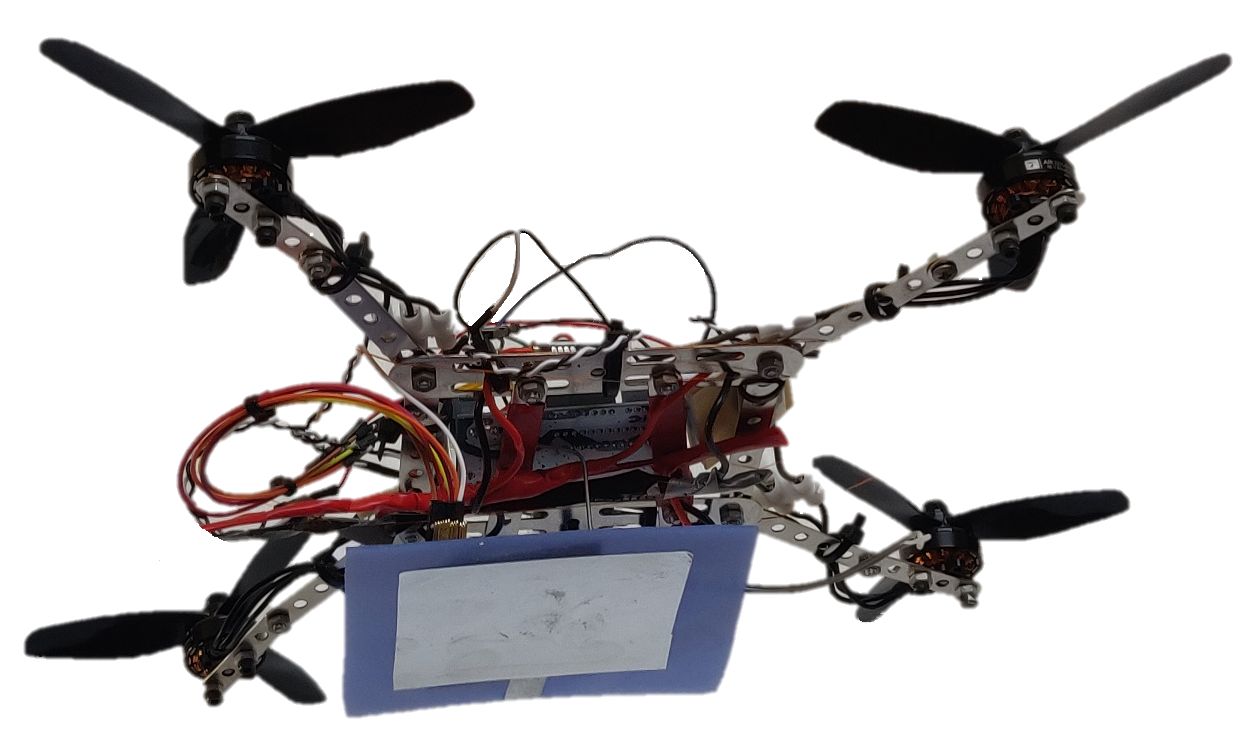
\includegraphics[width=0.5\linewidth]{drone.png}
  \caption{Afbeelding van een microstrip patch antenne bevestigd aan de onderkant van een drone. }
  \label{fig:exampleDrone}
\end{figure}

\section{Methodologie}
\subsection{Elektromagnetische Straling}
\subsubsection{Totale Electromagnetische Straling}
De totale \gls{SAR} voor het volledige lichaam ($SAT^{wb,totaal}_{10g}$) van een individu 
kan berekend worden als een eenvoudige som van de \gls{SAR}-waarden van de individuele bronnen. 
Dit is gebaseerd op de formule uit \cite{J17_kuehn2019modelling} dewelke aanneemt dat het mobiele apparaat 
tegen het oor van zijn gebruiker gehouden wordt. Hierdoor worden alle waarden in locale \gls{SAR}-waarden voor het hoofd uitgedrukt.
In dit netwerk is de plaats van het mobiele apparaat echter  niet  gekend wat zou leiden tot incorrecte conclusies. Bijgevolg 
zal alles uitgedrukt worden in functie van het volledige lichaam.

\begin{equation} 
\begin{aligned}
SAT^{wb,totaal}_{10g} = SAT^{wb,myUE}_{10g} +  SAT^{wb,myUABS}_{10g} \\
+ SAT^{wb,otherUE}_{10g} + SAT^{wb,otherUABSs}_{10g}
\end{aligned}
\label{eq:overallSARwb}
\end{equation}

In bovenstaande formule staat $wb$ voor whole body oftewel het volledige lichaam en $UE$ voor User Equipment oftewel het mobiele apparaat op de grond.
De eerste parameter, $SAT^{wb,myUE}_{10g}$, duidt de geabsorbeerde elektromagnetische straling aan komende van de gebruik zijn eigen apparaat.
Ondanks het feit dat de \gls{UL} straling bedoeld is voor de \gls{UABS} die deze gebruiker behandeld,
een deel van deze straling wordt ook geabsorbeerd door de gebruiker zelf. 
Dit komt vanwege het omnidirectionele karakter van de mobiele apparaat zijn antenne.
Een tweede parameter is $SAT^{wb,myUABS}_{10g}$ dewelke de straling aanduid veroorzaakt door \gls{DL} dataverkeer, komende van de \gls{UABS} die deze gebruiker behandeld.
Als derde parameter hebben we $SAT^{wb,otherUE}_{10g}$ dewelke de straling aanduidt veroorzaakt door andere gebruikers hun mobiel apparaat.
Als laatste stelt $SAT^{wb,otherUABSs}_{10g}$ de \gls{DL} straling voor komende van alle \gls{UABS}en die andere gebruikers behandelen.
Een illustratie is te vinden in figuur \ref{fig:networkIllustration} waarbij de groene pijl straling in het nabije veld voorstelt en alle andere 
pijlen straling in het verre veld voorstellen.

\begin{figure}[h!]
\centering
  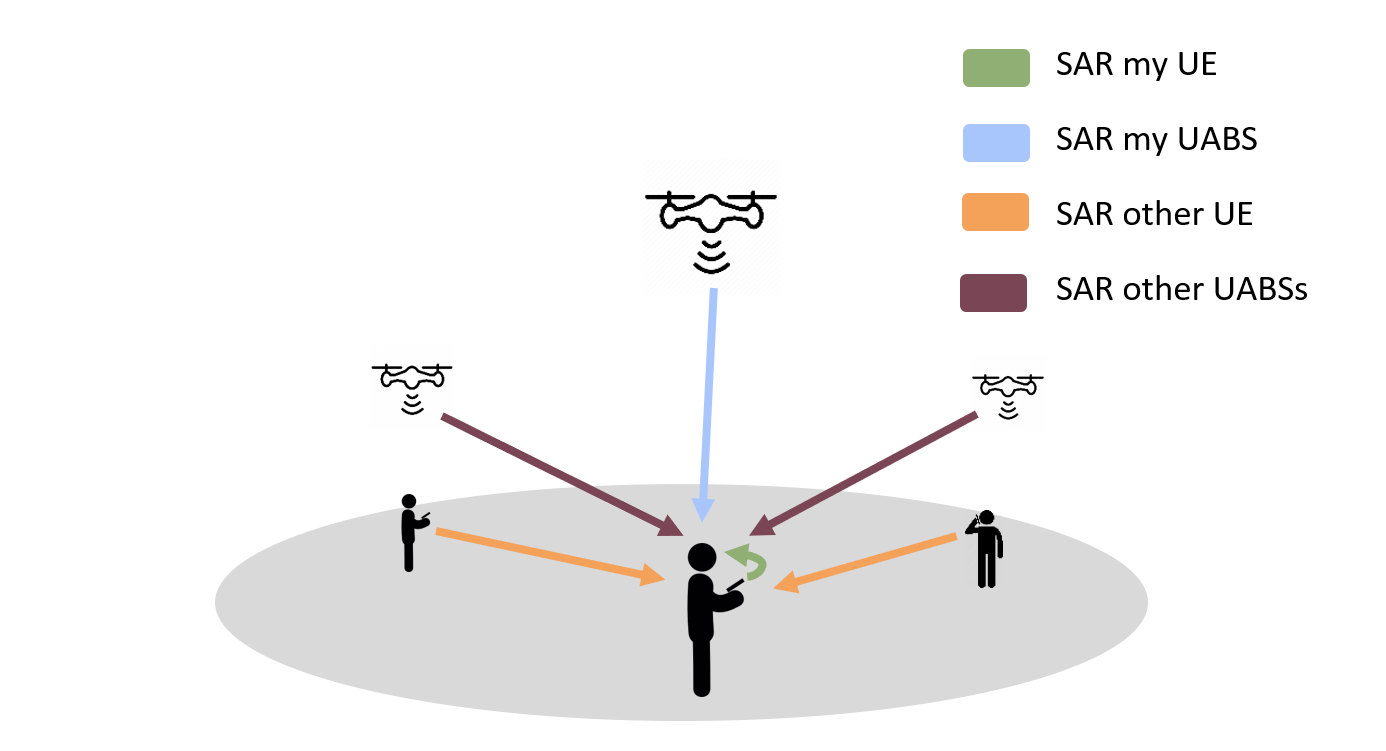
\includegraphics[width=\linewidth]{networkIllustrationSARSources.png}
  \caption{Deze illustratie toont hoe de gemiddelde gebruiker (hier getoond in het midden) be\"invloed worden door verschillende bronnen van elektromagnetische straling.}
  \label{fig:networkIllustration}
\end{figure}

\subsubsection{Electromagnetische straling van een indivuele bron}
\label{sec:calculatingexposure}

Om de totale elektromagnetische straling te vinden waaraan de gebruiker is blootgesteld, dient eerst
de straling van elke individuele bron berekend te worden.
Dit wordt gedaan met formule  \ref{eq:singleexposure} en is van toepassing voor alle bronnen in het verre veld.
Dit houdt in: alle  \gls{UABS}'s en alle mobiele apparaten die niet tot de gebruiker behoren.
De elektromagnetische veldsterkte $E$ voor het individu $u$ komende van een brom $i$ wordt als volgt berekend.

\begin{equation}
E_i(u) [V/m] = 10^{\frac{ES(u)[dBm] - 43.15 + 20*\log(f [MHz])- PL(u) [dB]}{20}}
\label{eq:singleexposure}
\end{equation}

Het berekenen van de effectieve straling (ES) voor een gebruiker $u$ vereist eerst om de  \gls{EIRP} te hebben berekend 
 \cite{J6_originalExposureFormula,J1}. Dit kan bekomen worden door de zendvermogen $P_t$ op te tellen met de zendversterking $G_t$
 en het kabelverlies $L_t$ ervan af te trekken.
 Deze formule dient echter uitgebreid te worden zodoende dat er rekening gehouden wordt met signaalverzwakking die komt met
 verschillende stralingspatronen. Deze waarde hangt af van de hoek tussen de gebruiken en de richting waarnaar de antenne wijst. 
 De signaalverzwakking bij een \gls{isotropicradiator} is altijd nul ongeacht de hoek.
 Dit leidt tot de volgende formule.

\begin{equation}
\begin{aligned}
RRP [dBm] = P_t [dBm] + G_t [dBi]- L_t [dB]\\
     - attenuation(u) [dB]
\end{aligned}
\label{eq:eirp}
\end{equation}

De gebruikte frequentie $f$ in formule \ref{eq:singleexposure} is uitgedrukt in MHz. Aangezien 
\gls{LTE} gebruikt wordt zal deze waarde 2600 MHz bevatten.

Als laatste dient formule \ref{eq:singleexposure} ook het padverlies $PL$ te kennen.
Een geschikt propagatie model dient gekozen te worden. Hier wordt geopteerd voor het 
Walfish-Ikegami model aangezien deze goed presteerd voor femtocell netwerken in stedelijke gebieden \cite{J2}.

\subsubsection{Samenvoegen van meerdere bronnen}

De totale elektromagnetische straling $E_{tot}$ in een bepaald punt, komende van alle verschillende bronnen kan berekend worden 
m.b.v. formule \ref{eq:totalexposure}. Hierin staat $E_i$ voor de elektromagnetische veldsterkte voor dat punt komende van bron $i$
en $n$ staat voor alle bronnen in het verre veld van een bepaalde categorie wat hier ofwel \gls{UABS}'s of mobiele apparaten van andere personen zijn.
$E_{tot}$ zal berekend worden in elk punt waar er zich een gebruiker bevindt.
\begin{equation}
E_{tot} [V/m] = \sqrt{\sum_{i=1}^{n} (E_i [V/m]) ^2}
\label{eq:totalexposure}
\end{equation}

\subsubsection{Omzetten van elektromagnetische veldsterkrte naar \gls{SAR}}

Formule \ref{eq:overallSARwb}  verwacht dat de \gls{SAR} waarden in functie van het volledige lichaam uitgedrukt zijn.
Om de elektromagnetische veldsterkte te kunnen omzetten daar deze \gls{SAR}-waarden dient er een onderscheid gemaakt te worden 
tussen bronnen in het nabije veld ($SAR^{wb,nf}$) en het verre veld ($SAR^{wb,ff}$).
$SAR^{wb,myUE}_{10g}$ is een bron waarbij de gebruiker zich in het nabije veld bevindt terwijl 
de gebruiker zich voor alle andere bronnen in het verre veld bevindt.

Het omzetten van deze waarden gebeurd door middel van een conversie constante dewelke gebaseerd is op 
Duke van de Virtual Family. Duke is een 34 jarige man met een gewicht van 72 kg, een hoogte van 1.74 en 
een BMI van 23.1 kg/m \cite{J22_plets2015joint}. 
Onderzoek toont aan dat de conversie constante voor WiFi in het verre veld $0.0028 \frac{W/kg}{W/m^2}$ bedraagt
en  0.0070 $\frac{W/kg}{W}$ in het nabije veld \cite{J22_plets2015joint}.
WiFi maakt gebruik van het 2400 MHz spectrum wat heel dichtbij \gls{LTE} valt (2600 MHz). Daarom 
wordt in \cite{J22_plets2015joint} aangenomen dat de conversie  constante ook van toepassing is voor \gls{LTE}.
Het berekenen van \gls{SAR} in het verre veld  wordt als volgt gedaan:

\begin{equation}
S [W/m^2]= \frac{(E_{tot} [V/m])^2}{337}
\label{eq:flux}
\end{equation}
\begin{equation}
SAR^{wb,ff}_{10g} [W/kg]= S [W/m^2]* 0.0028 \left[\frac{W/kg}{W/m^2}\right]
\label{eq:DLconversion}
\end{equation}

De constante is vergelijking \ref{eq:DLconversion} zet de \gls{power flux density} $S$ om  naar de verwachtte $SAR^{ff,wb}_{10g}$.
Om dit mogelijk te maken moet 
de uitkomst van formule \ref{eq:totalexposure} eerst nog omgezet worden naar \gls{power flux density} met behulp van formule
\ref{eq:flux}.

De \gls{SAR} die veroorzaakt wordt door het mobiel apparaat in het nabije veld kan gevonden worden door 
het zendvermogen $P_{tx}$ van het  apparaat te vermenigvuldigen met de conversie constante voor het nabije veld
en is berekend als volgt:
\begin{equation} 
SAR^{wb,nf}_{10g} \left[\frac{W}{kg}\right] = 0.0070 \left[\frac{W/kg}{W}\right] * P_{tx} [W]
\label{eq:ulToSar}
\end{equation}

De energie die door het mobiele aparaat wordt gebruikt kan berekend worden met formule \ref{eq:powerUE} \cite{J22_plets2015joint}.
\begin{multline} 
P_{tx}^{UE} = min \big\{P_{max} [dBm] , \\
 P_{pusch} [dBm] + \alpha * PL [dB] + 10log(M) + \sigma \big\}
\label{eq:powerUE}
\end{multline}


Hierbij staat $P_{max}$ voor het maximale toegestane zendvermogen van het mobiele apparaat wat voor LTE 23 dBm bedraagd.
Dit is echter in het slechste geval. De effectieve waarde ligt dankzij power control doorgaans lager.
$P_{pusch}$ is de minimale energie vereist door de 
\gls{UABS} en bedraagt hier -120 dBm. 
$\alpha$ is de compensatiefactor voor het padverlies en is gelijk aan \'e\'en wat hier volledige compensatie betekend \cite{J32,J33}.
Voor het 20 MHz kanaal in deze paper zal $M$ gelijk zijn aan 100 en
 zal $\sigma$,  als correctiefactor, nul bedragen \cite{J22_plets2015joint,J32}.

\subsection{Microstrip Patch Antenne}
Een microstrip patch antenne is gekozen vanwege zijn eenvoudige productieproces maar voornamelijk vanwege het
 lage gewicht en aerodynamica wat heel voordelig is wanneer het aan een drone gekoppeld wordt \cite{J13_microstripadvantages}.

De dimensies van de antenne hangen af van de gebruikte frequentie en de eigenschappen van het di\"electrisch substraat.
De antenne zal opereren met een frequentie $f_0$ van 2.6 GHz. 
Elk substraat heeft een di\"electrische constante $\epsilon_r$ dat de doorlaatbaarheid 
van het substraat aanduid en hangt af van het gebruikte materiaal.
Substraten met een hoge di\"electrische constante en kleine hoogte zullen de dimensies van de antenne reduceren 
terwijl  een lager di\"electrische constante met een hogere hoogte de performantie van de 
antenne zullen bevorderen \cite{J14_antennadesign,J15_antennadesign}. 
Voor dit onderzoek is glas gekozen vanwege zijn hogere di\"electrische constante
 $\epsilon_r = 4.4$ ten opzichte van andere materialen zoals Teflon met een di\"electrische constante
van $\epsilon_r = 2.2$ \cite{J14_antennadesign}. 
Glass met een hoogte van 2.87 mm 
zal de dimensies van het volledige antenne opperlakte verminderen wat 
voordelig is bij de beperkte ruimte die beschikbaar is op een drone.

\begin{table}[h!]
\centering
\begin{tabular}{|l|c|l|}
\hline
 Beschrijving            & Symbool          & Waarde         \\    \hline
 Middenfrequentie      & $f_0$           & 2600 MHz       \\ 
 Di\"electrische constante    & $\epsilon_r$    & 4.4         \\ 
 Hoogte van het substraat & $h$             & 0.00287 m    \\ \hline
\end{tabular}
\caption{Overzicht van de configuratie parameters}
\label{table:antennaparas}
\end{table}

De dimensies van de stralingsplaat kunnen berekend worden met de formules uit \cite{J14_antennadesign,J15_antennadesign}.
Dit leidt tot een stralingsplaat van 35.09 mm bij 26.55 mm en  een grondplaat van minstens 52.40 mm bij 43.80 mm.
De resulterende microstrip patch antenne is ge\"illustreerd in figuur \ref{fig:basicpatchantenna} en zal resulteren 
in het stralingspatroon getekend in figuur \ref{fig:radpattern}.
\begin{figure}[h!]
\centering
  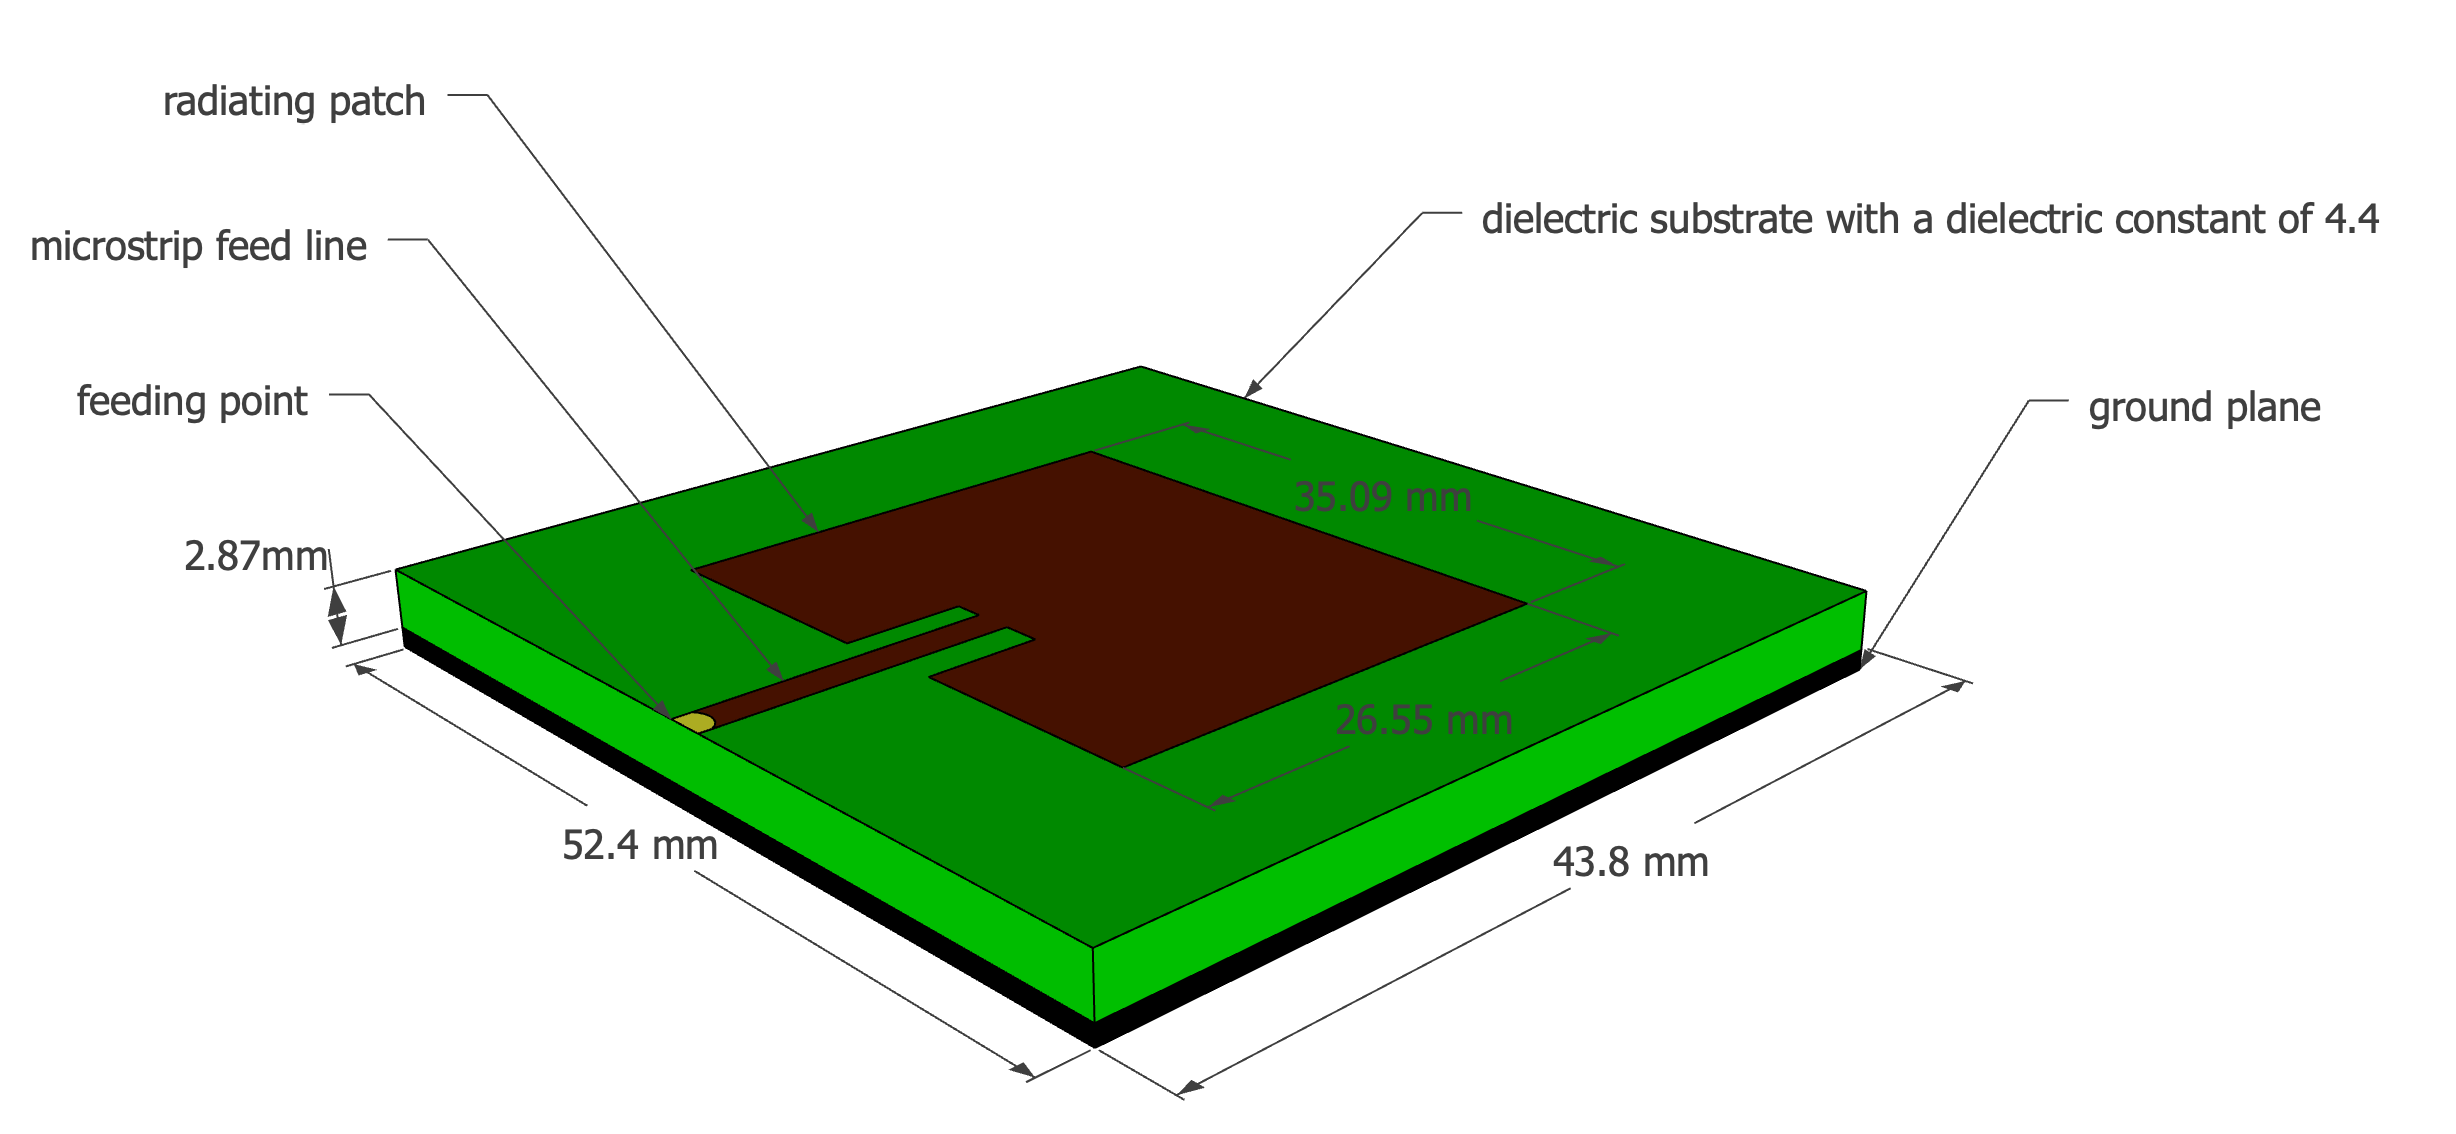
\includegraphics[width=\linewidth]{MicrostripAntenna.png}
  \caption{Schema van een microstrip patch antenne.}
  \label{fig:basicpatchantenna}
\end{figure}


\begin{figure}[!htb]
\minipage{0.50\linewidth}
  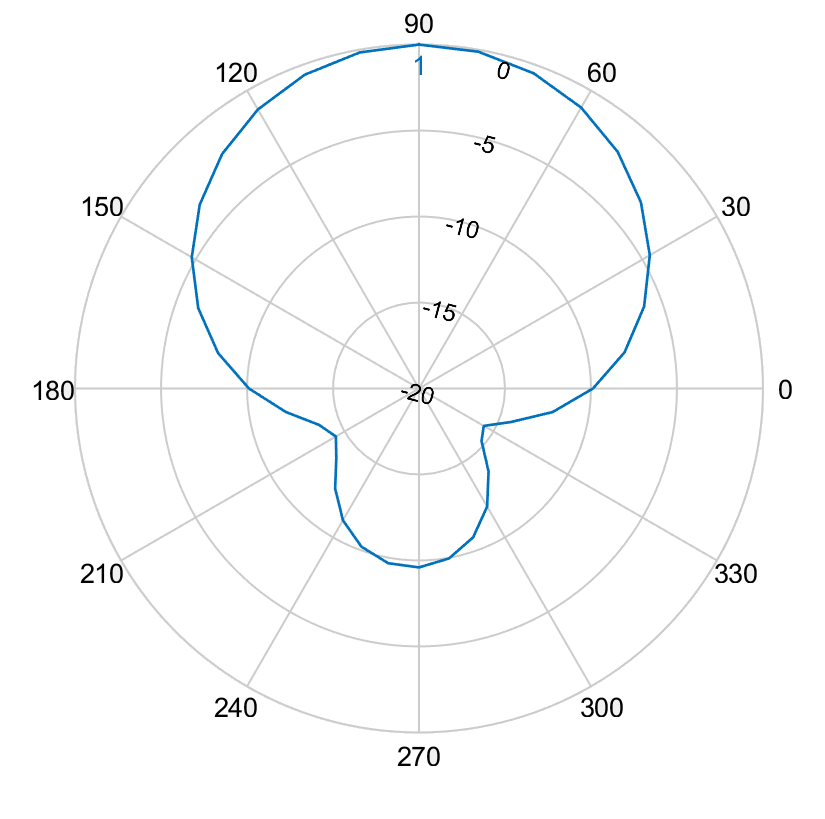
\includegraphics[width=\linewidth]{pattern2/ep.png} 
\endminipage\hfill
\minipage{0.50\linewidth}%
  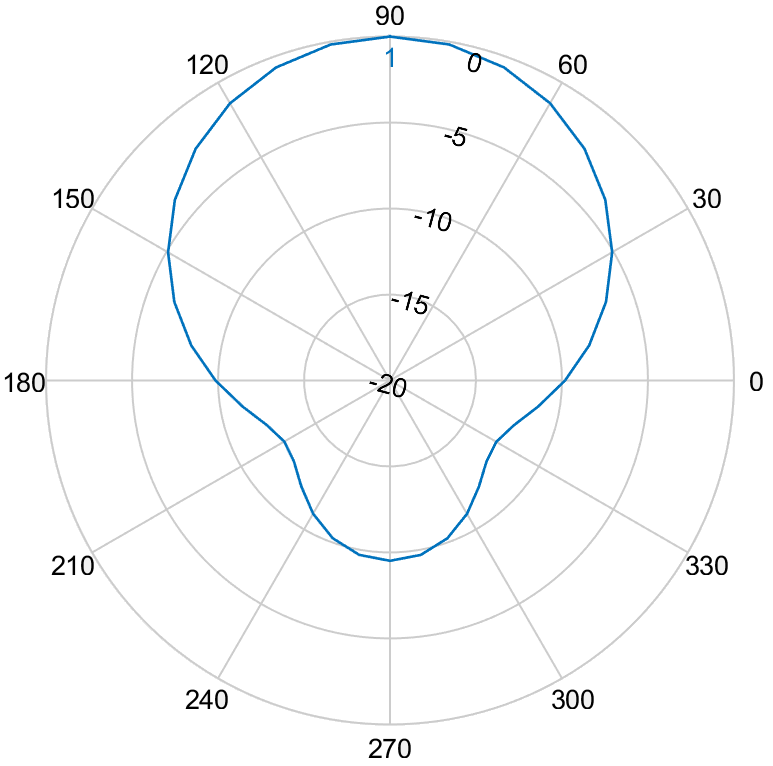
\includegraphics[width=\linewidth]{pattern2/hp.png}
\endminipage
  \caption{Links is het stralingspatroon voor het E-vlak en rechts voor het H-vlak.}
\label{fig:radpattern}
\end{figure}

\subsection{Optimaliseren van het netwerk}

Deruyck et al. bespreekt in \cite{J1} hoe een traditioneel mobiel netwerk geoptimaliseerd kan worden naar elektromagnetische straling of energieconsumptie.
Hoewel een toenemend zendvermogen wel degelijk resulteert in hogere elektromagnetische veldsterkte is deze regel niet van 
toepassing indien we het energieverbruik bekijken over het hele netwerk heen. 
De auteurs van \cite{J1} tonen een omgekeerd equivalente relatie aan.
De reden hierachter is dat het vaak minder energie kost om de elektromagnetische straling van een reeds actieve base station 
verder te laten toenemen i.p.v.  een nieuwe base station te activeren. Dit leidt tot de volgende fitness functie dewelke
gebaseerd is op \cite{J1}.

\begin{equation} 
f = w * \left(1 - \frac{E_m}{E_{max}}\right) + (1 - w)*\left(1 - \frac{P}{P_{max}}\right) * 100
\label{eq:fitnessfunction}
\end{equation}

Formule \ref{eq:fitnessfunction} geeft een gewicht terug dat aanduid hoe goed het netwerk preseteerd.
$w$ is de belangrijkheidsfactor die loopt van 0 tot 1, grenzen inbegrepen. Een $w$ gelijk aan 0 betekend
dat elektromagnetische straling niet belangrijk is. Een dergelijk network wordt een \gls{PwrC Opt} netwerk genoemd.
Aan de andere kant, een $w$ gelijk aan 1 impliceert dat het minimaliseren van elektromagnetische bloodstelling top prioriteit is
en zal bijgevolg resulteren in een \gls{Exp Opt} netwerk. $P_{max}$ is het energieverbruik van alle \gls{UABS}'s op maximaal 
zendvermogen, ongeacht of ze 
op non-actief staan of niet.
$P$ representeerd de effectieve verbruikte energie van het huidig ontwikkelde netwerk.
$E_m$ is de elektromagnetische straling van de gewogen gemiddelde gebruiken van het huidig ontwikkelde netwerk en 
$E_{max}$ is dezelfde waarde maar met alle \gls{UABS}'s op maximaal zendvermogen.

Bij het optimaliseren van het netwerk is het niet enkel belangrijk om  de gemiddelde gebruiker te overwegen maar ook het limiteren 
van extrema \cite{J1}. 
Daarom wordt er gebruik gemaakt van het gewogen gemiddelde waarbij niet enkel rekening gehouden wordt met de mediaan maar ook 
met het 95\textsuperscript{ste} percentiel. Dit leidt tot formule \ref{eq:em} waarbij 
  $w_1$ en  $w_2$ de gewichten zijn van respectievelijk de mediaan en het 95\textsuperscript{ste} percentiel.
 Aangezien verondersteld wordt dat beiden waarden een gelijkwaardige rol spelen zullen beiden een gewicht van 0.5 krijgen. 

\begin{equation} 
E_m = \frac{w_1 * E_{50} + w_2 * E_{95}}{w_1 + w_2}
\label{eq:em}
\end{equation}

\begin{figure}[h!]
  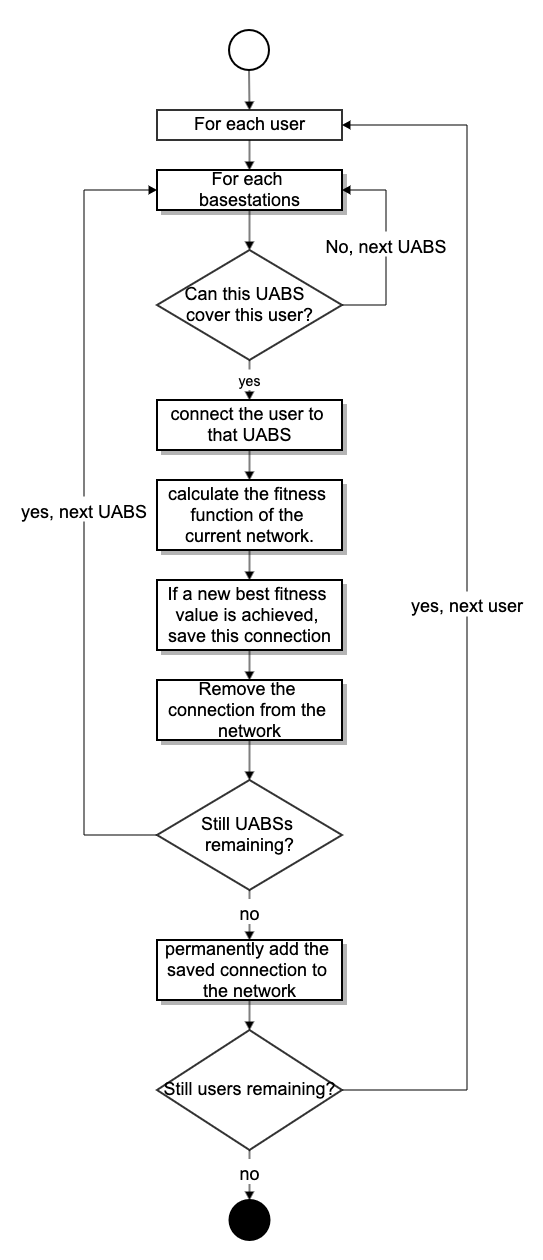
\includegraphics[height=0.8\textheight]{decisionAlgoFlowChart.png}
  \caption{Flowchart of the decision algorithm.}
  \label{fig:decisionAlgoFlowChart}
\end{figure}

\subsection{Simulatie Tool}

\subsubsection{Hoofdalgoritme}
In eerste instantie dient een beschrijving van het gebied voorzien te worden. Dit wordt verwezenlijkt met behulp van 
zogenaamde shape-bestanden. Deze bestanden bevatten een volledige beschrijving van de vorm van elk gebouw. Vervolgens 
worden gebruikers uniform verdeeld over het gebied en zal er een tijdelijke \gls{UABS} geplaatst worden boven elke gebruiker.
Nu is het aan het beslissingsalgoritme om te bepalen welke \gls{UABS}'s effectief zullen blijven en hoe hoog het zendvermogen van elke \gls{UABS}
zal zijn. Eens het beslissingsalgoritme voltooid is zal de tool controleren of het nummer van online drones niet meer is dat 
de capaciteit van de stockageruimte toelaat. Indien dit wel het geval is zullen drones offline gehaald worden, beginnend bij 
drones die het minste personen behandelen.

\subsubsection{Beslissingsalgoritme}

Het oplossen van het netwerk is de verantwoordelijkheid van het beslissingsalgoritme en start met het berekenen van het padverlies tussen 
alle gebruikers en tussen gebruikers en drones. Hierna doorloopt het algoritme elke gebruiker waarbij getracht wordt deze te verbinden 
met elke mogelijke \gls{UABS}. Deze verbinding is niet altijd mogelijk omdat een \gls{UABS} al reeds verzadigd kan zijn met andere gebruikers of 
de \gls{UABS} is zo ver verwijderd van deze gebruiker dat het de maximale toegestane zendvermogen zou overschreiden.
Indien een verbinding toch mogelijk is zal de gebruiker met deze \gls{UABS} verbonden worden en zal een score toegekend worden met behulp van 
de fitness functie uit vergelijking \ref{eq:fitnessfunction}. 
Dit proces wordt herhaald voor elke \gls{UABS}. Uitsluitend de verbinding dat resulteert in de beste score voor het volledige netwerk 
zal gebruikt worden. 
Op deze mannier zal elke gebruiker de beste oplossing krijgen vanuit de huidige toestand van het netwerk.
In andere woorden, elke gebruiker wordt geoptimaliseerd en niet het netwerk zelf. Er wordt echter wel aangenomen dat 
op deze manier het gemiddelde netwerk zelf ook optimaal zal zijn.
Wanneer de laatste gebruiker behandeld is geweest, bekomen we een volledig netwerk voor een ongelimiteerd aantal drones.
Het network wordt vervolgens terug aan het hoofdalgoritme gegeven voor eventuele verdere afhandeling.
Een stroomdiagram van dit algoritme is gegeven in figuur \ref{fig:decisionAlgoFlowChart}.

%%%%%%%%%%%%%%%%%%%%%%%%%%%%%%%%%%%%%%%%%%%%%%%%%%%%%%%%%%%%%%%%%%%%%%%%%%%%%%%%%%%%%%%%%%%%%%%%%%%%%%%%%%%%%%%%%%%

\section{Scenario's}

De standaard configuratie is gegeven in tabel \ref{table:defaultconf} en is altijd van toepassing tenzij anders vermeld.
\begin{table}[!htb]
\centering
\begin{tabular}[t]{ll}
        \toprule
        \multicolumn{2}{l}{\textbf{Mobiel netwerk}} \\
        \hline
        \hspace{3mm}  technologie        & LTE     \\
        \hspace{3mm}  frequentie         & 2.6 GHz \\
        \hspace{3mm}  Power offset ($P_{pusch}$)            & -120 dBm  \\
        \hspace{3mm}  Compenstatie voor padverlies ($\alpha$)   & 1  \\
        \hspace{3mm}  Correctie waarde                    & 0 dBm  \\
        \hspace{3mm}  Aantal resource blokken      & 100  \\
        \hline
        \multicolumn{2}{l}{\textbf{Drone}} \\
        \hline  
        \hspace{3mm}  energie drone        & 13.0 A   \\
        \hspace{3mm}  gemiddelde snelheid        & 12.0 m/s \\
        \hspace{3mm}  gemiddeld energieverbruik      & 17.33 Ah    \\
        \hspace{3mm}  voltage batterij       & 22.2 V \\
        \hline
        \multicolumn{2}{l}{\textbf{Femtocell antenna}} \\
        \hline  
        \hspace{3mm}  maximum $P_{tx}$          & 33 dBm   \\
        \hspace{3mm}  richting van de antenne   & neerwaards   \\ 
        \hspace{3mm}  zendversterking           & 4 dBm   \\ 
        \hspace{3mm}  kabelverlies               & 2 dBm   \\ 
        \hspace{3mm}  implementation loss       & 0 dBm   \\
        \hspace{3mm}  stralingspatroon         & EIRP or\\
         \hspace{3mm}                           & microstrip patch\\
        \hspace{3mm}  vlieghoogte                & 100m  \\
        \hline
        \multicolumn{2}{l}{\textbf{UE Antenna}} \\
        \hline 
        \hspace{3mm} hoogte                     & 1.5m vanaf de vloer      \\ 
        \hspace{3mm} zendversterking                      & 0 dBm   \\ 
        \hspace{3mm} kabelverlies              & 0 dBm   \\ 
        \hspace{3mm} stralingspatroon         & EIRP  \\
        \hspace{3mm} aantal aanwezig in het netwerk         & 224  \\
        \toprule
\end{tabular}
\caption{Overzicht van de waarden voor een standaard configuratie.}
\label{table:defaultconf}
\end{table}

Drie scenario's zullen onderzocht worden. Het eerste zal \'e\'en enkele gebruiker en 
 \'e\'en enkele drone overwegen 
voor het gehele netwerk. De \gls{SAR}, elektromagnetische straling, energieverbruik  en 
het nodige zendvermogen van de antenne zullen onderzocht worden voor verschillende vlieghoogtes.

Bij het tweede scenario zal het netwerk uitgebreid worden met meerdere gebruikers maar 
er zal nog steeds uitsluitend  \'e\'en drone aanwezig zijn. De eerste onderzochte parameter 
is een varierende vlieghoogte gaande van 20 meter tot 200 meter. Hierbij zullen 224 gebruikers 
uniform verdeerld worden over het centrum van Gent. Dit is de gemiddelde populatiegroote op 
een werkdag om 17 uur in Gent \cite{J2}.
De tweede parameter is een varierende population lopend van 50 tot 600 gebruikers. Hierbij 
zal de vlieghooghte vastgezet worden op 100 meter \cite{J2}.
Het energieverbruik, electromagnetische straling en \gls{SAR} zullen onderzocht worden 
onderzochte parameter.

Een derde scenario is sterk gelijkend aan het vorige. Dezelfde twee parameters zullen onderzocht 
worden maar nu voor een onbeperkt aantal \gls{UABS}'s.

Vier configuraties zijn mogelijk voor elke onderzochte parameter in elk scenario.
Er zijn namelijk twee antennes, een \gls{isotropicradiator} en een microstrip patch antenne die
beide kunnen opereren in een \gls{PwrC Opt} netwerk en een \gls{Exp Opt} netwerk. Dit maakt een totaal van 4 configuraties.
Een overzicht is gegeven in figuur \ref{fig:fourCasesMatrix}.

Het is belangrijk om op te merken dat alle meetwaarden strikt gelimiteerd zijn tot de hiervoor vermoende bronnen en 
bijgevolg enkel dataverkeer overwegen tussen de gebruiker zijn apparaat en de \gls{UABS}. 
Andere bronnen zoals connecties naar het backhaul network zullen niet overwogen worden.

\begin{figure}[h!]
  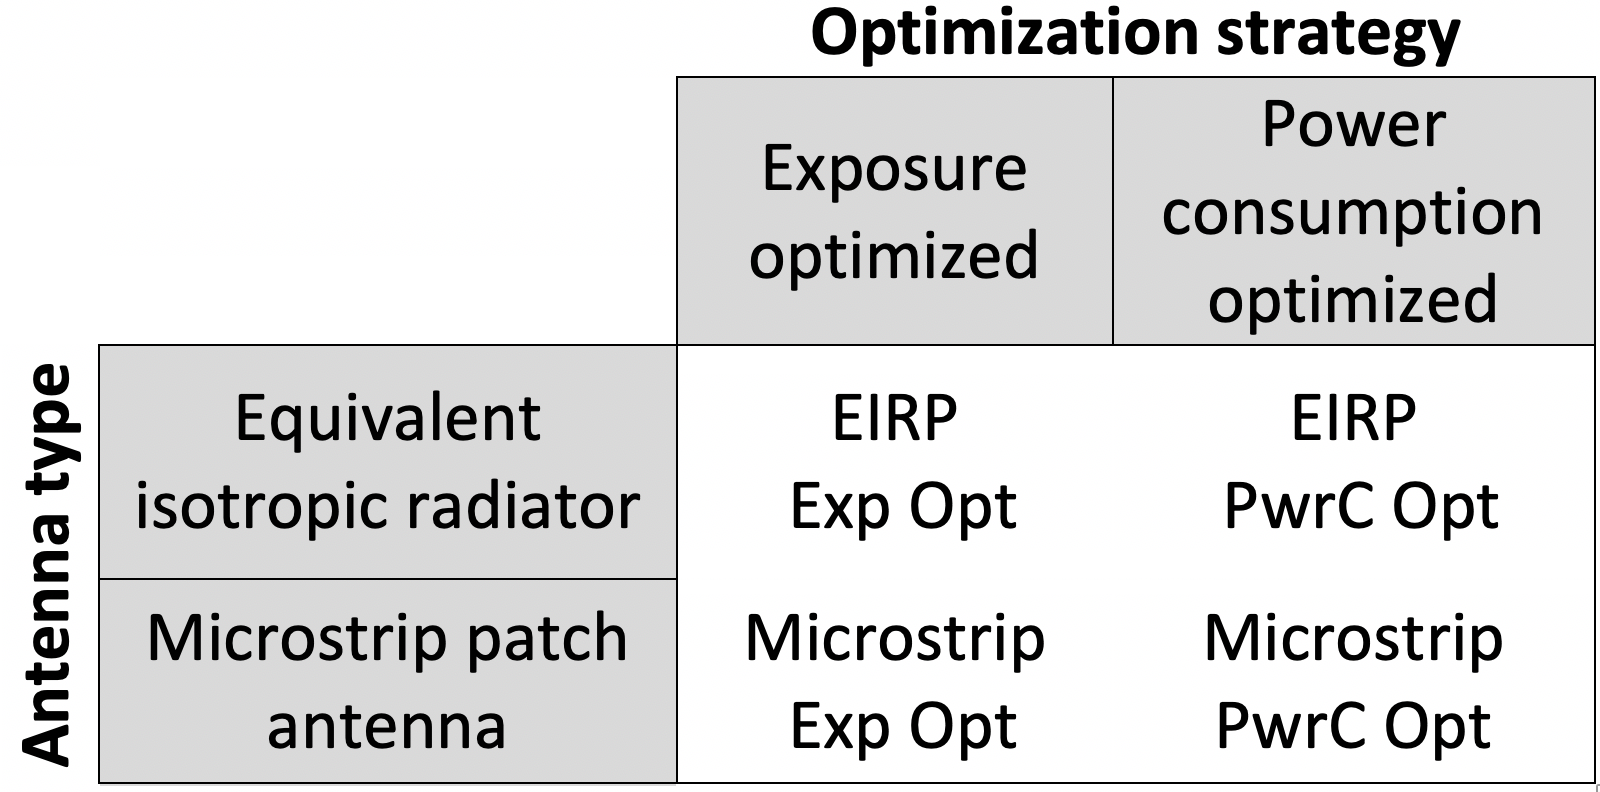
\includegraphics[width=\linewidth]{fourCasesMatrix.png}
  \caption{Matrix met de vier mogelijke configuraties.}
  \label{fig:fourCasesMatrix}
\end{figure}

\section{Results}
Vier configuraties zullen overwogen worden tijdens het evaluaren van twee parameters, zijnde 
populatie groote en vlieg hoogte. Deze parameters zullen onderzocht worden in drie scenarios 
door het gedrag van het energieverbruik, electromagnetische straling en \gls{SAR}-waarden te monitoren.
De electromagnetische straling en \gls{SAR} zullen genonmen worden van de gewogen gemiddelde gebruiker
m.b.v. vergelijking \ref{eq:em} waarbij $w_{1}$ en $w_{2}$ gelijk gesteld zijn aan 50\%. 
Elk resultaat wordt uitgemiddeld over 20 simmulaties.


\subsection{E\'en gebruik en \'e\'en \gls{UABS}}
De resultaten tonen dat voor een variabele vlieghoogte, een logaritmische relatie bestaat tussen de 
 $P_{tx}$ en de vlieghooghte.
 Dit komt door de logaritmische schaal waarin de decibels van de $P_{tx}$ zijn in uitgedrukt.
Elke keer rdat de vlieghoogte te hoog wordt neemt de $P_{tx}$ met \'e\'en dBm toe.
Voor een stanaard configurartie met een maximum $P_{tx}$ van 33 dBm en een \gls{LOS} verbinding kan een 
\gls{UABS} tot 387 m hooghte vliegen voor het verliezen van de connectie.

Dit scenario is onderzocht voor een microstrip patch antenne die energieverbruik minimaliseerd.
De gekozen optimalisatie maakt echter niet uit aangezien er uitsluitend \'e\'en \gls{UABS} beschikbaar is.
Het beslissing's algoritme bepaalt welke gebruiker met welke \gls{UABS} verbonden wordt.
Aangezien er maar een \gls{UABS} beschikbaar is is zullen beide optimalisatie technieken gelijkaardig werken.
Verder zal de gebruikte antenne ook geen verschil maken. 
De gebruiker zal zich namelijk boor beide antennes in de hoofdbeam van het stralingspatroon 
bevinden waar in beide gevallen geen verzwakking van het signaal is.

Tijdens het onderzoeken van verschillende vlieghoogte's stellen de resultaten vast  dat
\gls{UL} straling exponentieel toeneemt terwijl de \gls{DL} straling constant blijft op 
10 $nW/kg$. De reden dat de \gls{DL} straling constant blijft is vanwege power control dat ervoor zorgt
dat niet meer energie gebruikt wordt dan strikt noodzakelijk. 
Daardoor kan bevestigd worden dat de elektromagnetische straling een constante fractie is van energie en afstand.
De \gls{UL} straling start laag met 1 $nW/kg$ maar steekt de \gls{DL} straling voorbij rond de 80 meter.

\begin{figure}[]
\centering
  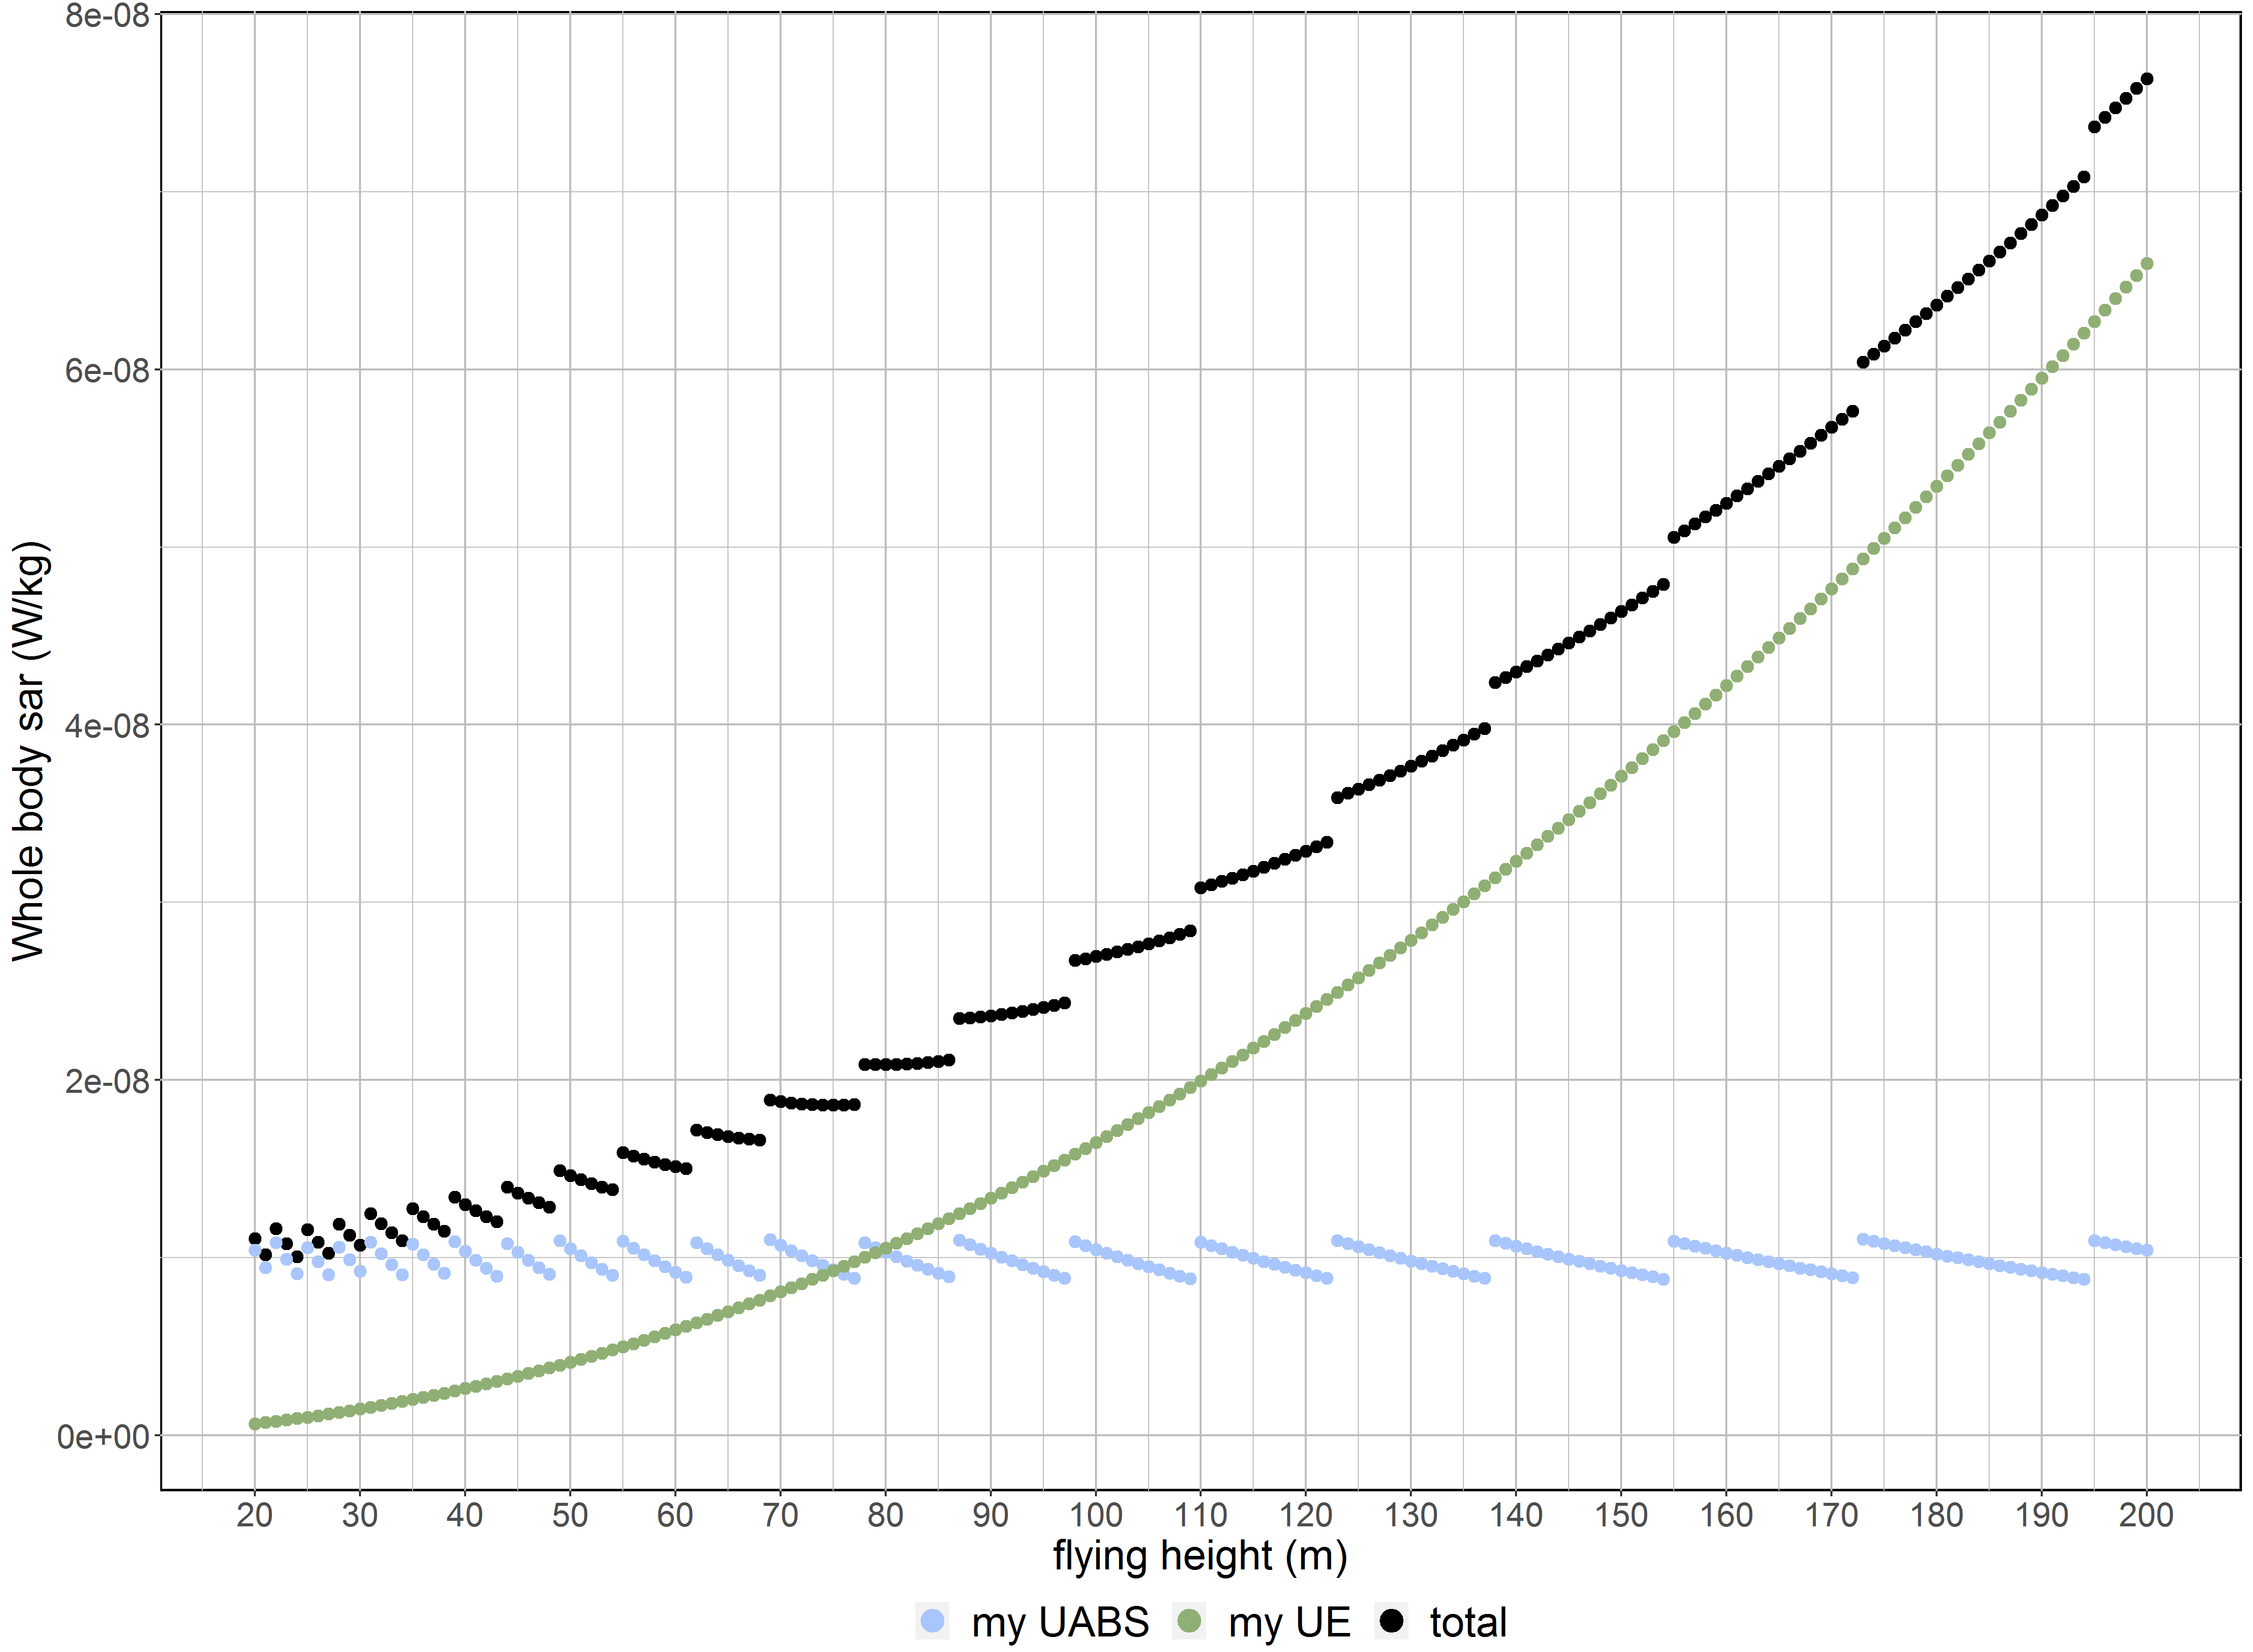
\includegraphics[width=\linewidth]{s1/fhvssar.png}
  \caption{This figure shows how SAR values from different sources are influenced by different flying altitudes.}
  \label{fig:s1_fhsar}
\end{figure}

\subsection{Toenemende populatie met \'e\'en UABS}
\subsubsection{Variabele vlieghoogte}
Een \gls{PwrC Opt} heeft een hogere elektromagnetische blootstelling in vergelijking met een
 \gls{Exp Opt} netwerk; een fenomeen dat reeds was vastgesteld bij \cite{J1}. 
Uit de resultaten van dit scenario blijkt echter dat een
\gls{PwrC Opt} niet noodzakelijk resulteert in een lager energieverbruik.
Zo zal bijvoorbeeld bij 100 m in een  \gls{EIRP} \gls{Exp Opt} netwerk
 de elektromagnetische straling van de gewogen gemiddelde gebruiker
 $1.5\ mV/m$ minder zijn maar aal het energieverbruik met $20\ mW$ toenemen.
Om dit te verstaan dient het algoritme eerst uitgelegd te worden.
Een  \gls{PwrC Opt} Netwerk zal resulteren in enkele \gls{UABS}'s met een hoog energieverbruik 
omdat het toenemen van de $P_{tx}$ van de antenne minder energie kost dan het activeren van een nieuwe \gls{UABS}.
Op dezelfde manier zal een \gls{Exp Opt} network meer \gls{UABS}'s gebruiken met een laag energie verbruik hierdoor waardoor ook de elektromagnetische straling minder zal zijn.
Wanneer een beperkt aantal \gls{UABS}'s beschikbaar zijn, zoals maar \'e\'en in dit netwerk, 
zullen enkel de \gls{UABS}'s gebruikt worden die de meeste mensen behandelen.
Daardoor is het energieverbruik en een \gls{PwrC Opt} netwerk vaak hoger.


\begin{figure}[h!]
  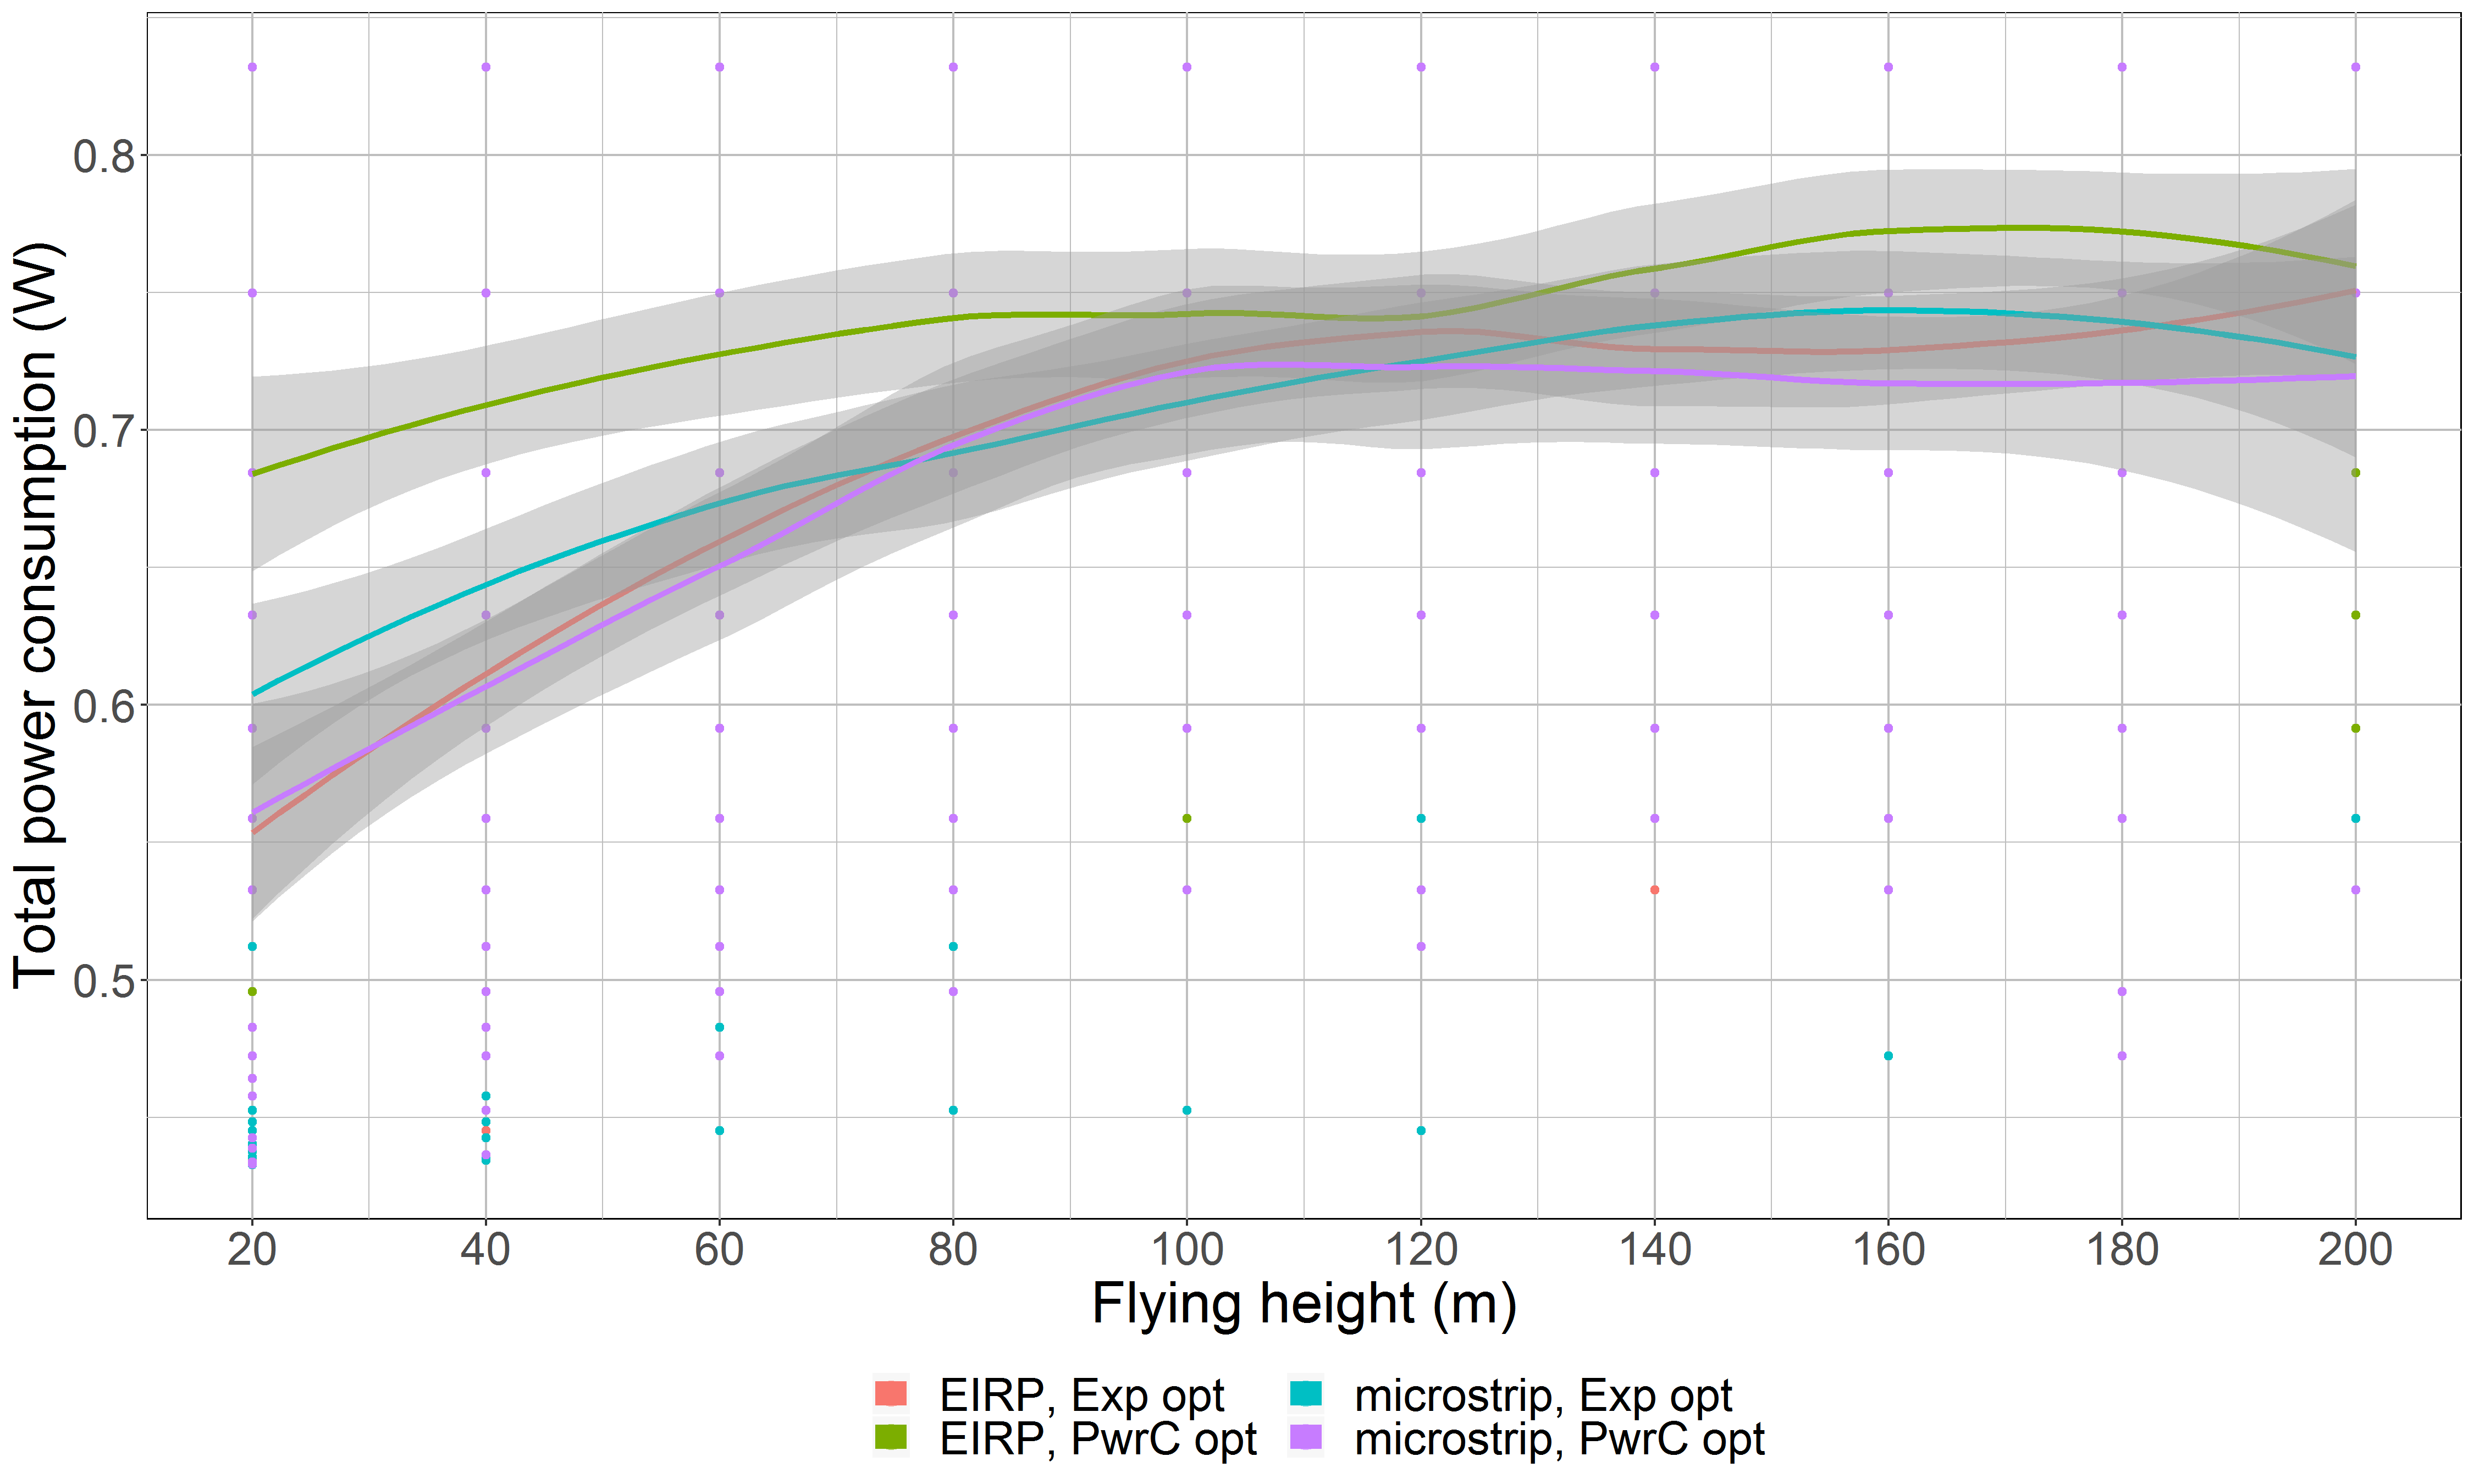
\includegraphics[width=\linewidth]{s2/fhvsdlAndPc.png}
  \caption{Fig. (a) toont hoe de vlieghooghte be\"invloedt wordt door \acs{DL} electromagnetische straking van de 
  gewogen gemiddelde gebruiker en figuur (b) toont het En energieverbruik van het volledige netwerk wanneer een enkele drone beschikbaar is.}
  \label{fig:s2a_dlAndPc}
\end{figure}

Verder stond figuur  \ref{fig:s2a_dlAndPc} Hoe de elektromagnetische blootstelling toeneemt wanneer de vlieghoogte horen wordt. 
Dit komt omdat de waarschijnlijk het op een \gls{NLOS} kleiner wordt.
Dit lijkt eveneens ook tot een hoger dekkingsgraad.
Wanneer de vlieghoogte toeneemt van 20 tot 100 m zal de dekkingsgraad met 1\% tot 2\% voor alle configuraties toenemen.
Deze toename in elektromagnetische straling's is goed dan ook niet ongelimiteerd. Een microstrip \gls{PwrC Opt}
Is op zijn hoogste punt rond 162 m en een \gls{EIRP} \gls{PwrC Opt} is op zijn hoogste punt rond 195 m.
De wederafname van elektromagnetische straling start later voor \gls{Exp Opt} netwerken 
en bevindt zich buiten de onderzochte vlieghoogte's. 
Deze wederafname is niet veroorzaakt door gebouwen maar door de grote afstand in het algemeen.

Figuur \ref{fig:s2shfourSourcesMatrix} toont de $SAR^{wb}_{10g}$ van de Gewogen gemiddelde gebruiker voor elke individuele bron.
De resultaten stellen vast dat de $SAR^{myUABS}$ dezelfde curve toont als deze van de elektromagnetische straling in figuur
figure \ref{fig:s2a_dlAndPc}.a. Dit komt omdat vergelijking \ref{eq:DLconversion} de electrische straling converteert naar \gls{SAR}
door het te multipliceren met een constante.Gedurende de gehele tijd is de $SAR^{myUABS}$
de meest dominante factor gevolgd door de straling van de gebruiker zijn eigen mobiel apparaat.
Straling komende van andere personen hun mobiel apparaat heeft amper invloed.
Als voorbeeld op een vlieghoogte van 140 m zal de gewogen gemiddelde gebruiker in een
\gls{EIRP} \gls{PwrC Opt} 2.1 $nW/kg$ Ondervinden van de  \gls{UABS} rn ron d
 0.2 $nW/kg$ van zijn eigen apparaat.
De blootstelling van andere mobiele apparaten kan verwaarloosd worden met een elektromagnetische straling van slecht
 0.03 $pW/kg$. Dit is een laag maar plausibele waarde aangezien de meeste mensen niet gedekt zijn 
en daardoor zelf geen straling veroorzaken.


\begin{figure}[h!]
  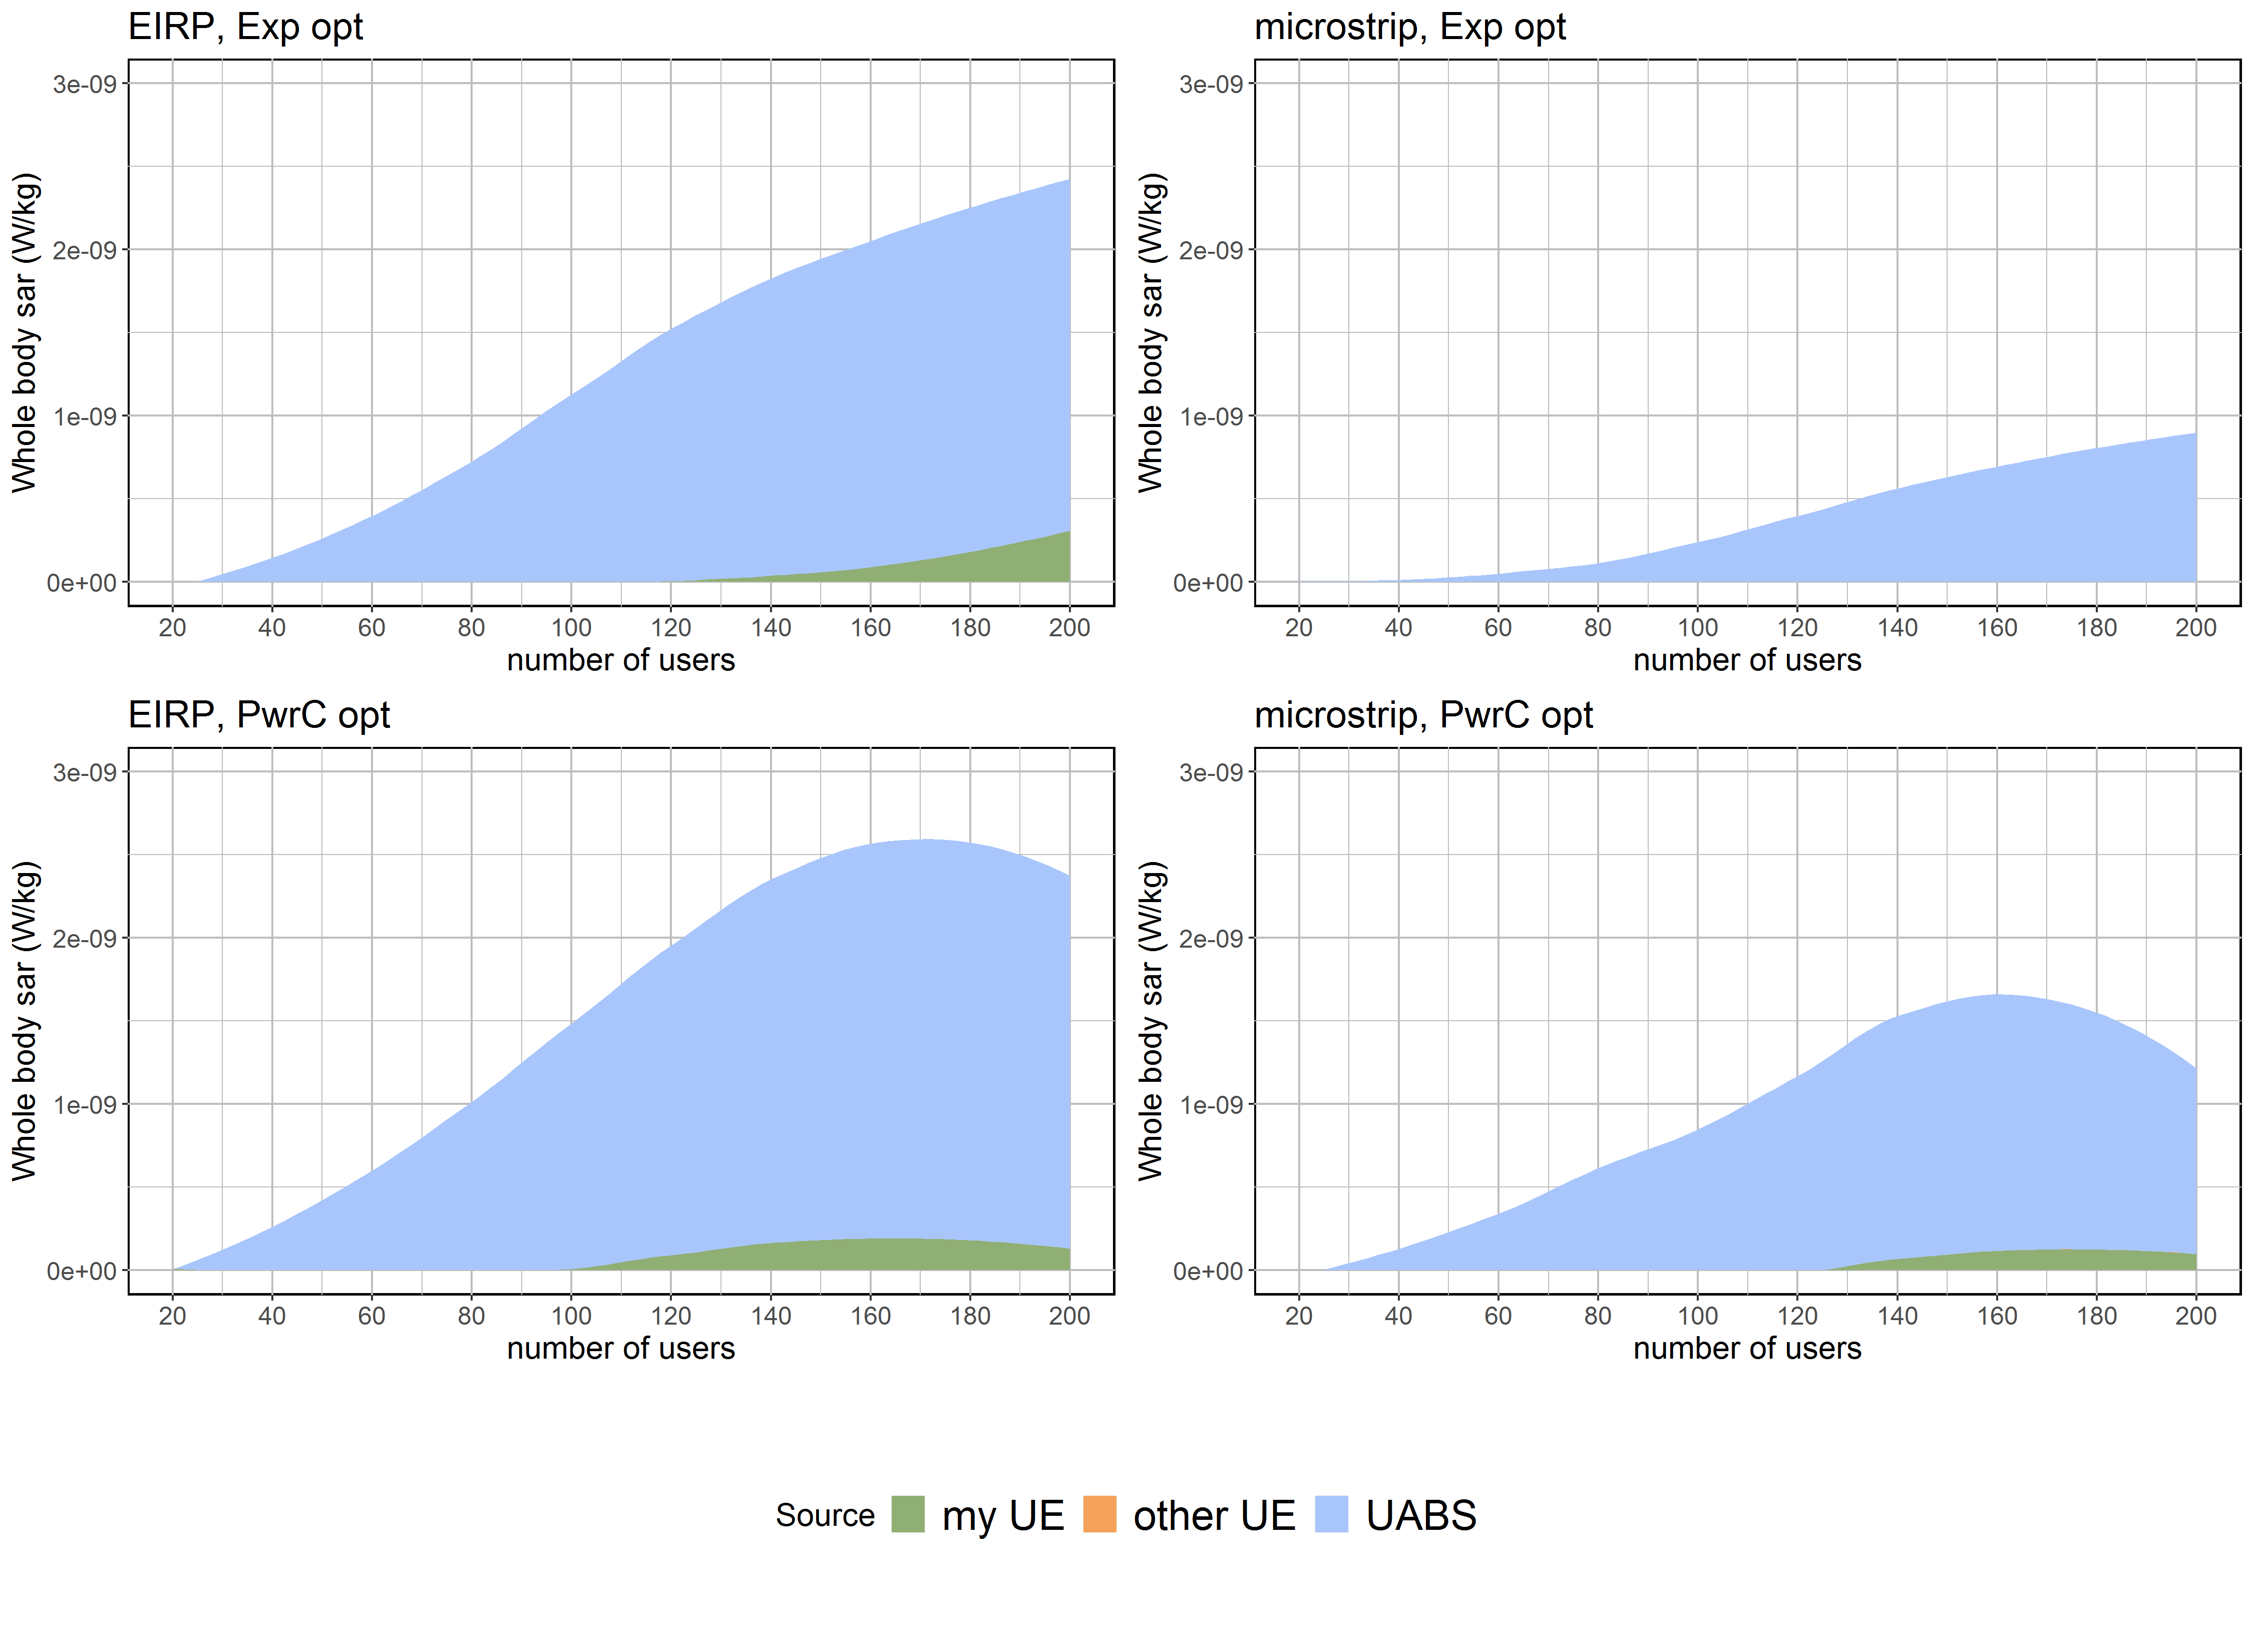
\includegraphics[width=\linewidth]{s2/fhFourSources.png}
  \caption{ Welke figuur komt overeen met een specifieke configuratie en toont hoe de 
     \acs{SAR} van verschillende bronnen be\"invloed wordt door een toenemende vlieghoogte.}
  \label{fig:s2shfourSourcesMatrix}
\end{figure}

\subsubsection{Variabele aantal gebruikers}
Het aantal gedekte gebruikers neemt lineair toe met het aantal personen aanwezig in het netwerk zoals getoond wordt op figuur
\ref{fig:s2uvsnumcovusers}.b. Het toont hoe  \gls{isotropicradiator} in staat is om meer personen te behandelen in vergelijking met eenvoudig
 microstrip patch antenna. Eveneens is een energiezuinig netwerk in staat om meer mensen te behandelen dan een netwerk die electromagnetische straling minimaliseert.
 Bijvoorbeeld met 600 gebruikers zullen 5 tot 7 extra personen behandeld kunnen worden wanneer 
 een microstrip patch antenne vervangen wordt door een  \gls{isotropicradiator}.
Door van een \gls{Exp Opt} network naar een \gls{PwrC Opt} netwerk te gaan kan er \'e\'en extra persoon 
behandeld worden.

\begin{figure}[h!]
  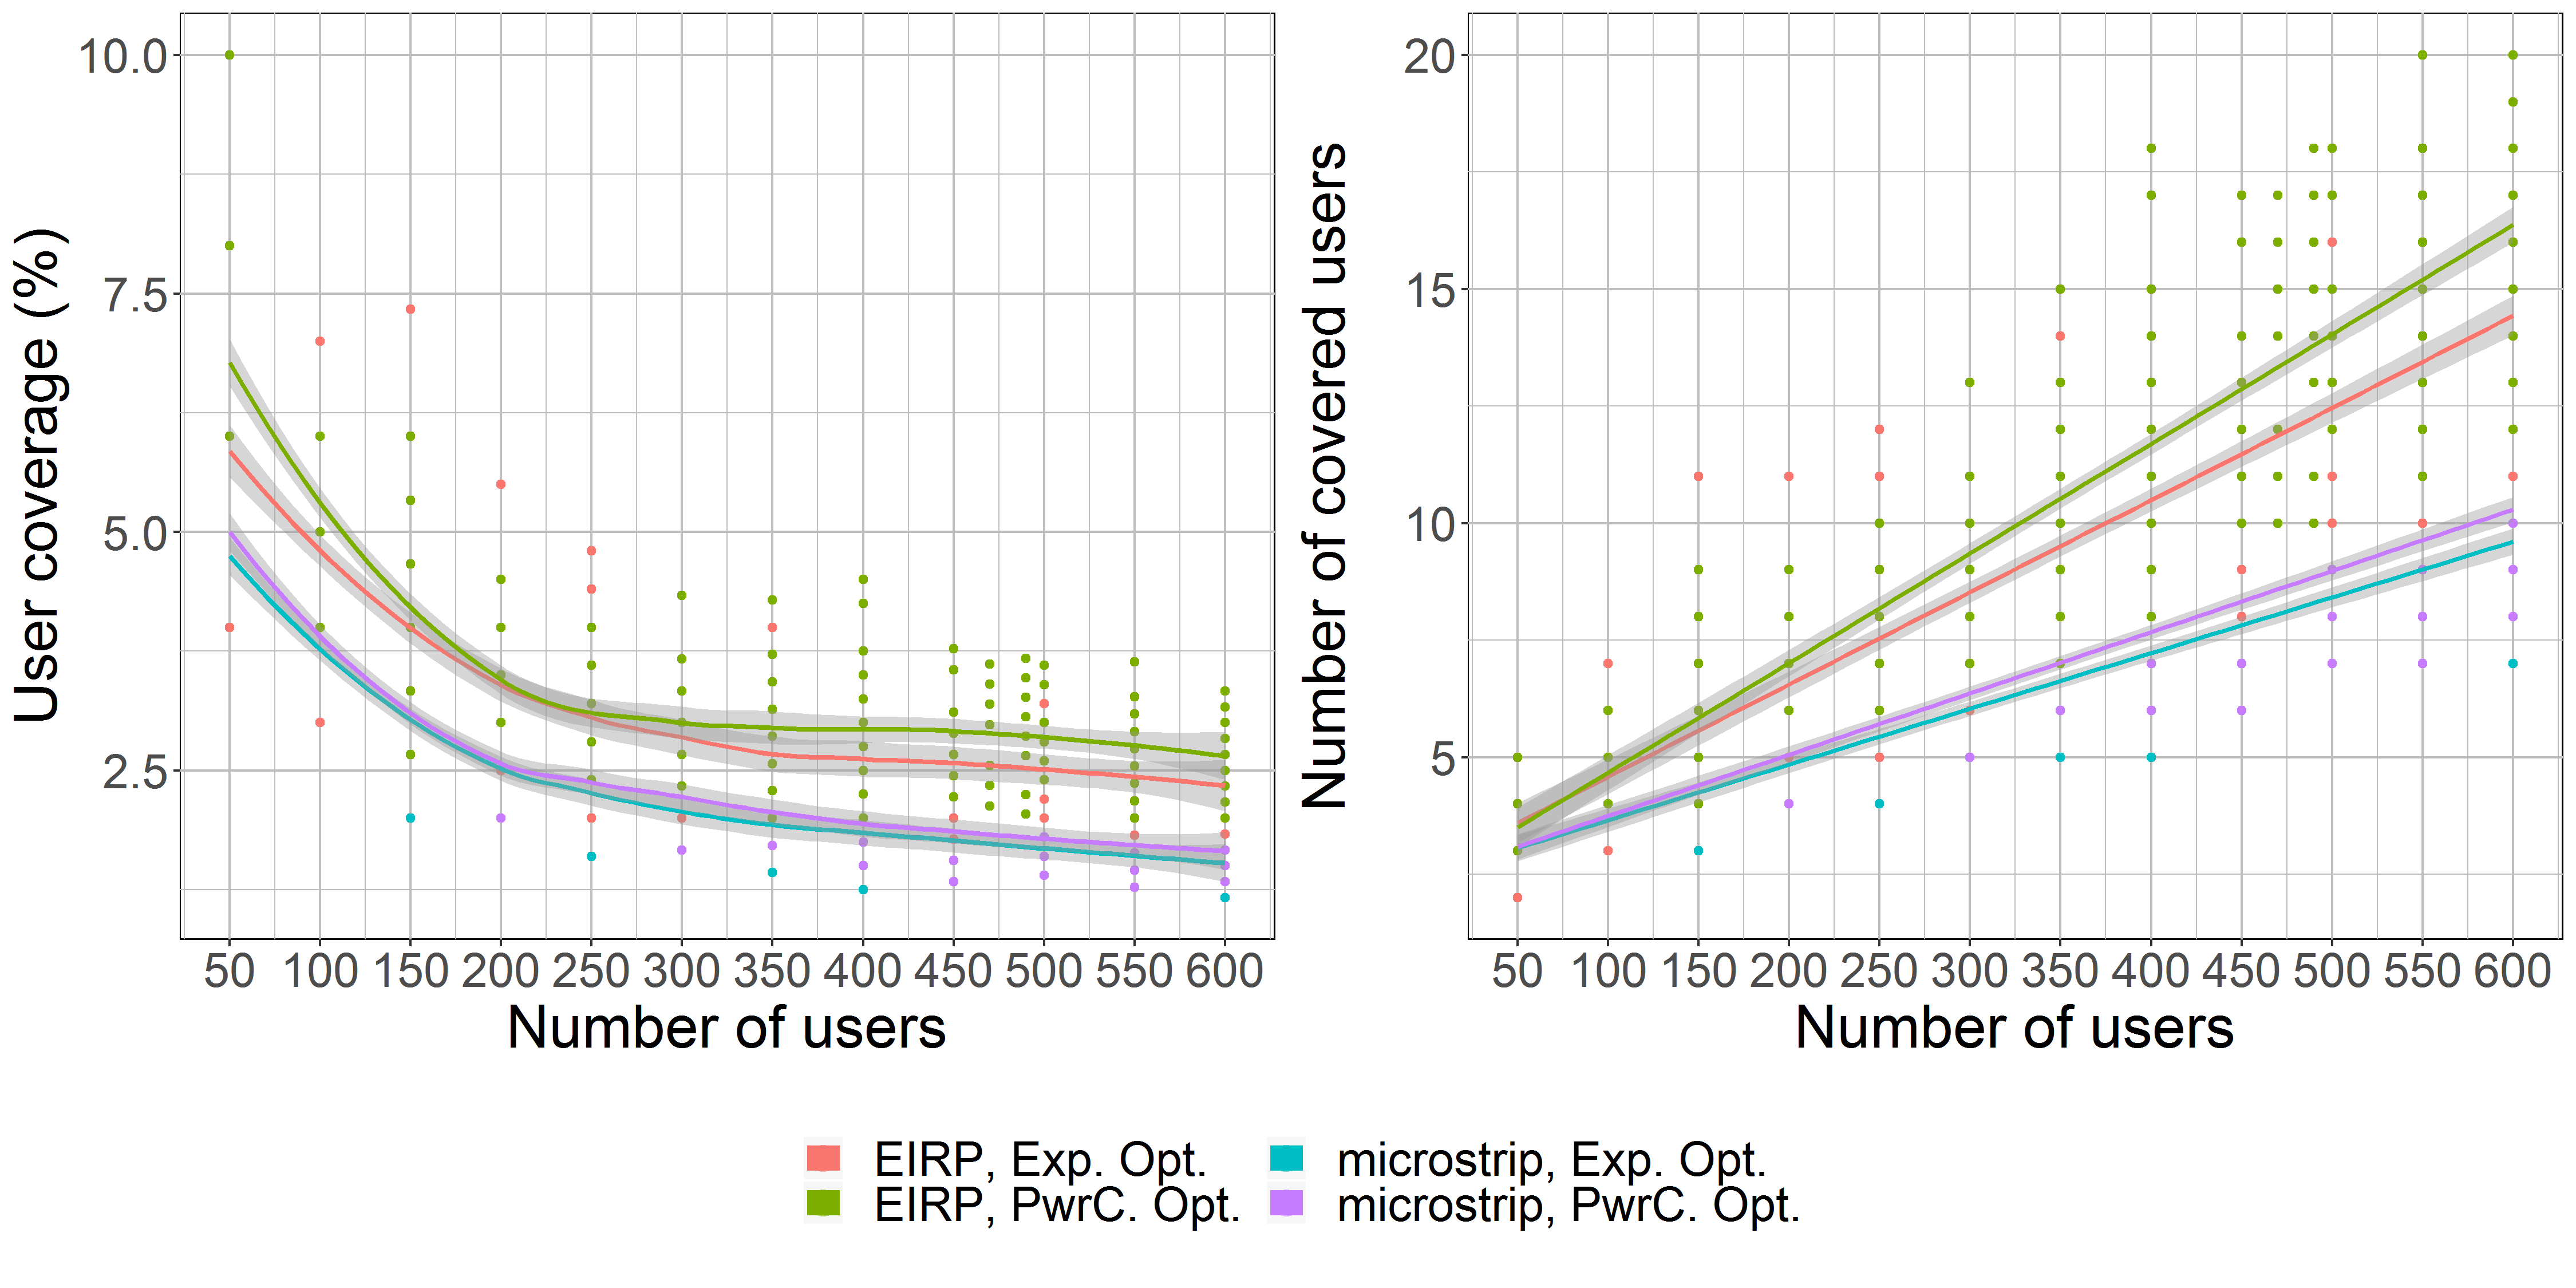
\includegraphics[width=\linewidth]{s2/uvsnumdronesAndCov.png}
  \caption{De invloed van de populatiegrootte op de dekkingsgraad.}
  \label{fig:s2uvsnumcovusers}
\end{figure}

Figuur  \ref{fig:s2b_dlAndPc}.a  is be\"invloed door \ref{fig:s2uvsnumcovusers}.a. 
de elektromagnetische straling neemt af wanneer minder gebruikers behandeld worden.
Bijvoorbeeld in een EIRP \gls{PwrC Opt} Netwerk met 50 gebruikers heeft 6,75\%
dekking wat overeenkomt met een gewogen gemiddelde blootstelling van 18 $mV/m$
Ter wel 600 gebruikers met een dekking van 2,75\% enkel maar 9 $mV/m$ geeft.
Verder is figuur \ref{fig:s2b_dlAndPc}.b rechtstreeks be\"invloed door figuur  \ref{fig:s2uvsnumcovusers}.b.
Wanneer de \gls{UABS} meer mensen behandeld neemt de kans op gebruikers met een ietwat slechter padverlies toe.
De  \gls{UABS} Zal dit probleem oplossen door het energieverbruik toe te laten nemen.
Zal dit probleem oplossen door het energieverbruik toe te laten nemen.
Een toenemende populatie van 50 naar 600 gebruikers zal het energieverbruik tussen 0,05 en 0,1 $W$ verhogen.
Voor dit scenario is geen duidelijk verschil te merken in energieverbruik tussen de vier verschillende configuraties.


\begin{figure}[h!]
  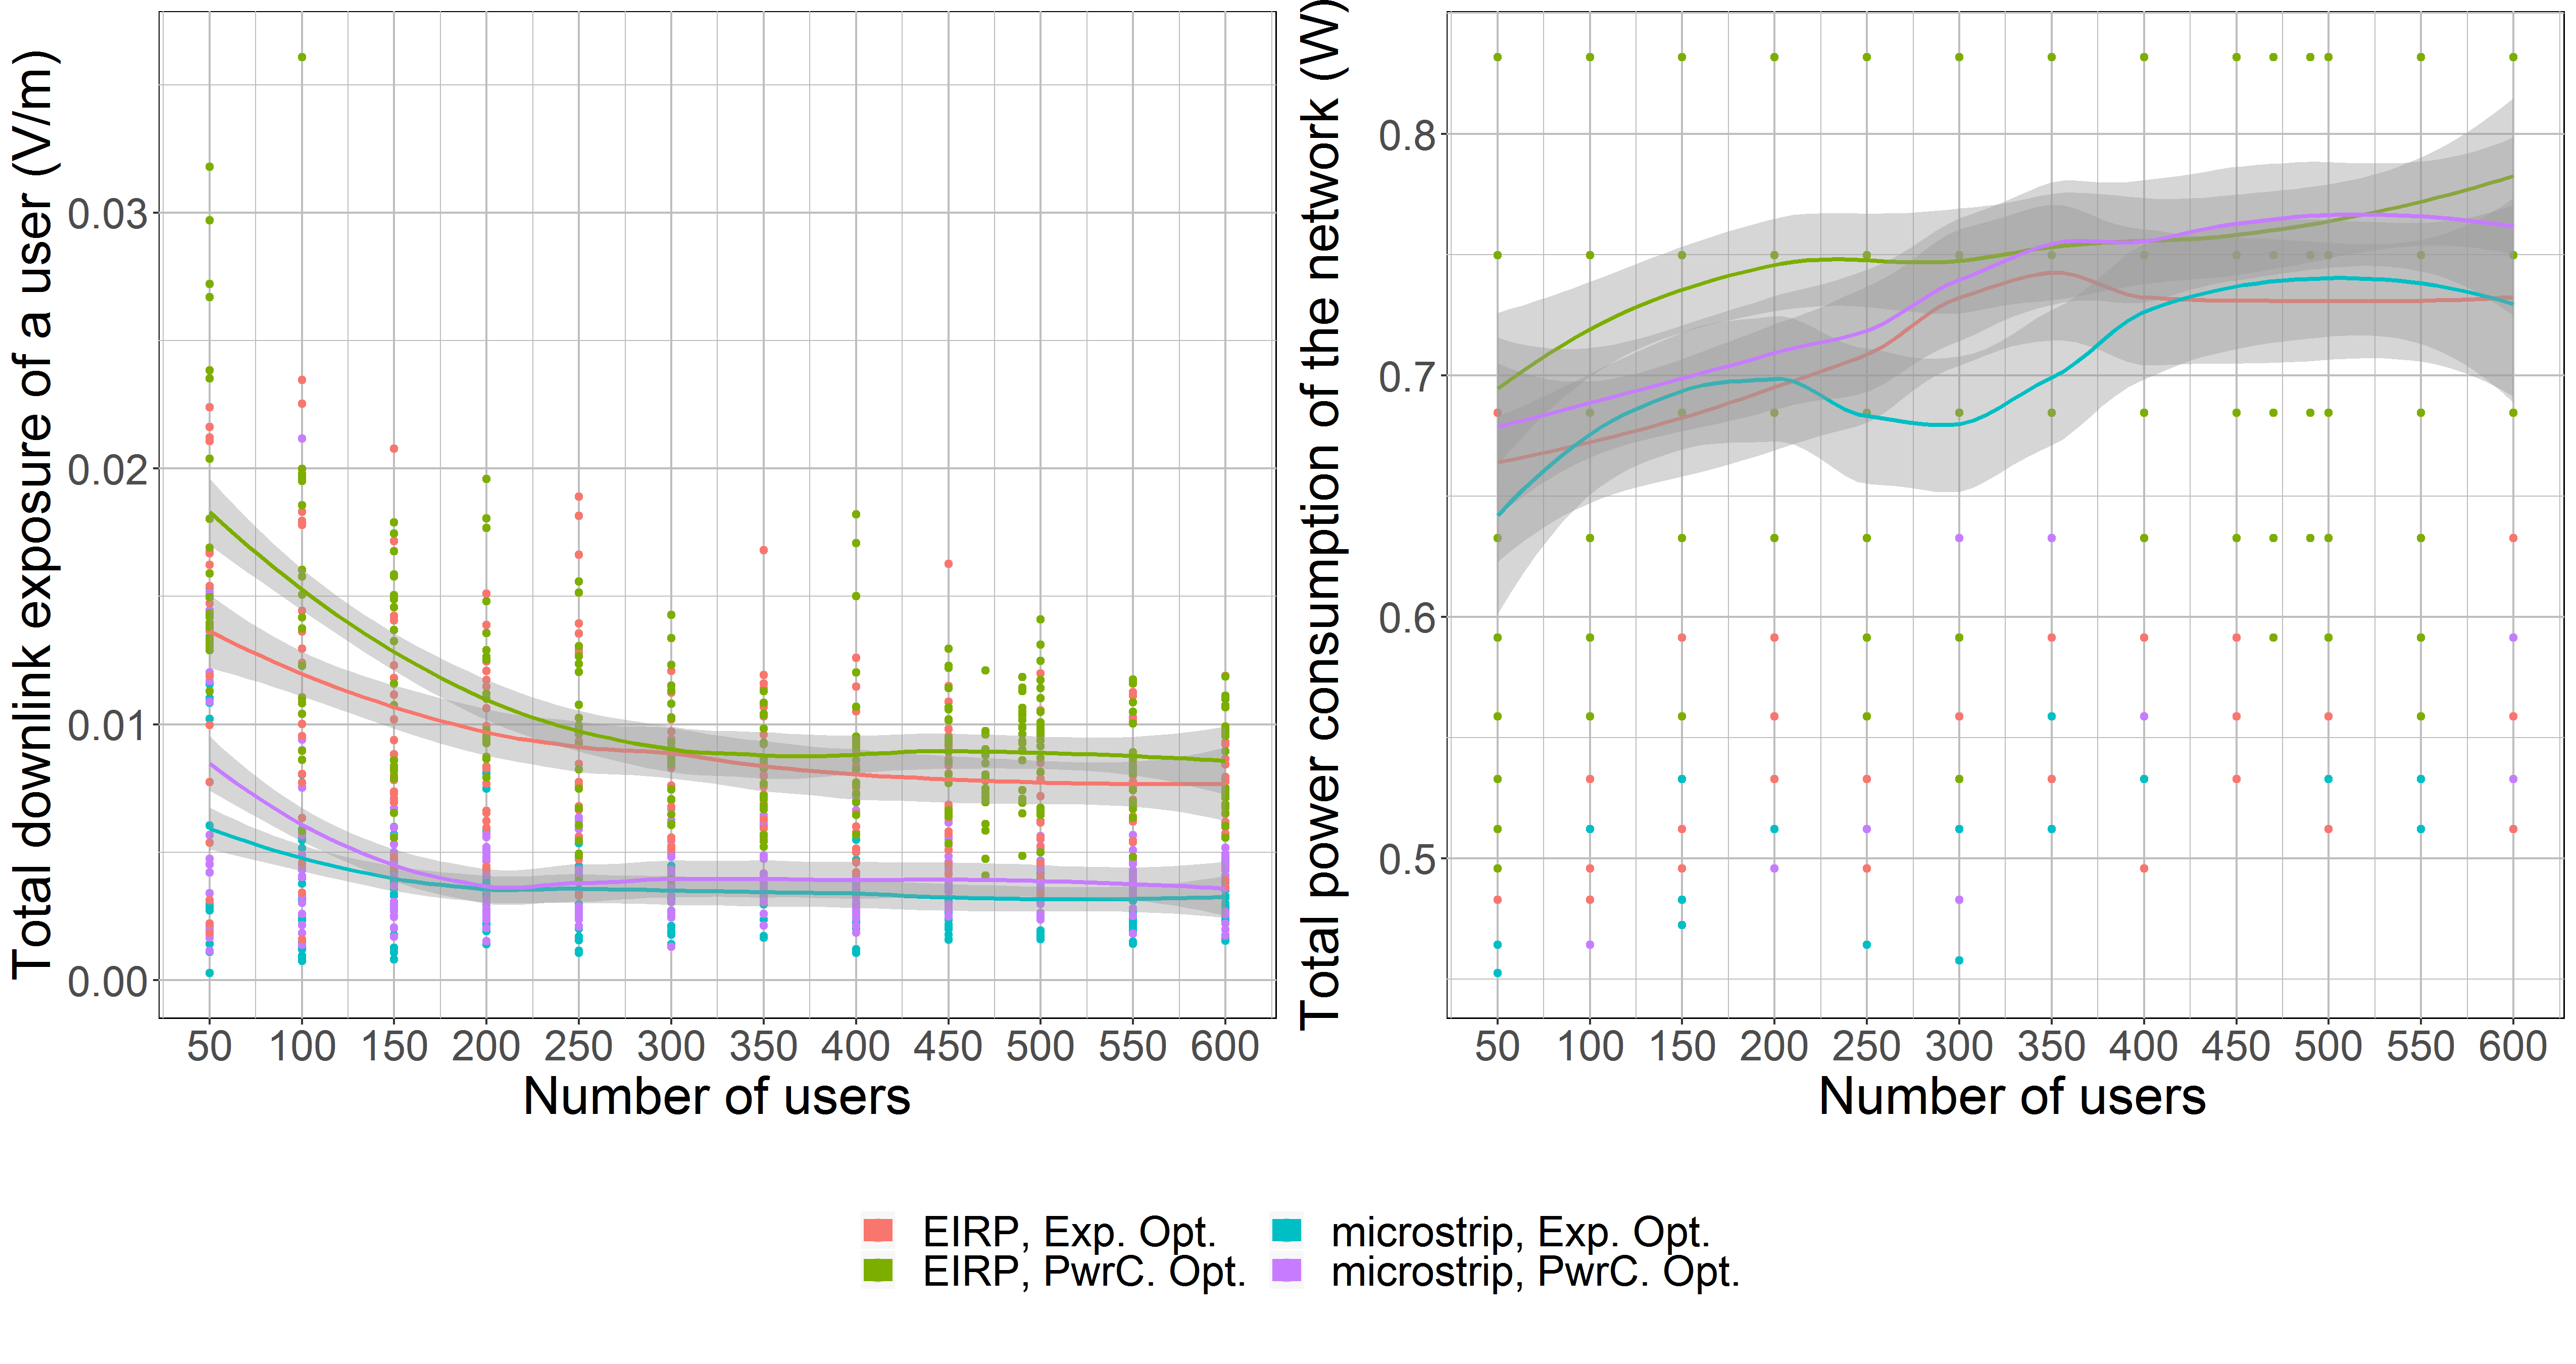
\includegraphics[width=\linewidth]{../results/s2/uvsdlAndPc.png}
  \caption{Deze twee figuren tonen hoe de verschillende populatiegrootte's invloed hebben op de \acs{DL} elektromagnetische straling (fig. a) en het energieverbruik (fig. b).}
  \label{fig:s2b_dlAndPc}
\end{figure}

De \gls{SAR} komende van de gebruikers zijn eigen apparaat is gemiddeld nul aangezien de meeste gebruikers niet behandeld worden.
Figuur \ref{fig:uvsulsarcentralUsers} toont de elektromagnetische blootstelling van de gedekte gebruiker juist onder de \gls{UABS}.
Scenario een toon de rits hoe de \gls{SAR} van de gebruiker zijn eigen mobiel apparaat enkel be\"invloed wordt door de vlieghoogte.
Dit wordt ook bevestigd door de resultaten in figuur  \ref{fig:uvsulsarcentralUsers} waar een constante 
$SAR^{myUE}$ van 0.15 $\mu W/kg$ gemeten wordt.
De \gls{SAR} van de  \gls{UABS} Onder had een kleine toename van 0,005  $\mu W/kg$.
Wanneer de populatie toeneemt zullen meer gebruikers dichtbij de \gls{UABS} terechtkomen.
De \gls{UABS} Zal waarschijnlijk beslissen om deze gebruiker ook te behandelen zoals zichtbaar is in figuur \ref{fig:connectionMap}.
Het is mogelijk dat deze gebruiker een slechter padverlies geeft door gebouwen of een ietwat grotere afstand. Hierdoor zal de
\gls{DL} \gls{SAR} van de gebruiker onder de drone toenemen.
De elektromagnetische straling's van andere personen een mobiel apparaat is heel laag zoals 
reeds vermeld en is daarom apart toegevoegd in figuur  \ref{fig:uvsulsarcentralUsers}.b.
De figuur toont hoe de \gls{SAR} van andere mobiele apparaten toeneemt van nul tot $0,15\ pW/kg$.


\begin{figure}[h]
\subfloat[50 gebruikers]{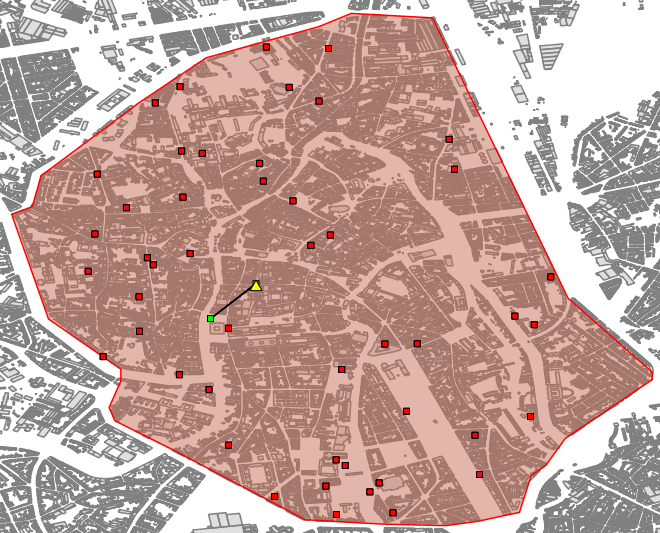
\includegraphics[width=0.49\linewidth]{../images/connectionsMap50Users.png}}
\hfill
\subfloat[600 gebruikers]{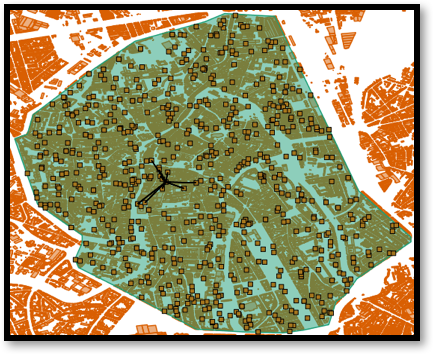
\includegraphics[width=0.49\linewidth]{../images/connectionsMap600Users.png}}
\caption{ Overzicht van welke gebruikers verbonden zijn met de \acs{UABS}.}
  \label{fig:connectionMap}
\end{figure}

\begin{figure}[h]
\centering
  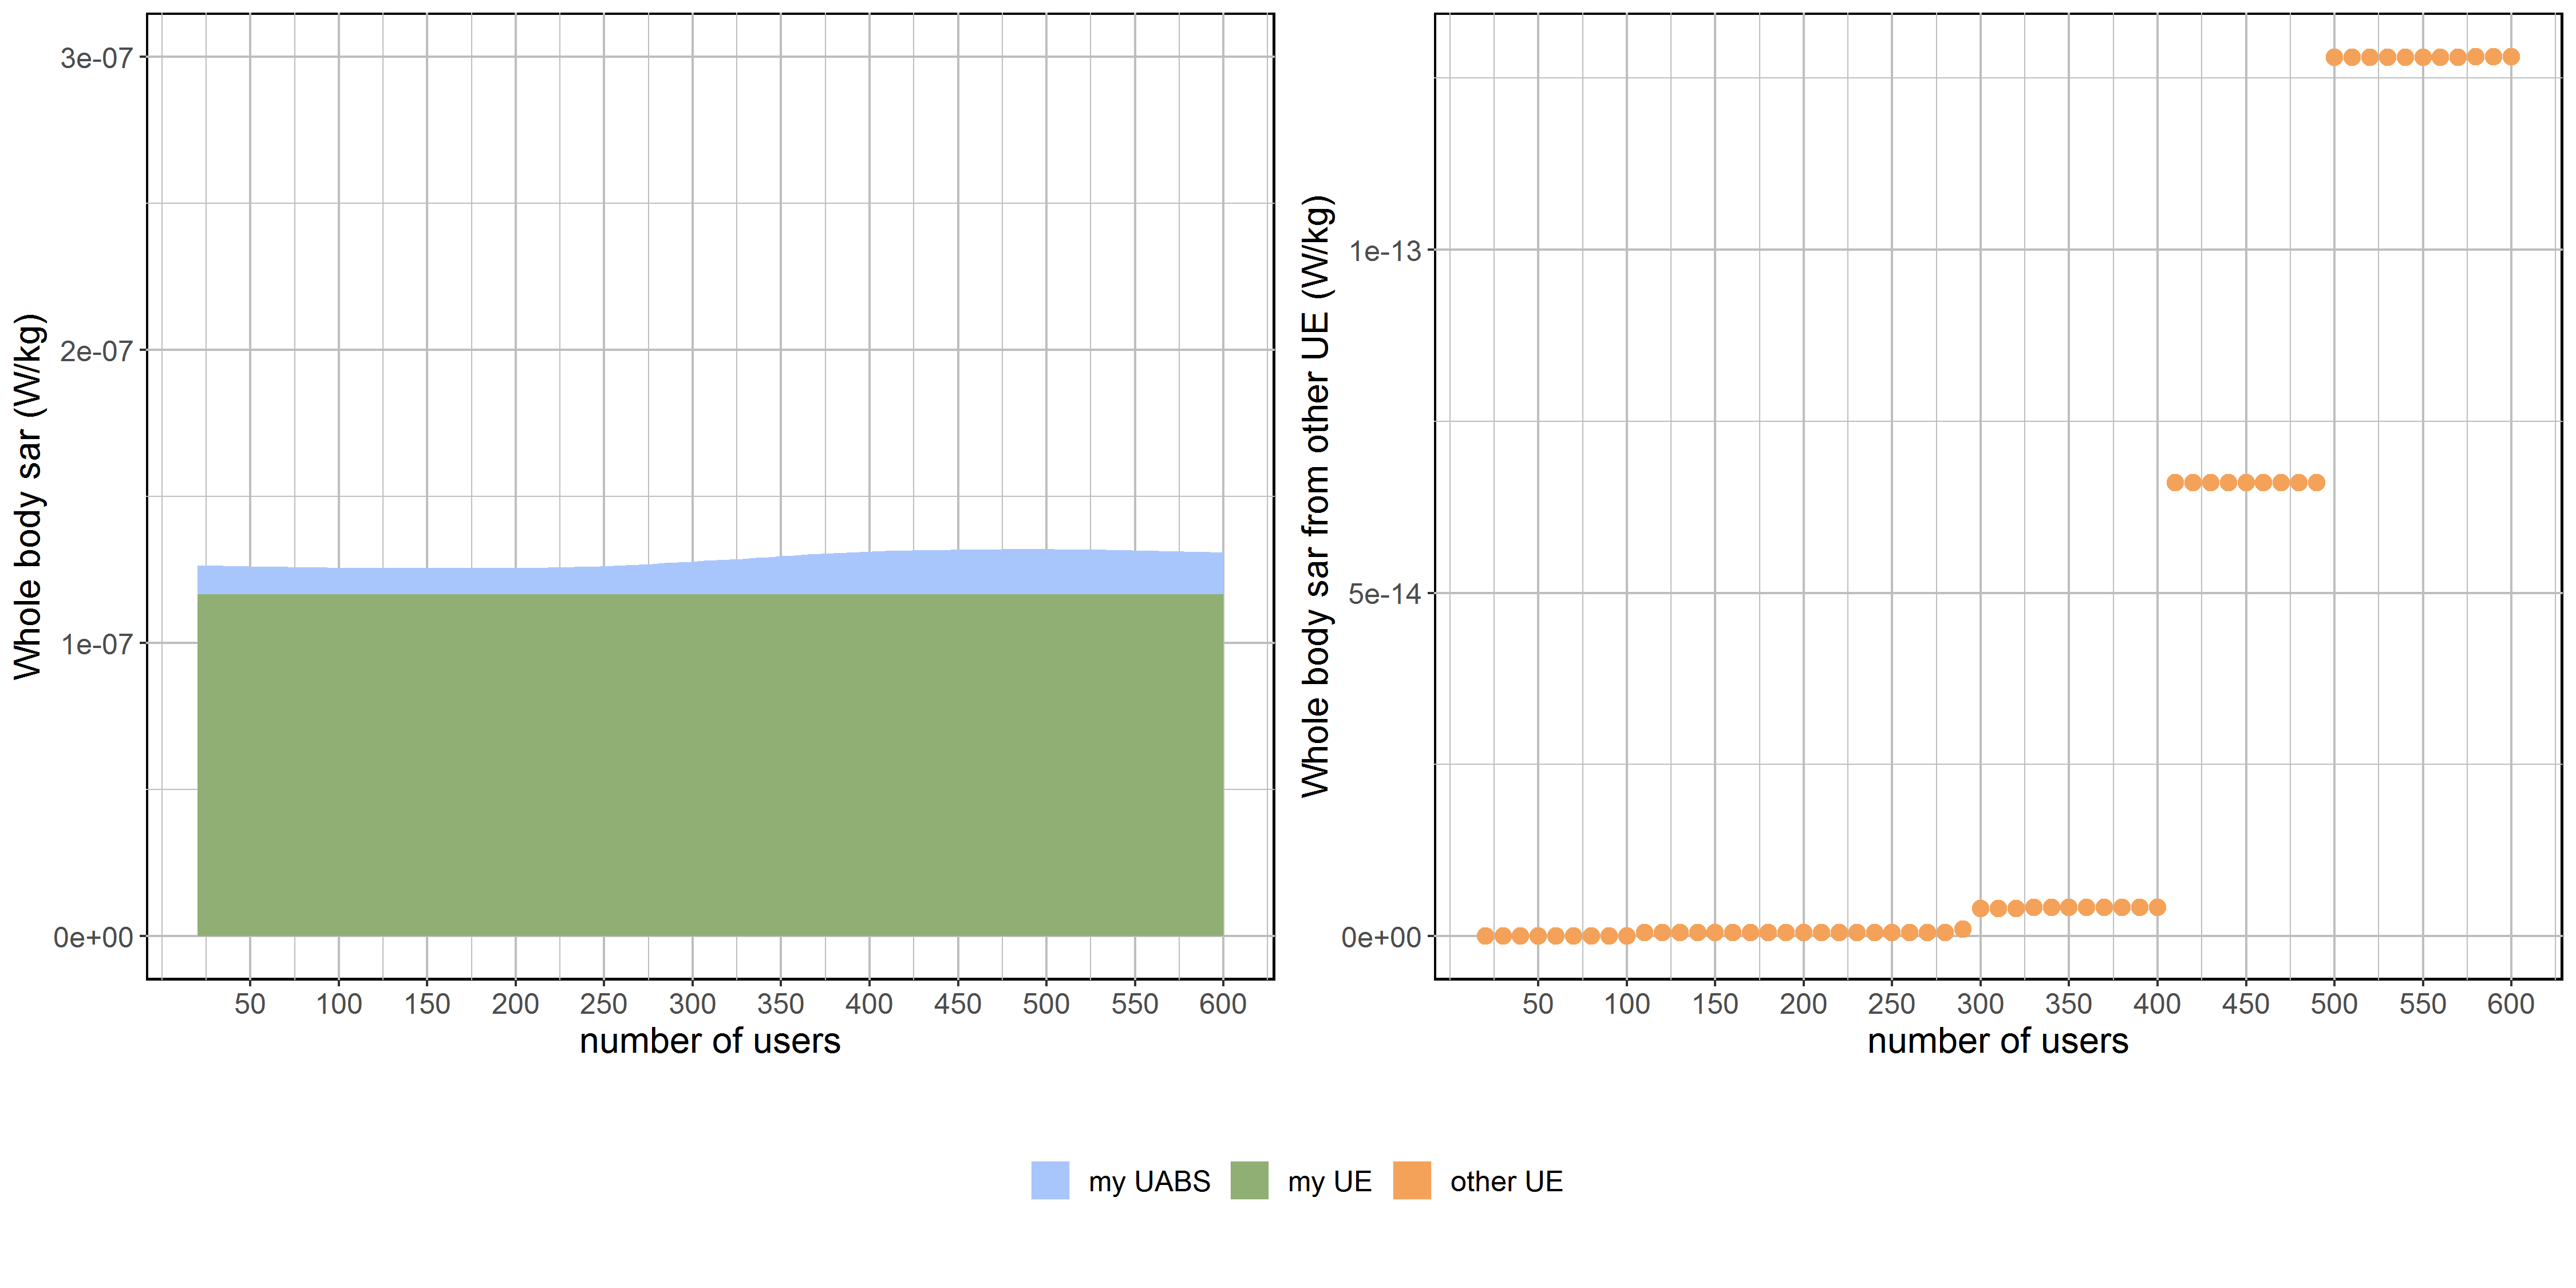
\includegraphics[width=0.9\linewidth]{../results/s2/uvsulsarcentralUser.png}
  \caption{SAR-waarden voor de gebruiker die zich onder de \acs{UABS} bevindt.}
  \label{fig:uvsulsarcentralUsers}
\end{figure}

\subsection{Ongelimiteerd aantal \gls{UABS}'s}
\subsubsection{Variabele vlieghoogte}
Hetzelfde scenario als in de voorgaande sectie wordt hier onderzocht. Enkel is er hier een ongelimiteerd aantal 
\gls{UABS}'s beschikbaar. De resultaten bewijzen dat de verschillende optimalisatiestrategie\"en werken zoals bedoeld.
Een \gls{PwrC Opt} heeft inderdaad een lager energieverbruik maar dit komt ten koste van een hogere elektromagnetische straling.
Aan de andere kant zal een  \gls{Exp Opt} netwerk de elektromagnetische blootstelling reduceren door meer drones te gebruiken waardoor tevens 
het energieverbruik zal toenemen. Deze conclusie werd reeds gemaakt in \cite{J1} en is bevestigd door deze resultaten.
Bijvoorbeeld bij het vergelijken van beide optimalisatiestrategieën zal voor dezelfde
\gls{isotropicradiator} en dezelfde standaard vlieghoogte Een energiezuinig netwerk 51 $W$ 
en de gebruikers blootstellen aan $15\ mV/m$.
Wanneer optimaliseert wordt naar elektromagnetische straling's zal de blootstelling zakken naar 
$11.5\ mV/m$ wat ten koste komt van een hoger energieverbruik van $54\ W$.


\begin{figure}[h!]
  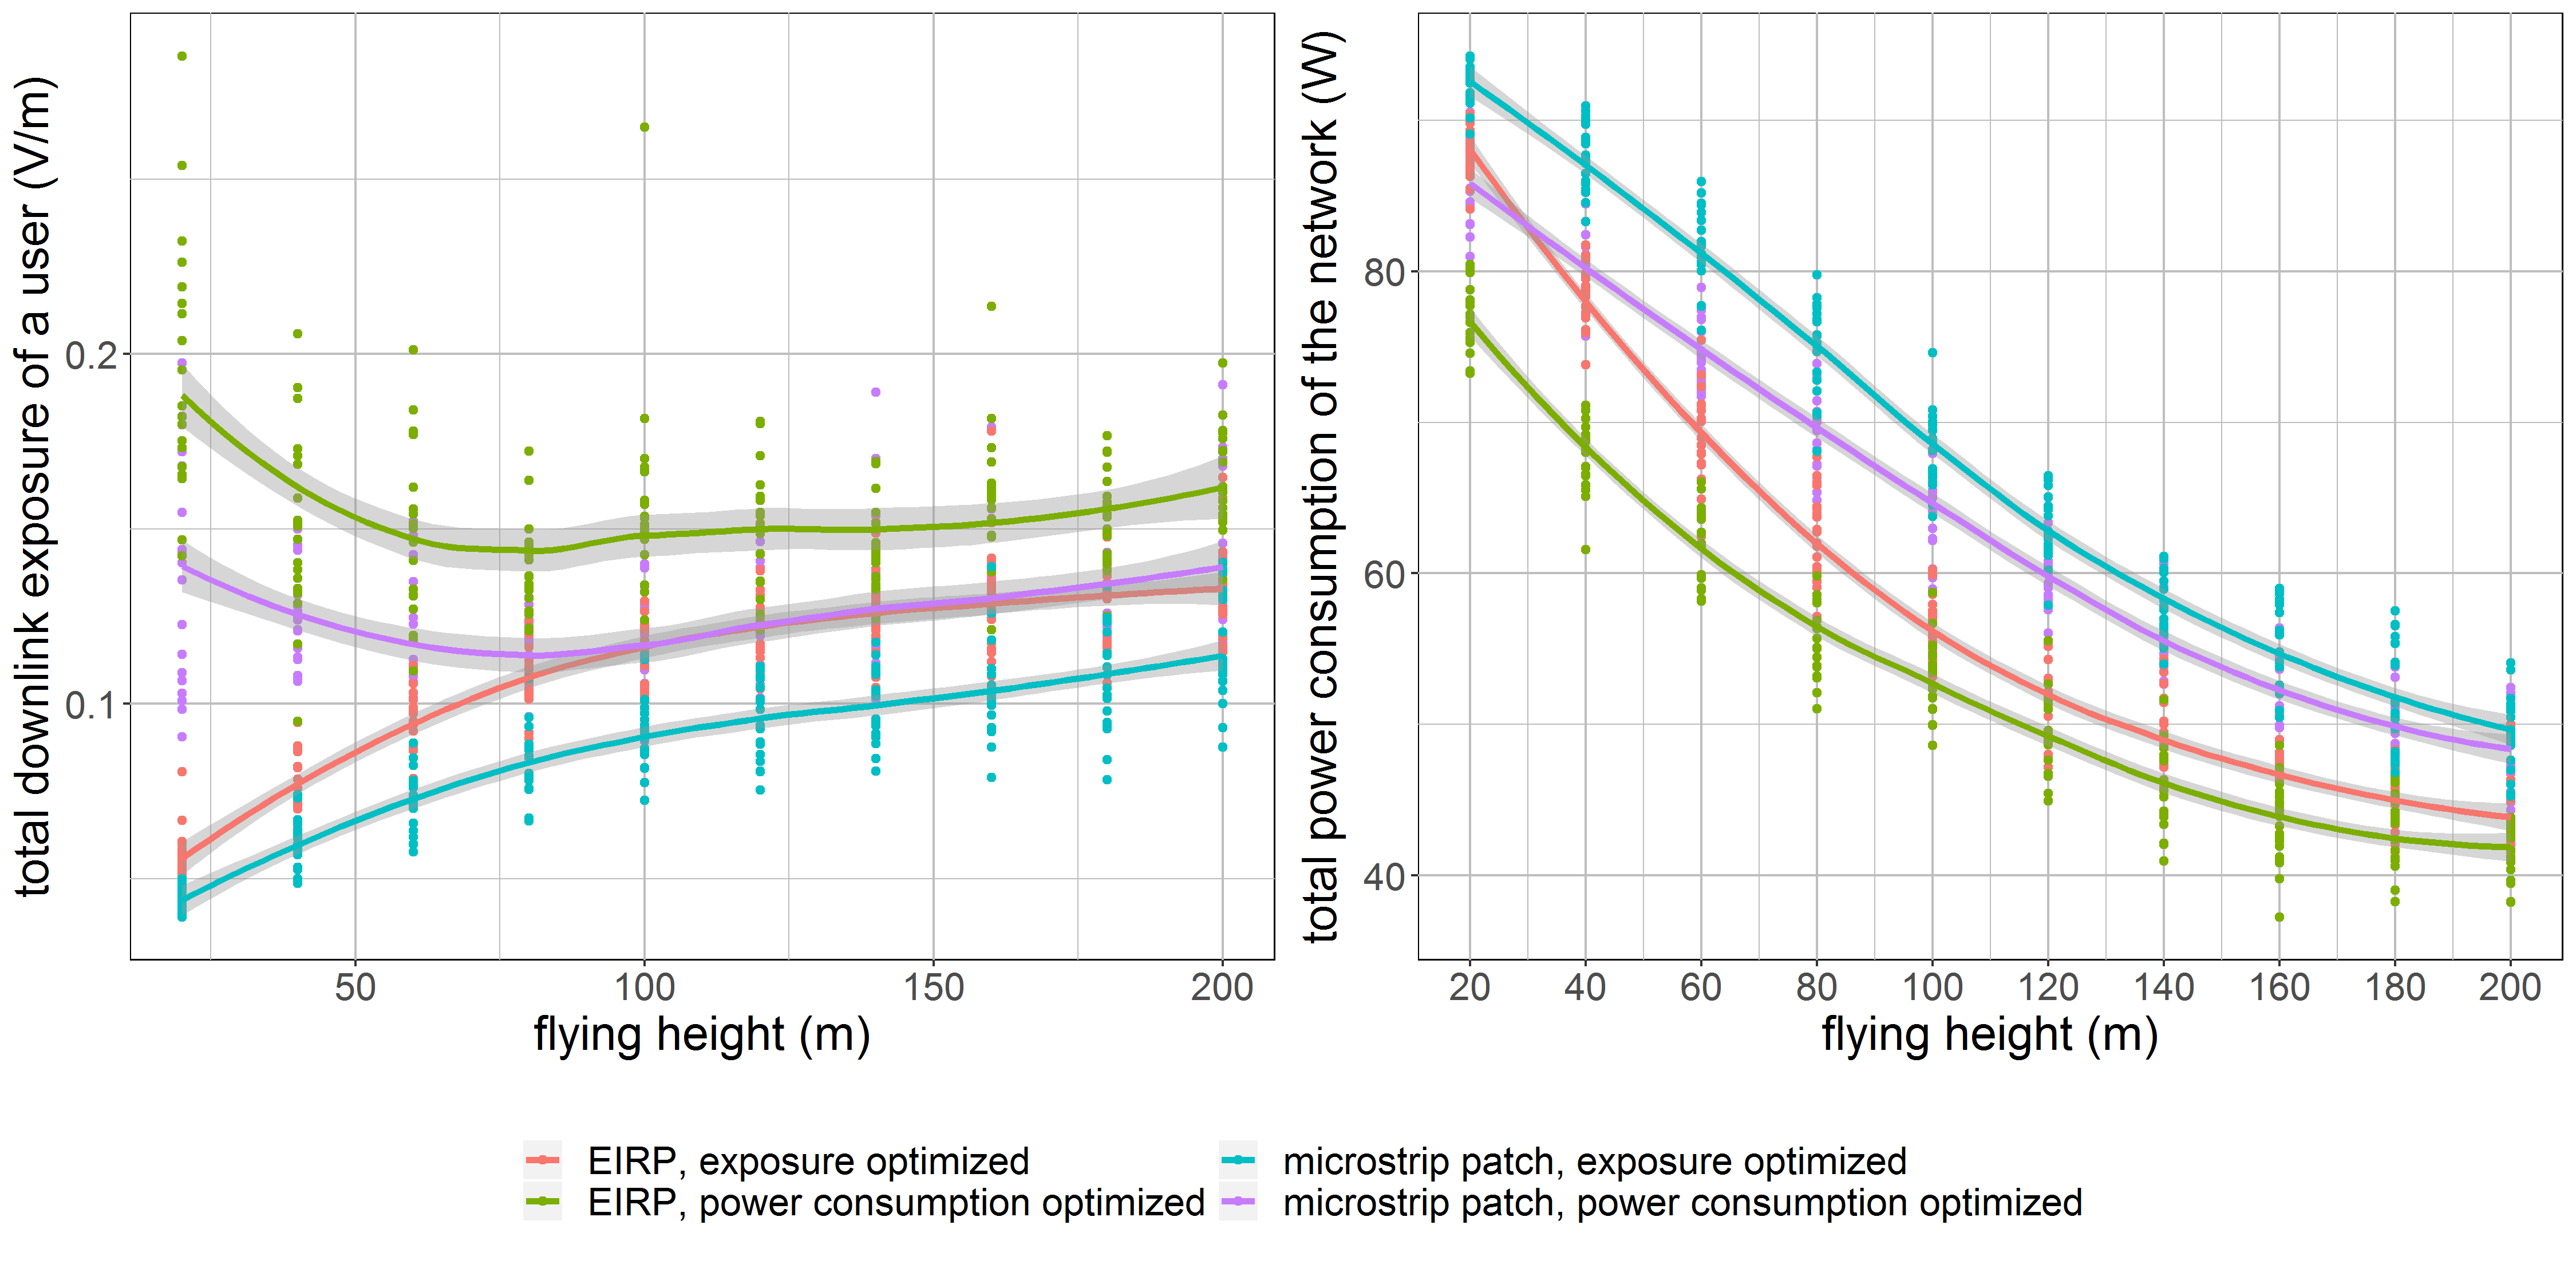
\includegraphics[width=\linewidth]{../results/s3/fhvsdlAndPc.png}
  \caption{Deze twee figuren tonen hoe de vlieghoogte invloed heeft op de \acs{DL} elektromagnetische straling (fig. a) en het energieverbruik (fig. b).}
  \label{fig:s3a_dlAndPc}
\end{figure}

De elektromagnetische blootstelling in figuur \ref{fig:s3a_dlAndPc} toont een logaritmische toename bij een 
\gls{Exp Opt} netwerk terwijl een \gls{PwrC Opt} netwerk eerder een concaaf verband met de vlieghooghte weergeeft 
waarbij het laagste punt zich op 70 meter bevindt.

Figuur \ref{fig:s3a_numDronesAndCov}.a Toont dat een optimale dekking van 90\% bereikt wordt bij een lagere vlieghoogte van 40 m.
Hier is echter een nadeel aan verbonden. 
Figuur \ref{fig:s3a_numDronesAndCov}.b 
toont dat het aantal vereiste droens toeneemt wanneer de vlieghoogte lager wordt; 
een vaststelling die reeds gemaakt is in \cite{J2}.
Bijvoorbeeld, een microstrip \gls{Exp Opt} netwerk en een \gls{EIRP} \gls{PwrC Opt} netwerk 
Vereisen respectievelijk 84 en 64 drones op een vlieghoogte van 200 m wat respectievelijk toeneemt naar 
211 en 162 drones met een veel lagere vlieghoogte van 20 m.

\begin{figure}[]
  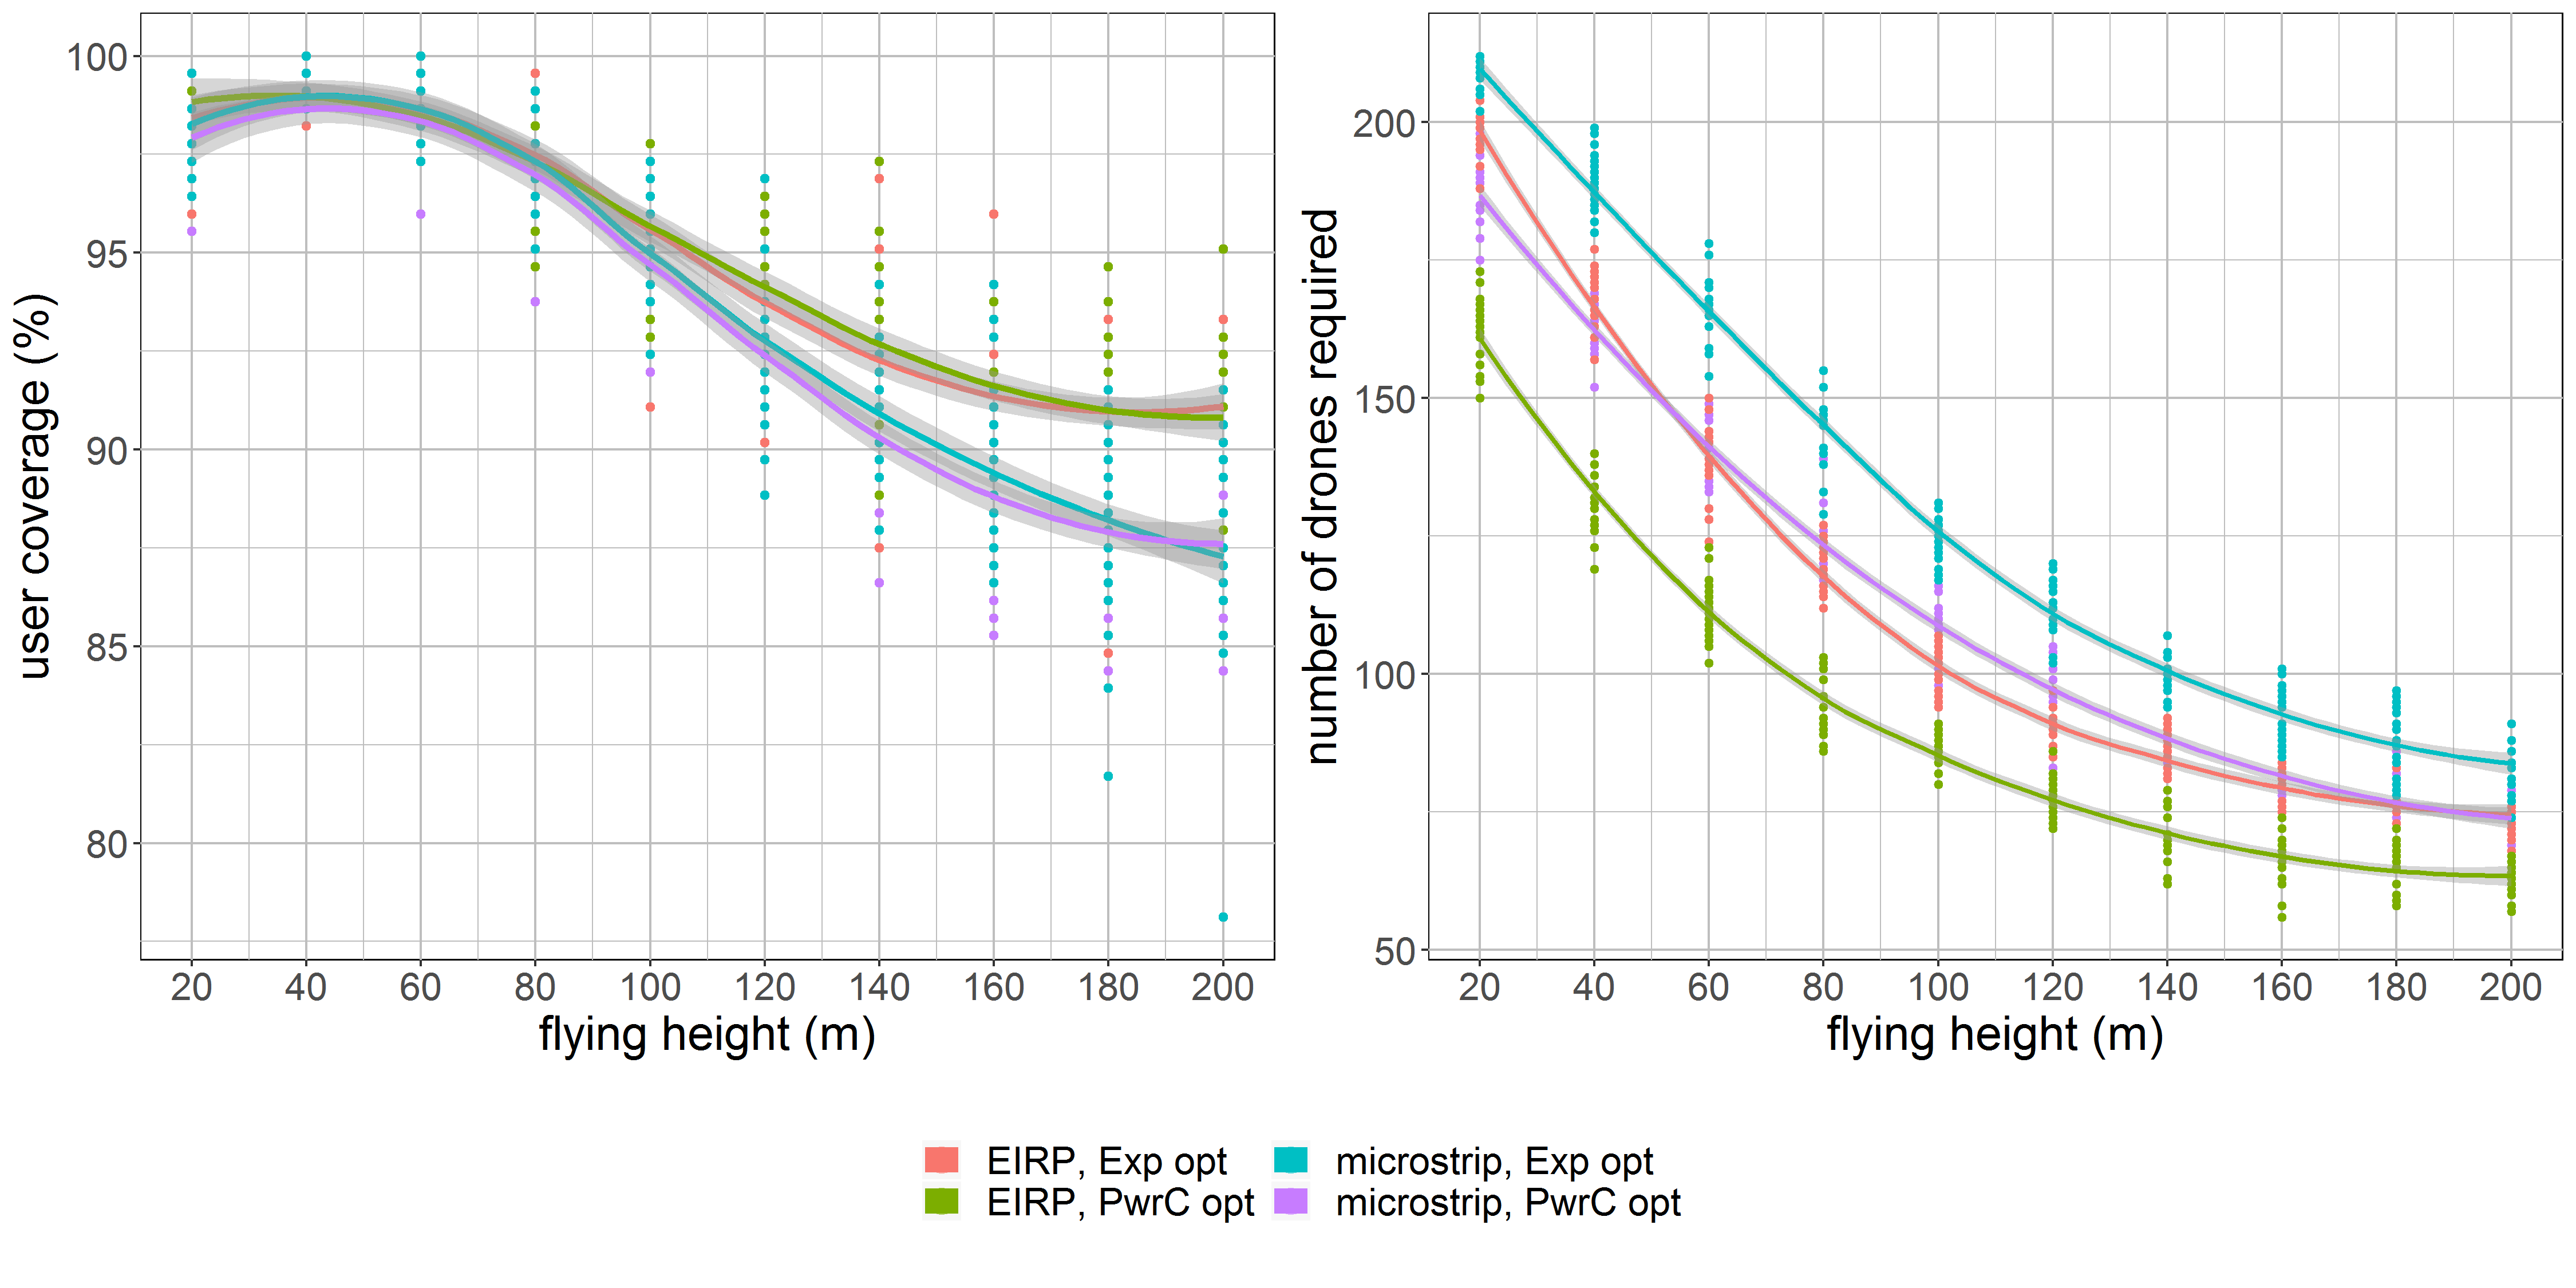
\includegraphics[width=\linewidth]{../results/s3/fhvsnumdronesAndCov.png}
  \caption{Deze grafiek toont hoeveel drones vereist zijn op verschillende vlieghoogte's terwijl er getracht wordt om 100\% dekking te bereiken.}
  \label{fig:s3a_numDronesAndCov}
\end{figure}

Figuur \ref{fig:s3a_fourSourcesMatrix} Stond de bijdragen van elke bron aan de totale \gls{SAR}.
Het eerste  gevolg van de vlieghoogte te laten toenemen van 20 naar 200 m is de 
toenemende  \gls{SAR}  van de gebruiker zijn eigen gsm dewelke varieert tussen 89 en 141 $nW/kg$;
een gedraag dat reeds geconstateerd werd in het eerste scenario.
Figuur \ref{fig:s3a_fourSourcesMatrix} toont aan dat de vlieghooghte hoger wordt dan de \gls{NLOS} van de gebouwen 
rond 70 tot 80 meter. Hierna blijft de \gls{SAR} van de behandel \gls{UABS} min of meer gelijk voor alle configuraties.
De $SAR^{myUABS}$ varieert voor deze hogere vlieghoogte's tussen
 $160\ nW/kg$ voor een microstrip \gls{PwrC Opt} netwerks en rond $98\ nW/kg$ voor een microstrip \gls{Exp Opt} en \gls{EIRP} \gls{PwrC Opt} netwerken.
De \gls{EIRP} \gls{Exp Opt} netwerk is bevindt zich rond $47\ nW/kg$.
Deze gore vliegen hoor dus zullen ook resulteren in een toegenomen elektromagnetische straling's van andere
\gls{UABS}'s.
Wanneer de vlieghoogte toeneemt van 20 tot 200 m zal de $SAR^{otherUABS}$ tussen 115 en 140
$nW/kg$ voor \gls{EIRP} antennes bedragen en tussen 54 en 74 $nW/kg$ voor microstrip patch antennes.
Dit voorbij de optimalisatiestrategie\"en.


\begin{figure}[h!]
  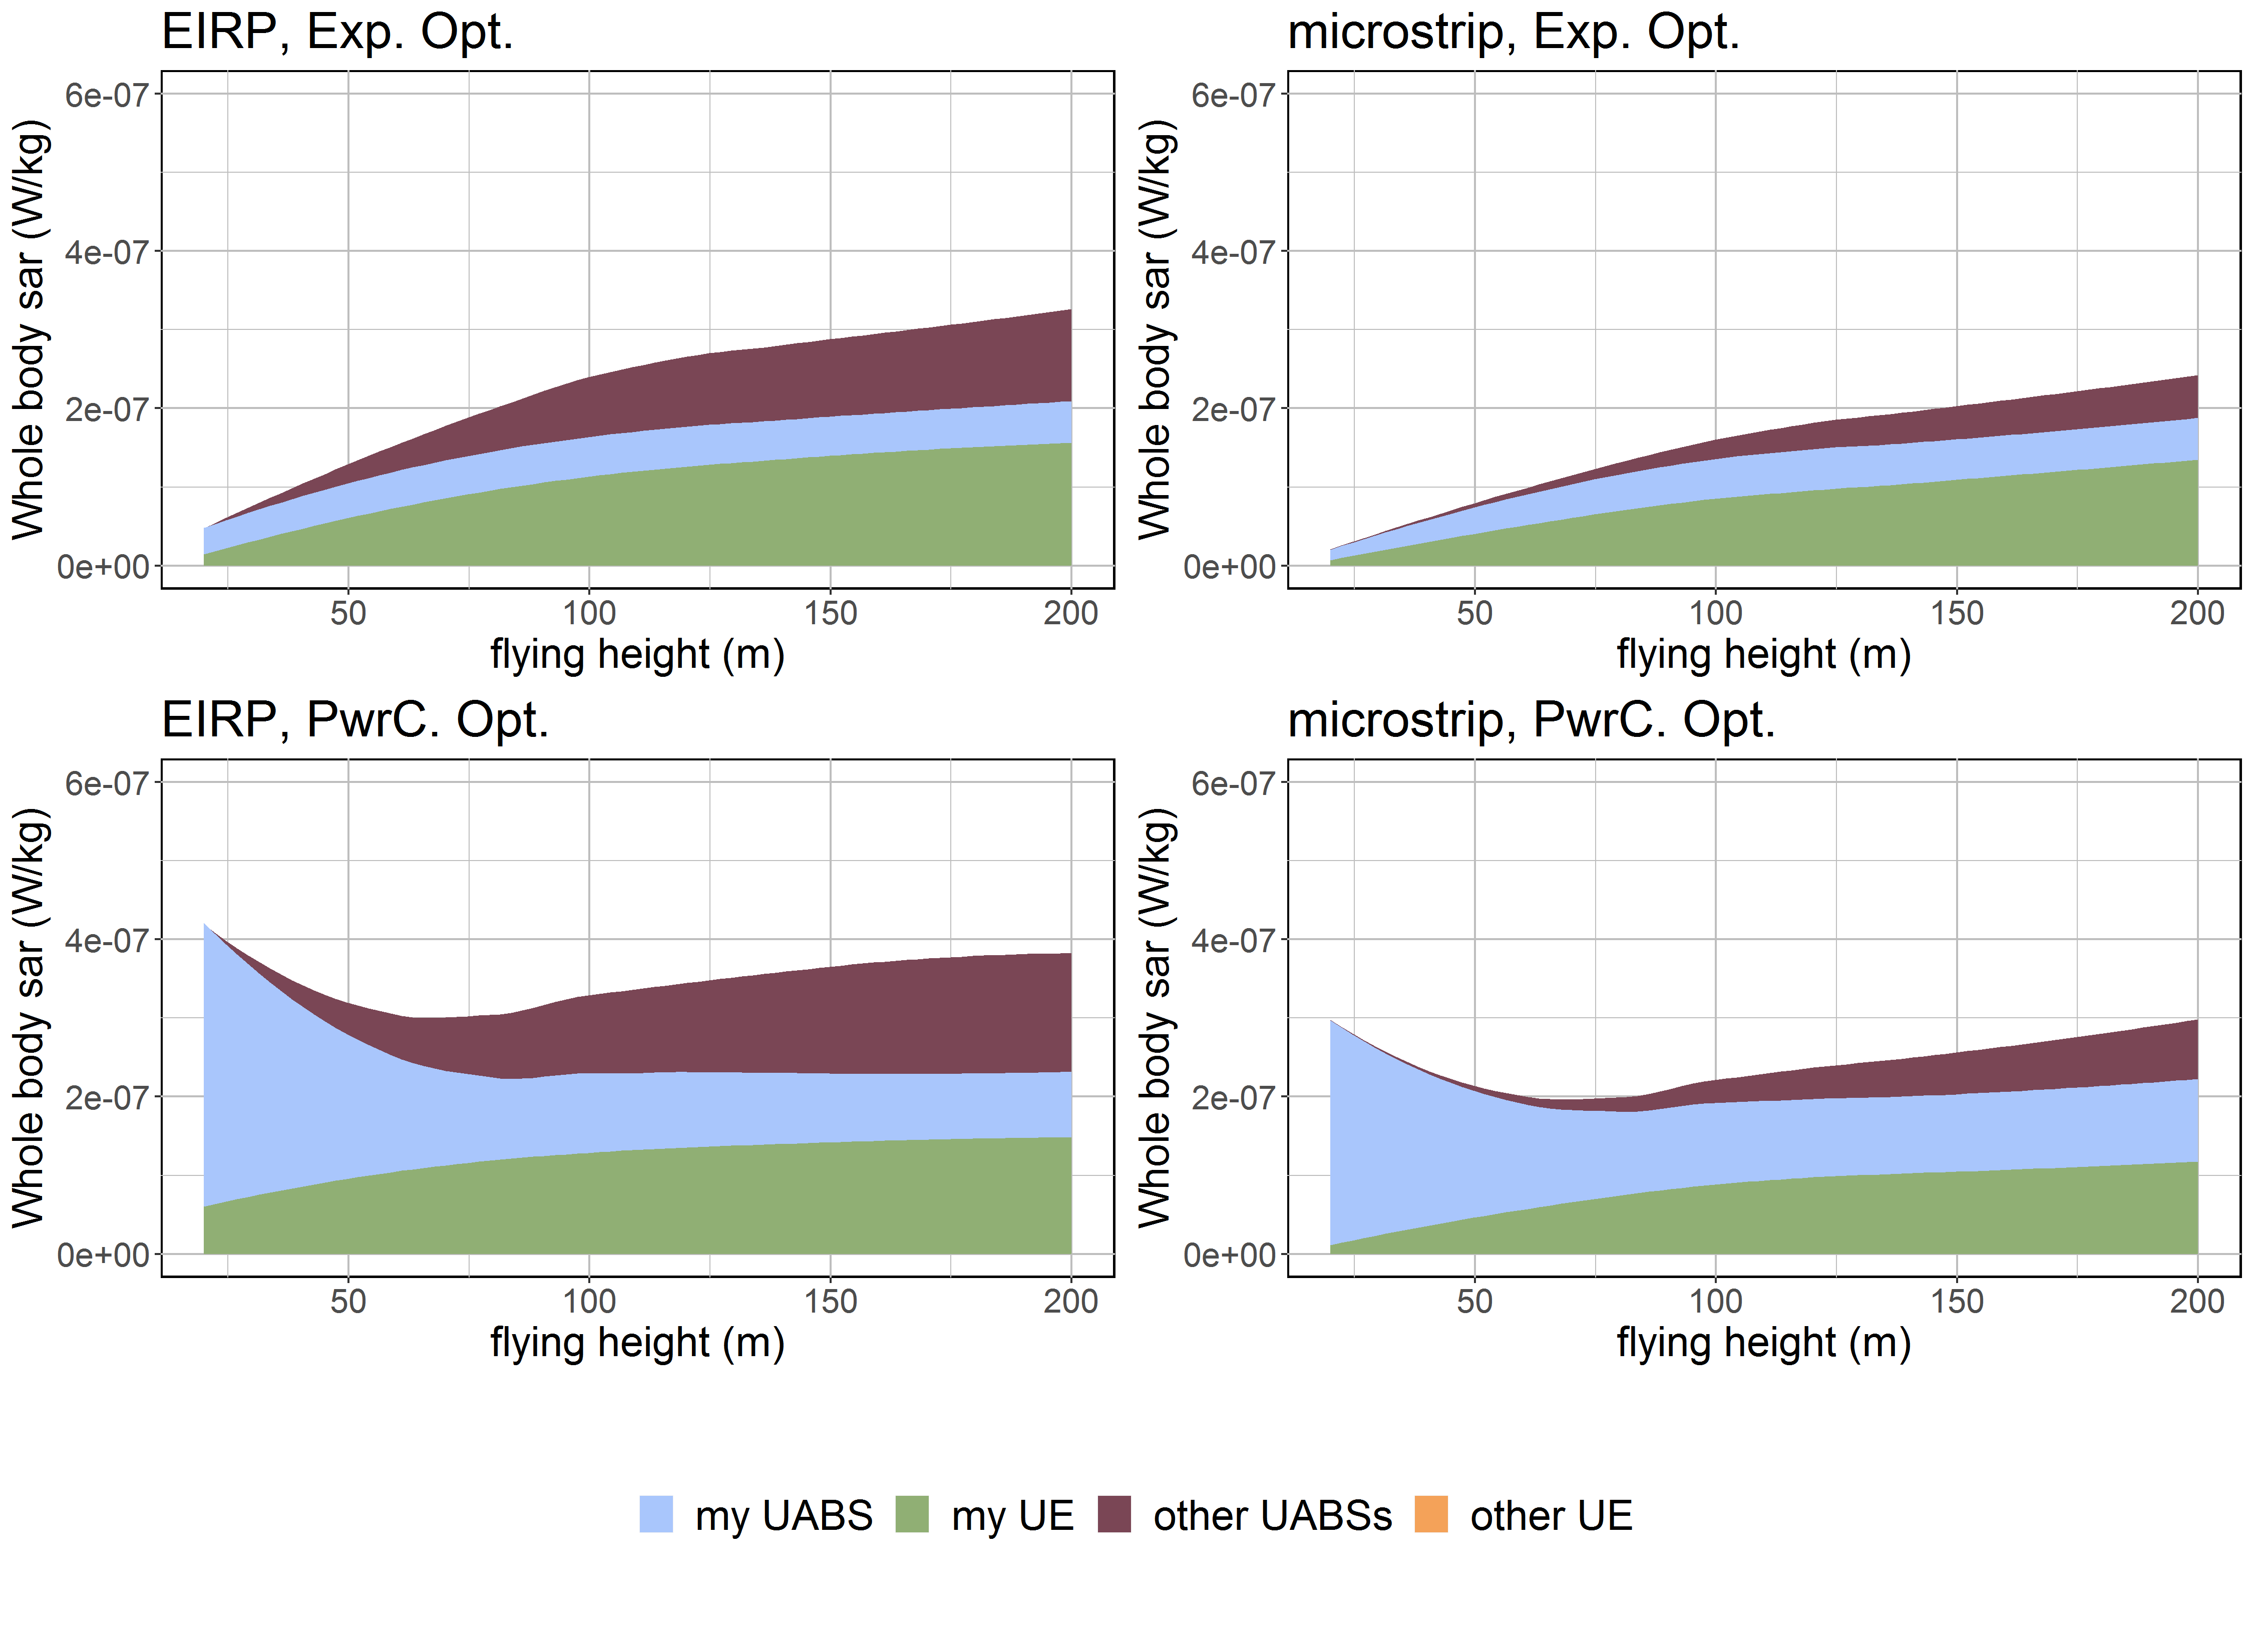
\includegraphics[width=\linewidth]{../results/s3/fhFourSources.png}
  \caption{Elke grafiek komt overeen met een van de vier mogelijke configuraties.
   De bijdrage van elke bron aan de totale \acs{SAR} is voor een variërende vlieghoogte.}
  \label{fig:s3a_fourSourcesMatrix}
\end{figure}

\subsubsection{Variabele aantal gebruikers}
De tweede onderzochte parameter van dit scenario is een vari\"rende populatiegrootte
terwijl de vlieghoogte zich op 100 m zal bevinden.
Figuur  \ref{fig:s3b_numdronesAndCov}.a toont hoe de tool tracht 100\% dekking te bereiken.
Dit percentage van het dikte personen is iets wat minder voor kleinere netwerken. 
Voor slechts 50 personen zal de gemiddelde dekking
Zich rond 93\% bevinden terwijl een netwerk van 600 personen en dekking van 97\% heeft.
Figuur \ref{fig:s3b_numdronesAndCov}.b toont aan dat meer \gls{UABS}'s  vereist zijn voor grotere populaties.
Het verschil in optimalisatie strategie is heel, miniem voor kleine netwerken maar neemt snel toe. 
Wanneer de populatie groeit van 50 tot 600 gebruikers zullen 200 \gls{UABS}'s ik extra vereist zijn bij een
 microstrip \gls{Exp Opt} netwerk,
 rond 130 extra \gls{UABS}'s voor een \gls{EIRP} \gls{Exp Opt} netwerk of een microstrip \gls{PwrC Opt} netwerk
 en 110 extra \gls{UABS}'s voor een \gls{EIRP} \gls{PwrC Opt} netwerk.
Dit is een verwacht gedrag wanneer er gekeken wordt naar het voorgaande scenario waarbij,
 met slechts \'e\'en \gls{UABS}, het percentage van behandelde gebruikers afnam voor grotere populaties.



\begin{figure}[h]
  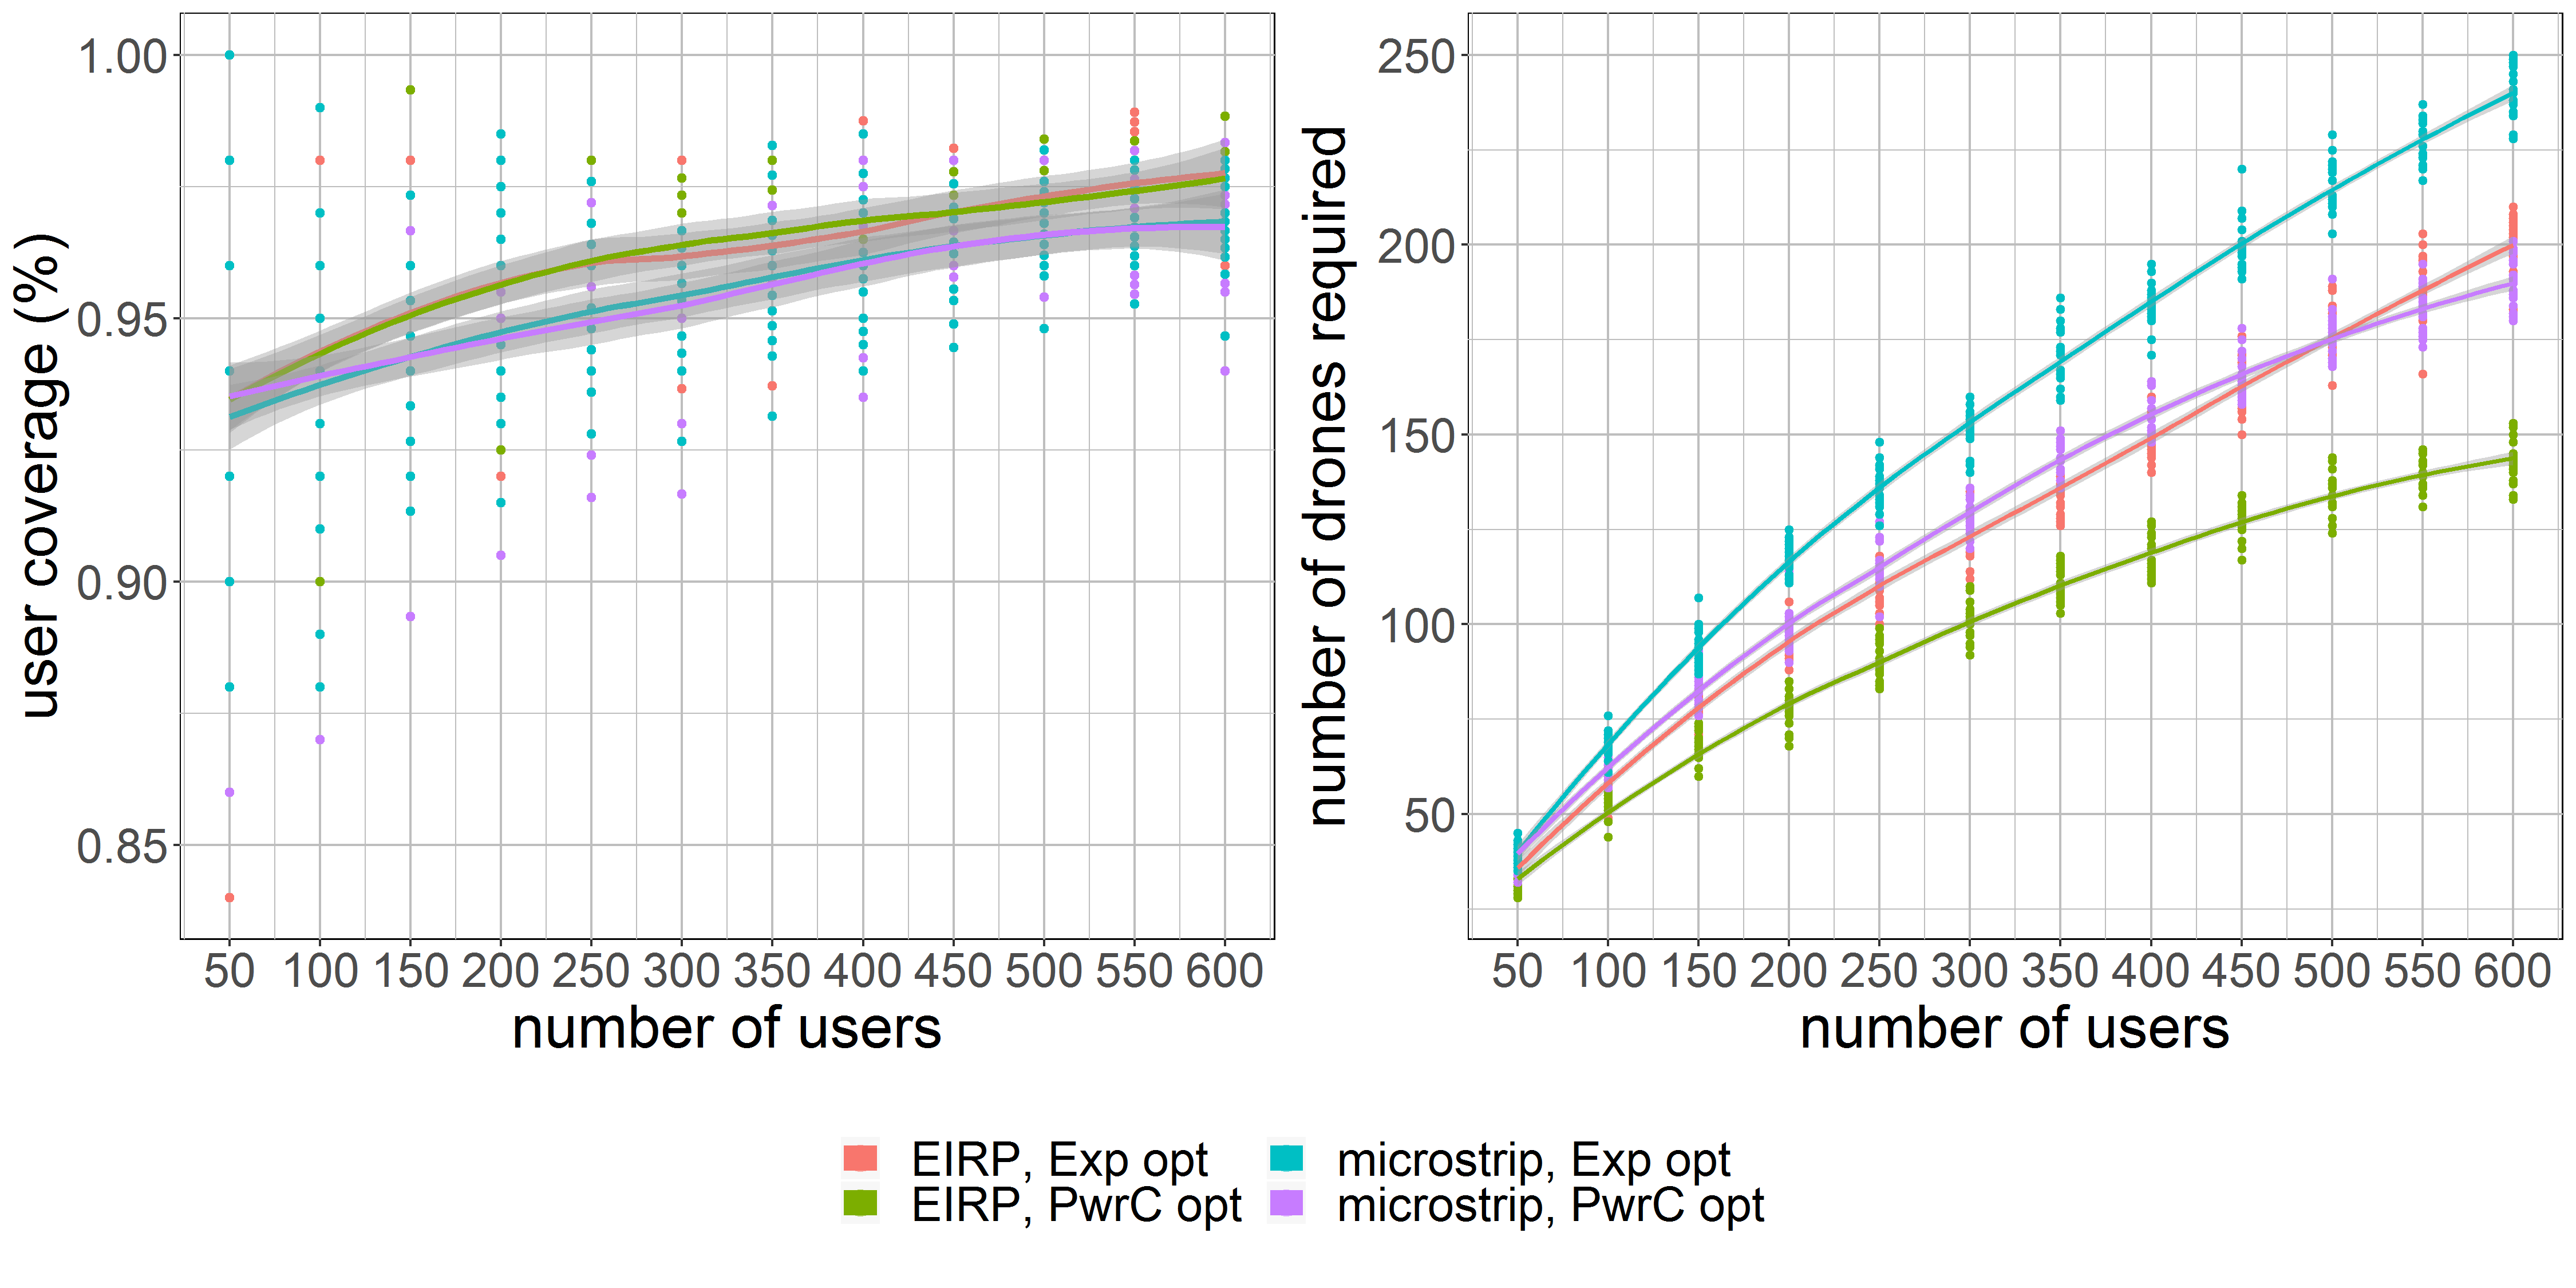
\includegraphics[width=\linewidth]{../results/s3/uvsnumdronesAndCov.png}
  \caption{Deze grafiek toont hoeveel drones vereist zijn op verschillende vlieghoogte's terwijl er getracht wordt een 100\% bereikt te hebben.}
  \label{fig:s3b_numdronesAndCov}
\end{figure}

Figuur \ref{fig:s3b_dlAndPC} Toont aan dat de elektromagnetische straling's en het energieverbruik toeneemt voor grotere populaties wat normaal is aangezien meer \gls{UABS}'s
beschikbaar zijn. Wanneer de populatie toeneemt van 50 naar 600 gebruikers zal 
de elektromagnetische straling toenemen tussen 80 en 130 $mV/m$ afhankelijk van de configuratie. 
Het energieverbruik bij 50 gebruikers is voor alle configuraties rond 20 $W$.
Eenmaal de populatie is toegenomen naar 600 gebruikers zal dit voor een
microstrip \gls{Exp Opt} netwerk 130 $W$ bedragen, 115 $W$ voor een microstrip \gls{PwrC Opt} netwerk,
102 $W$ voor een \gls{EIRP} \gls{Exp Opt} netwerk en 92 $W$ voor een  \gls{EIRP} \gls{PwrC Opt} netwerk.

Dat het beslissingsalgoritme werkt zoals bedoeld, werd reeds duidelijk in de voorgaande subsectie maar wordt
ook bevestigd hier. Wanneer beide optimalisatiestrategieën vergeleken worden 
blijkt dat een energiezuinig netwerk ongeveer 5 $W$ minder energie nodig heeft maar hierdoor de gebruikers wel aan 
bloodstelt aan 27 $mV/m$ and 30 $mV/m$ meer elektromagnetische straling ten opzichte van \gls{Exp Opt} netwerken.
Verder zal een \gls{isotropicradiator} ook meer elektromagnetische straling veroorzaken 
voor minder energie in vergelijking met een microstrip patch antenne.
Wanneer beide antennes vergeleken worden voor 224 gebruikers blijkt 
dat de \gls{isotropicradiator} de gemiddelde gebruiker tussen 
 25 $mV/m$ tot 27 $mV/m$ extra Elektromagnetisme zal blootstellen
 terwijl het gemiddeld 12 $W$ minder zal nodig hebben in vergelijking met de microstrip patch antenne.


\begin{figure}[h!]
  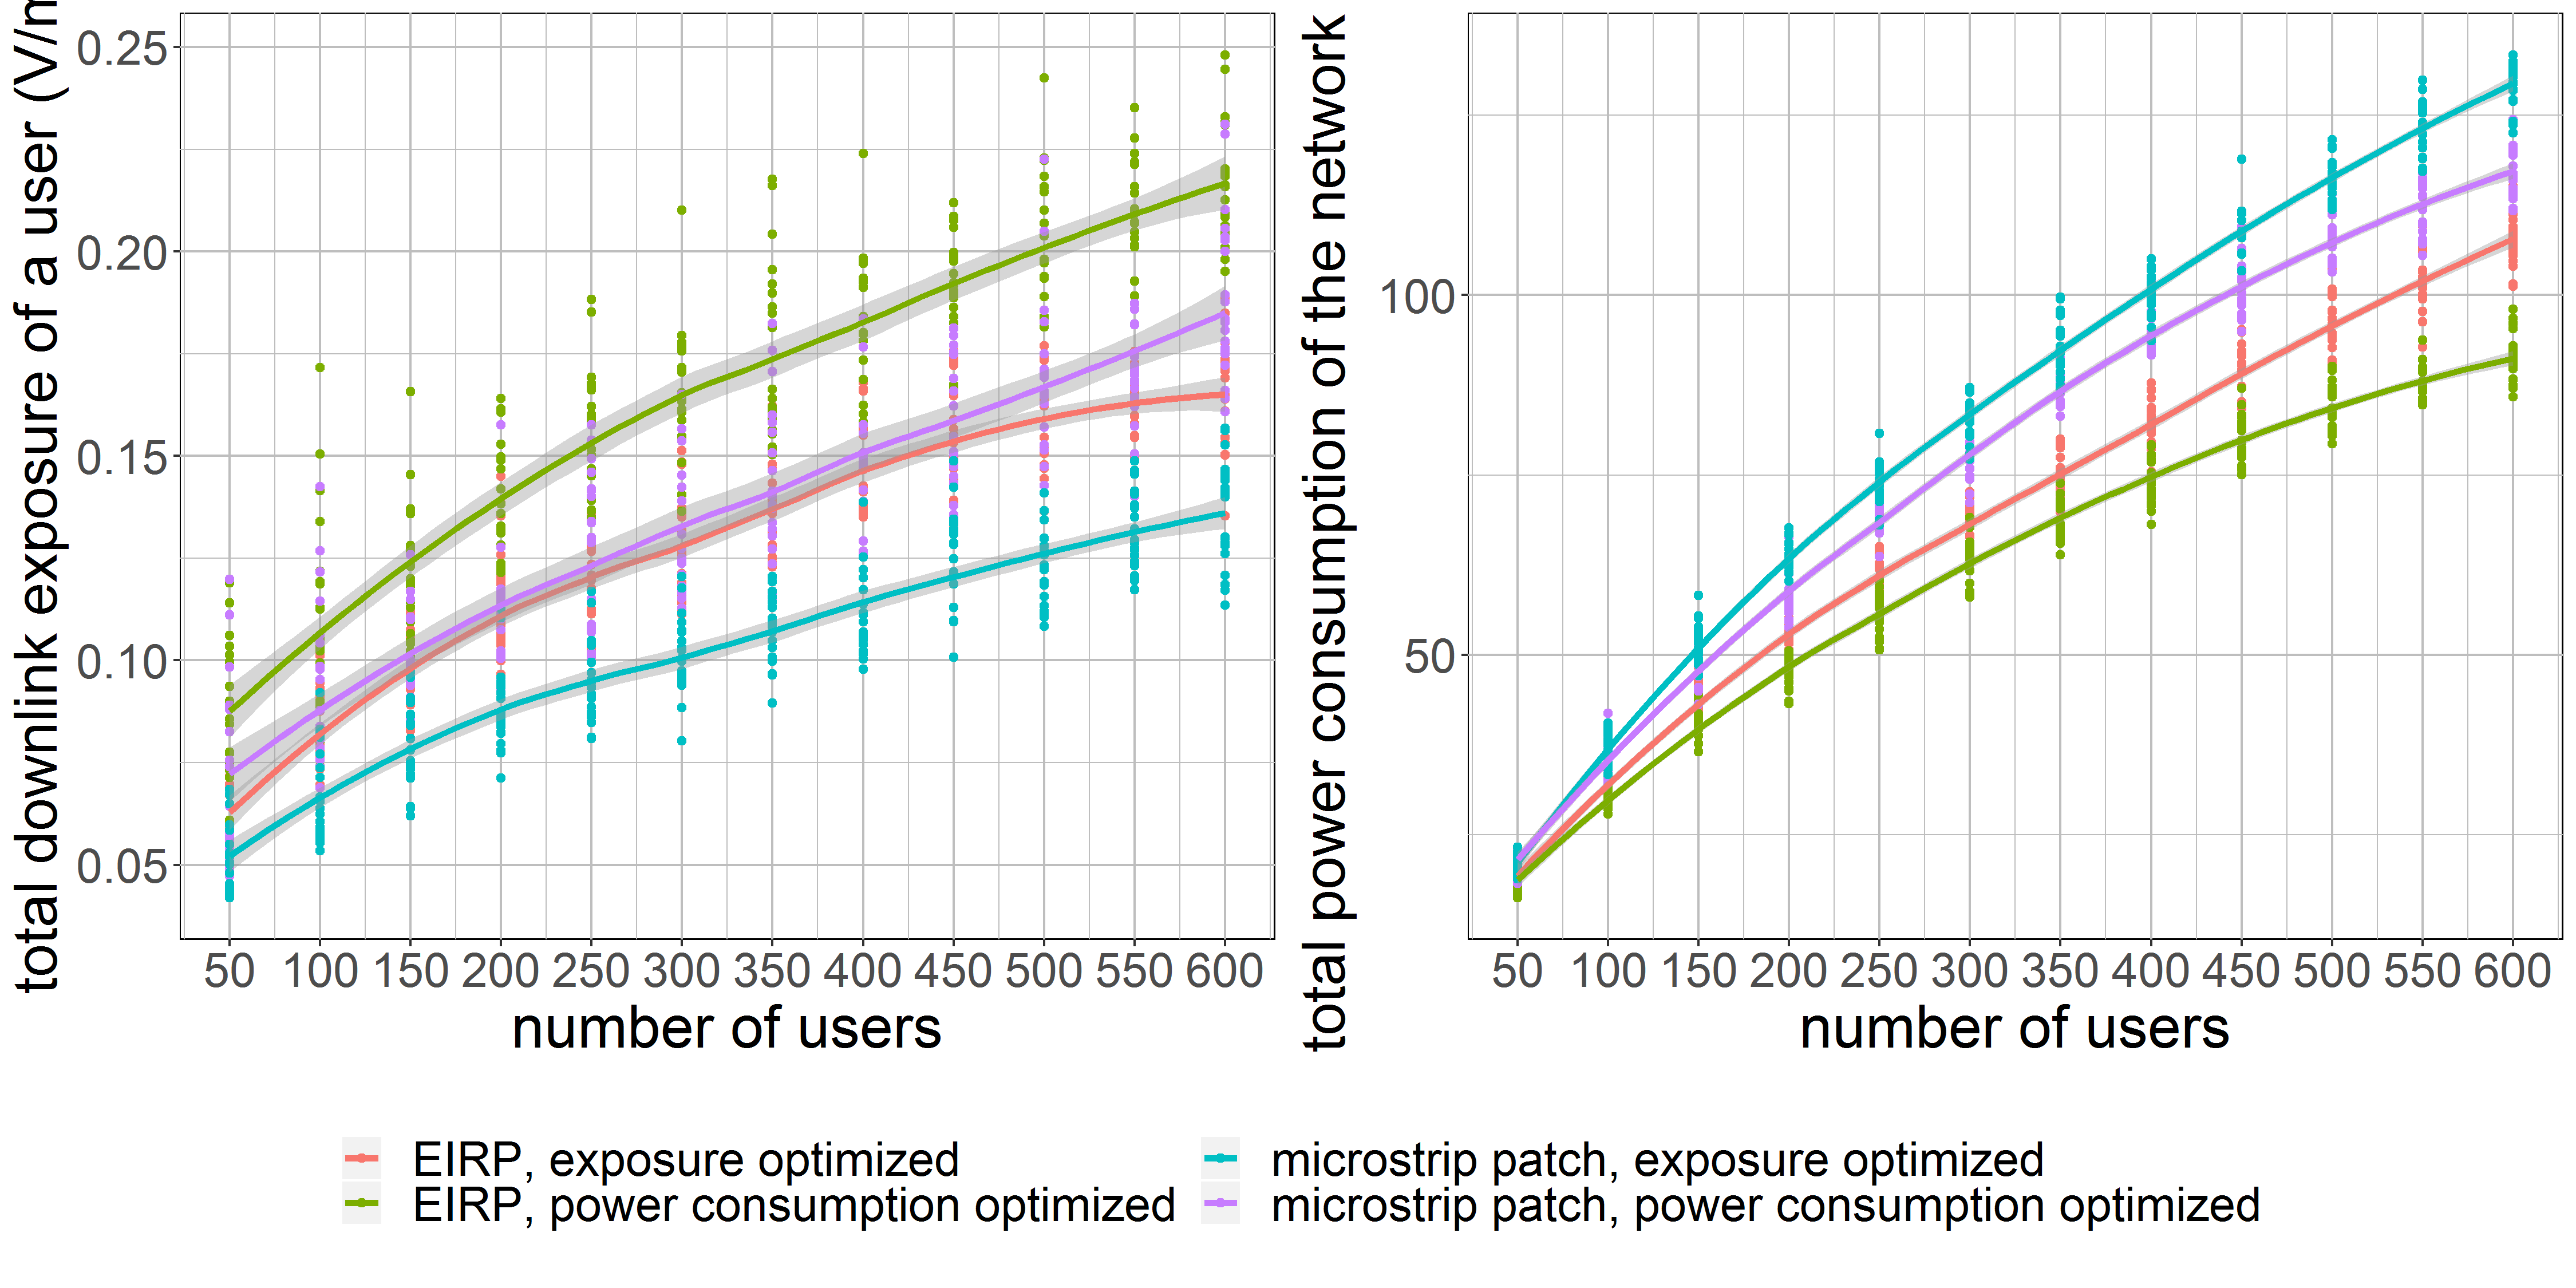
\includegraphics[width=\linewidth]{../results/s3/uvsdlAndPc.png}
  \caption{ De invloed van de populatiegrootte op de \acs{DL} elektromagnetische straling (a) en energieverbruik (b).
    }
  \label{fig:s3b_dlAndPC}
%\bigbreak
 % 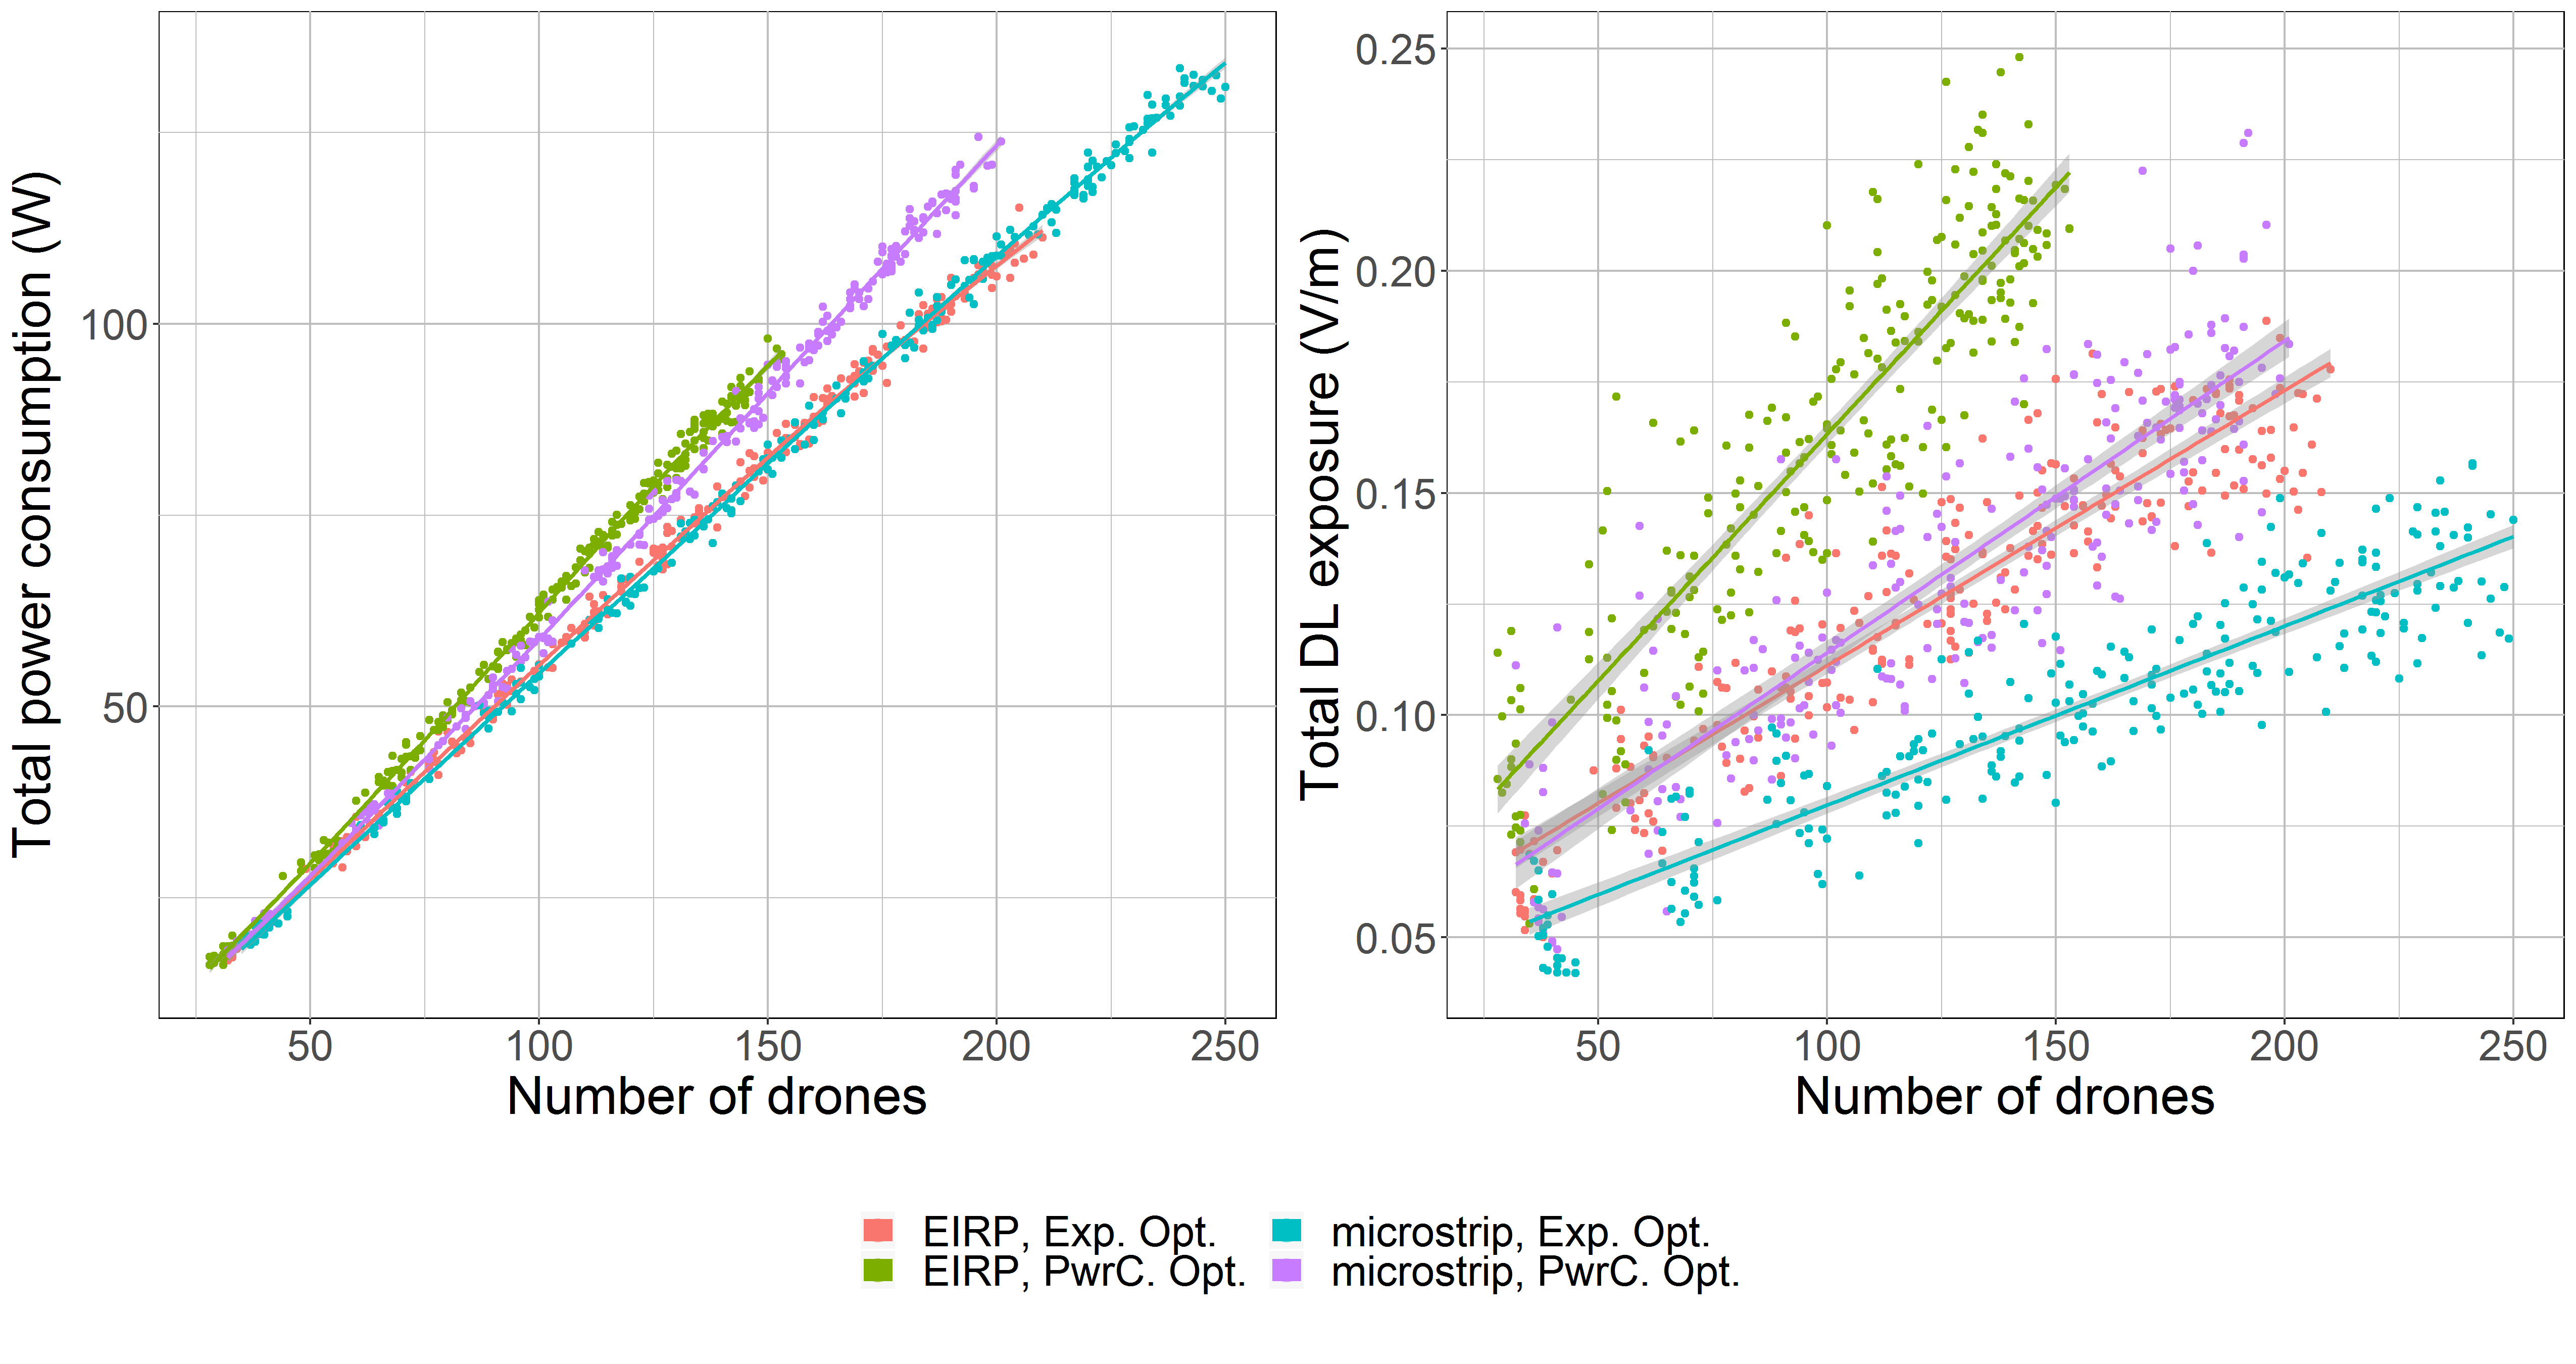
\includegraphics[width=\linewidth]{../results/s3/u_numdronesvsdlAndPc.png}
  %\caption{The influence of the number of UABSs on the downlink electromagnetic radiation (a) and power consumption (b).}
  %\label{fig:s3b_dlAndPC2}
\end{figure}


Figuur \ref{fig:s3b_fourSourcesMatrix} representeerd de  
\gls{SAR} van de gewogen gemiddelde gebruiker en toont aan hoe de 
\gls{SAR} van de gebruiker zijn eigen mobiele apparaat zo goed als constant is.
De vlieghoogte is namelijk altijd dezelfde wijn voor is ook de energie die nodig is om de afstand te overbruggen gelijk.
Voorbij de optimalisatiestrategie\"en zal de
 $SAR^{myUE}$ voor netwerken met  \gls{isotropicradiator}s vari\"eren rond $1.1\ \mu W/kg$  %between 1 $\mu W/kg$ and 1.2 $\mu W/kg$ 
 en rond 0.7 $\mu W/kg$ voor netwerken met een microstrip patch antenne.
De $SAR^{myUABS}$ Neemt nauwelijks toe in een \gls{Exp Opt} netwerk een bevindt zich rond 0.5 $\mu W/kg$ voor beide antennes.
Een energiezuinig netwerk start ook rond
 0.5 $\mu W/kg$ maar neemt toe wanneer meer mensen online komen.
Dit is normaal aangezien deze \gls{UABS}'s trachten om veel meer mensen te behandelen.
Hierdoor zal de $SAR^{myUABS}$ 
voor 600 users toenemen tot 1 $\mu W/kg$ voor een \gls{isotropicradiator} en tot wel 2 $\mu W/kg$ voor een microstrip patch antenne.
De \gls{SAR} waarde neemt het meeste toe bij $SAR^{otherUABS}$ dewelke heel laag start rond minder  dan  
0.1 $\mu W/kg$ voor 50 gebruikers in alle configuraties. 
Deze \gls{SAR} neemt echter snel toe. De grootste toename wordt waargenomen in een 
\gls{EIRP} \gls{PwrC Opt} netwerk 
waarbij 3 $\mu W/kg$ gemeten wordr voor 600 gebruikers. De $SAR^{otherUE}$ neemt het minste toe in een microstrip \gls{Exp Opt} met 
slecths 1 $\mu W/kg$ voor 600 gebruikers.
\begin{figure}[h!]
  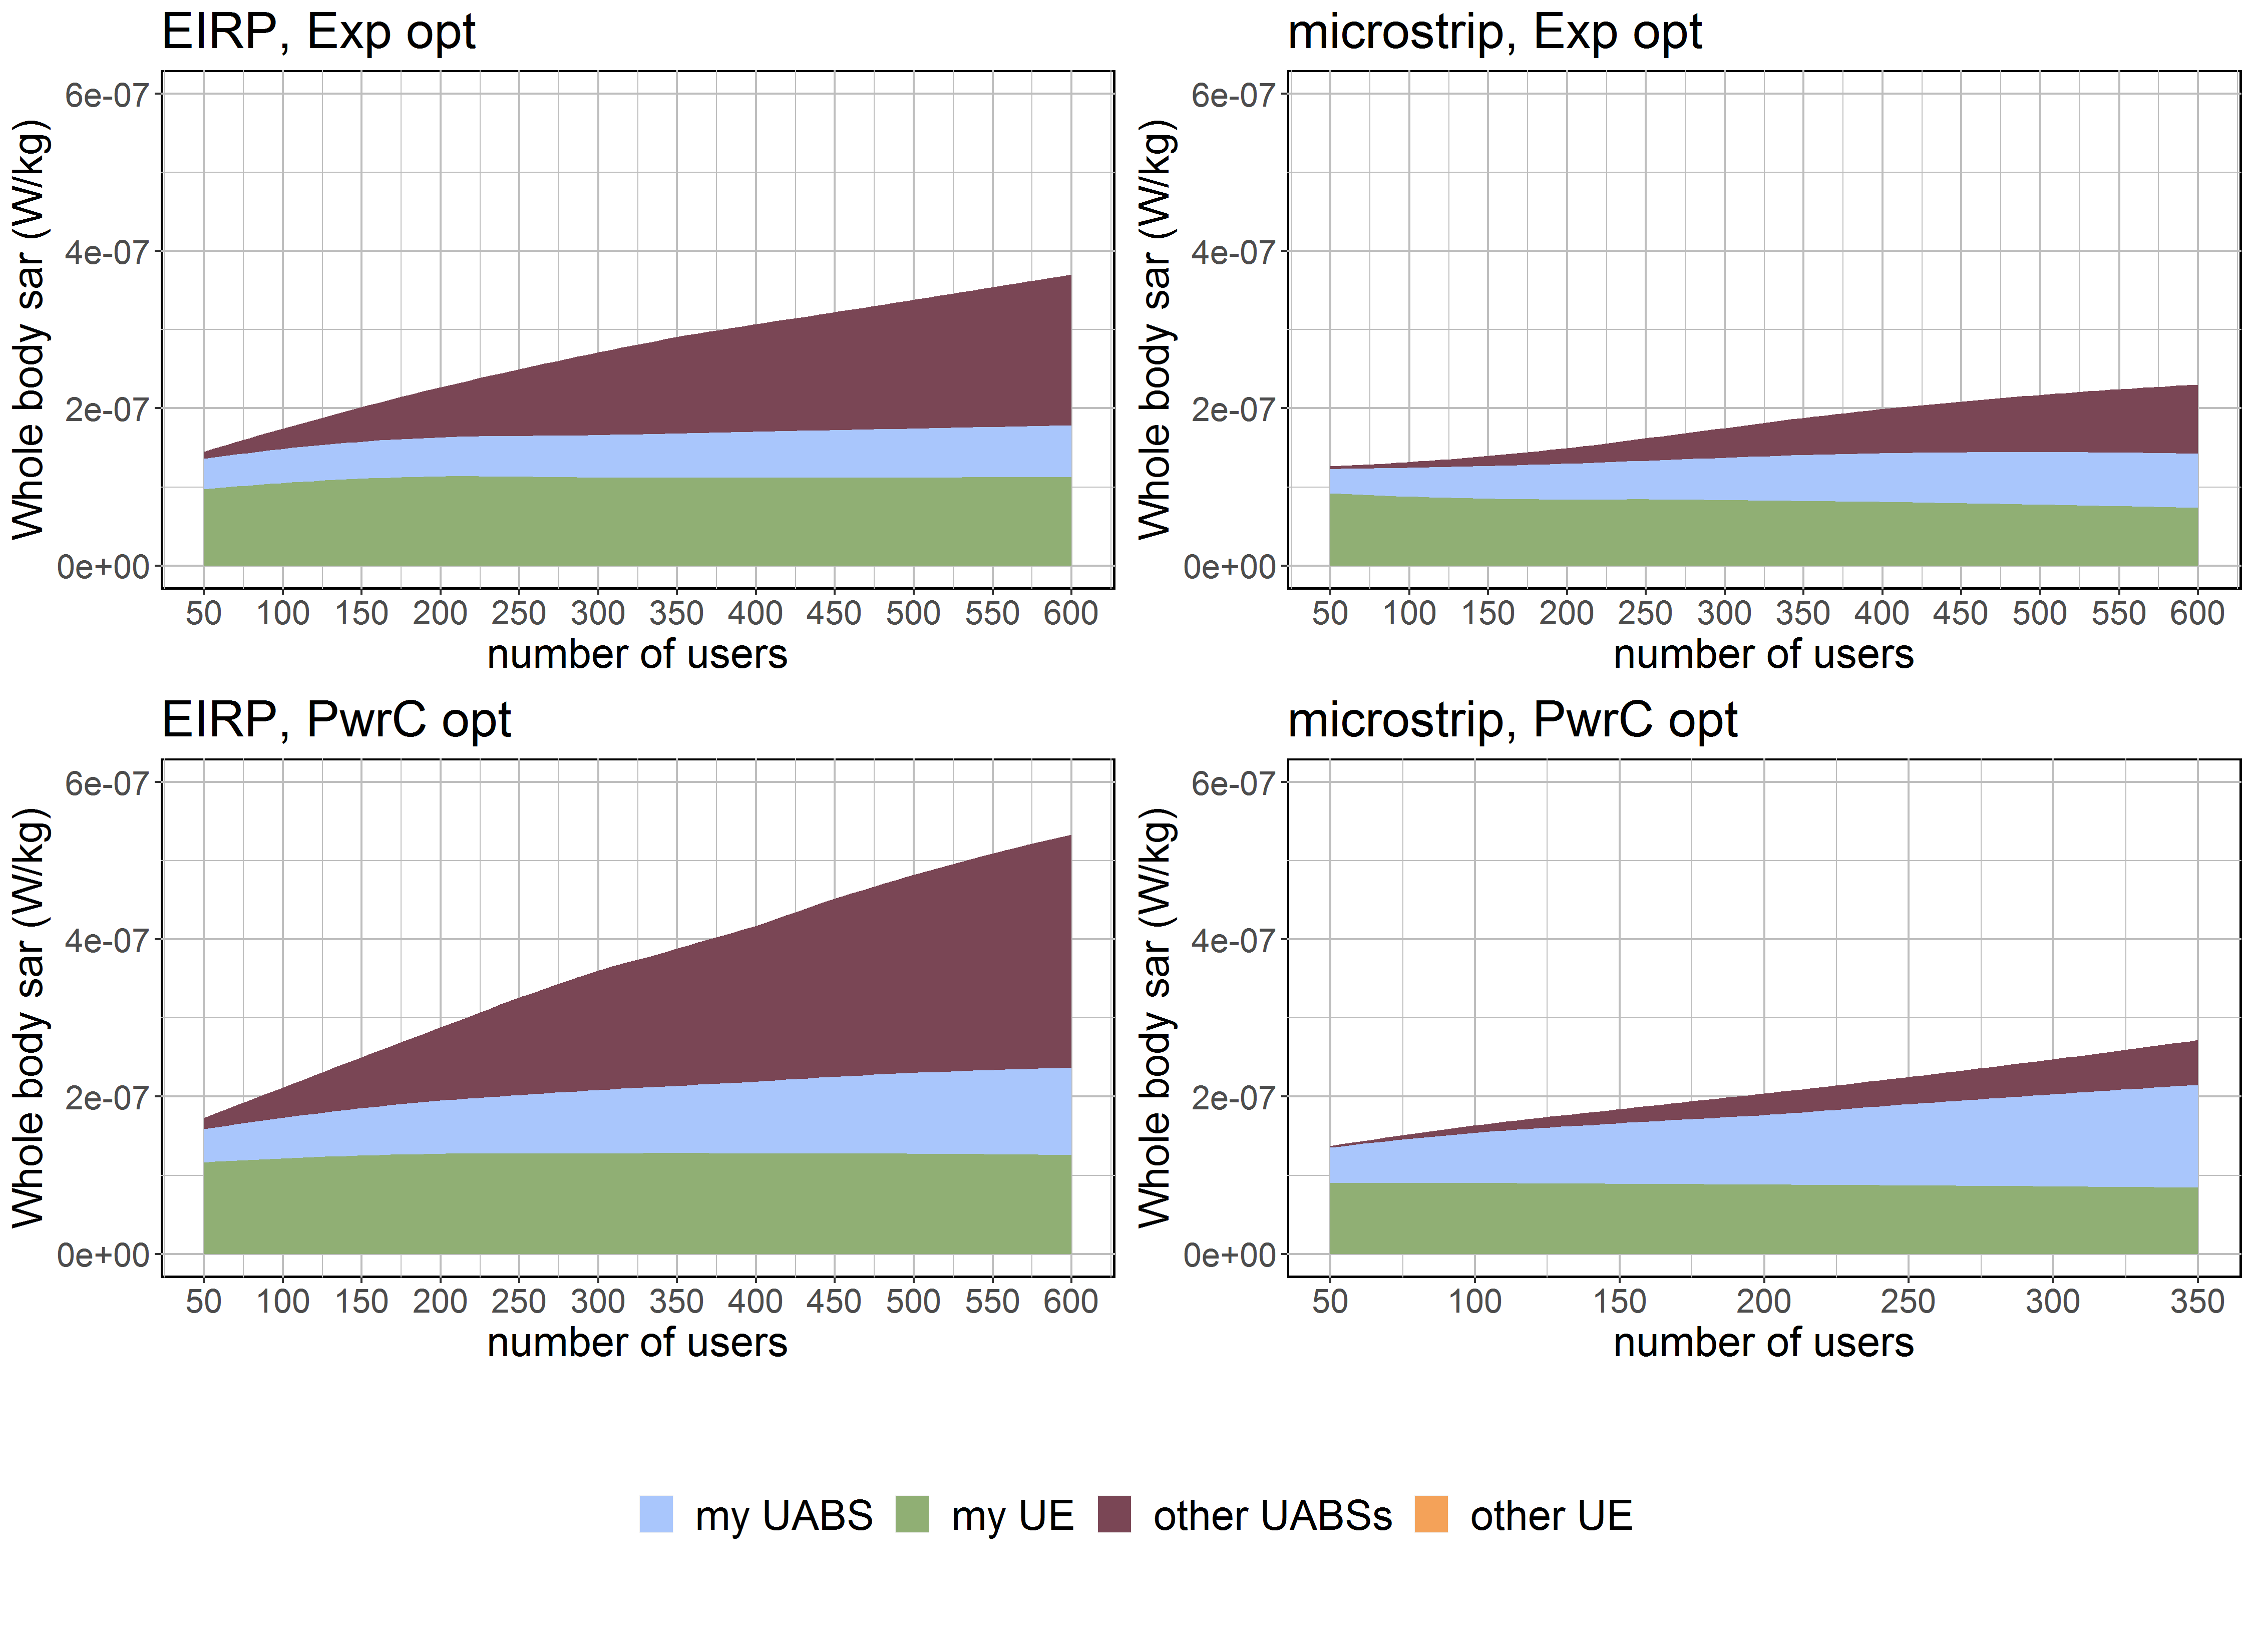
\includegraphics[width=\linewidth]{../results/s3/uFourSources.png}
  \caption{Elke grafiek komt overeen met een specifieke configuratie en toont aan hoe de \acs{SAR} 
  van verschillende bronnen be\"invloed wordt door een toenemende populatie. Een ongelimiteerd aantal \acs{UABS}s is beschikbaar.
}
  \label{fig:s3b_fourSourcesMatrix}
\end{figure}

\section{Conclusie}
%How can a UABS network be optimized to minimize global exposure or overall power consumption? 
Literature showed that a network can be optimized towards either the power consumption of the entire network 
or the electromagnetic exposure of the average user using a fitness function \cite{J1}.
However, the fitness function should be used with care considering that \gls{UABS}'s can be placed anywhere as opposed to 
the transmission towers from \cite{J1} who have a predetermined position. 
In an \gls{Exp Opt} network, this causes a lot of users to get a \gls{UABS} all by 
themselves because this is the best approach to minimize exposure.
A \gls{PwrC Opt} network on the other hand will try to limit the number of drones 
in order to save energy. 
So as a rule of thumb: an \gls{Exp Opt} network will result in a lot of low powered devices (increasing the overall power consumption)
while a \gls{PwrC Opt} network results in a few high powered devices (increasing the exposure of the average user).
If the goal is to remain in the air for a longer period of time, an \gls{Exp Opt} network is recommended because the power consumption of 
an individual \gls{UABS} is lower.
On the other hand, a \gls{PwrC Opt} network is cheaper because less drones are involved. 
Moreover, the results show that the electromagnetic radiation in a \gls{PwrC Opt} network (with high powered \gls{UABS}'s)
is far below the thresholds enforced by the Flemish government.

The user's main sources of exposure are the user's own device and the \gls{UABS} who is serving him, followed by all
other \gls{UABS}'s in the network. 
When the population increases, there is not only more radiation from \gls{UE} but also 
from more \gls{UABS}'s that are serving the other users.
The exposure from other people's \gls{UE} is so low that it can be neglected.
An \gls{Exp Opt} network will limit the total exposure mainly by trying to reduce the exposure from other \gls{UABS}'s.

%1)	How does the network behave differently after the introduction of a realistic antenna?
A directional microstrip patch antenna is introduced because it gives several advantages compared to omnidirectional antennae.
Directional antennae are able to focus their energy there where it is needed, namely towards the ground. Microstrip patch antennae 
further benefit from their thin and lightweight design. The performance 
of this directional microstrip patch antenna has been compared to a 
fictional \gls{isotropicradiator}.
This \gls{isotropicradiator} has higher exposure and coverage for less power, compared to realistic antennae like microstrip patch antennae
because of the absence of attenuation, and can hypothetically be compared with an antenna with a very big aperture angle.
This type of antenna can achieve the same coverage with less
resources like power and number of drones. 
A microstrip patch antenna with a more limited aperture angle of \ang{90} requires more resources but 
causes less sideways radiation. So the exposure from other \gls{UABS}'s will be way less.

\begin{figure}[h!]
  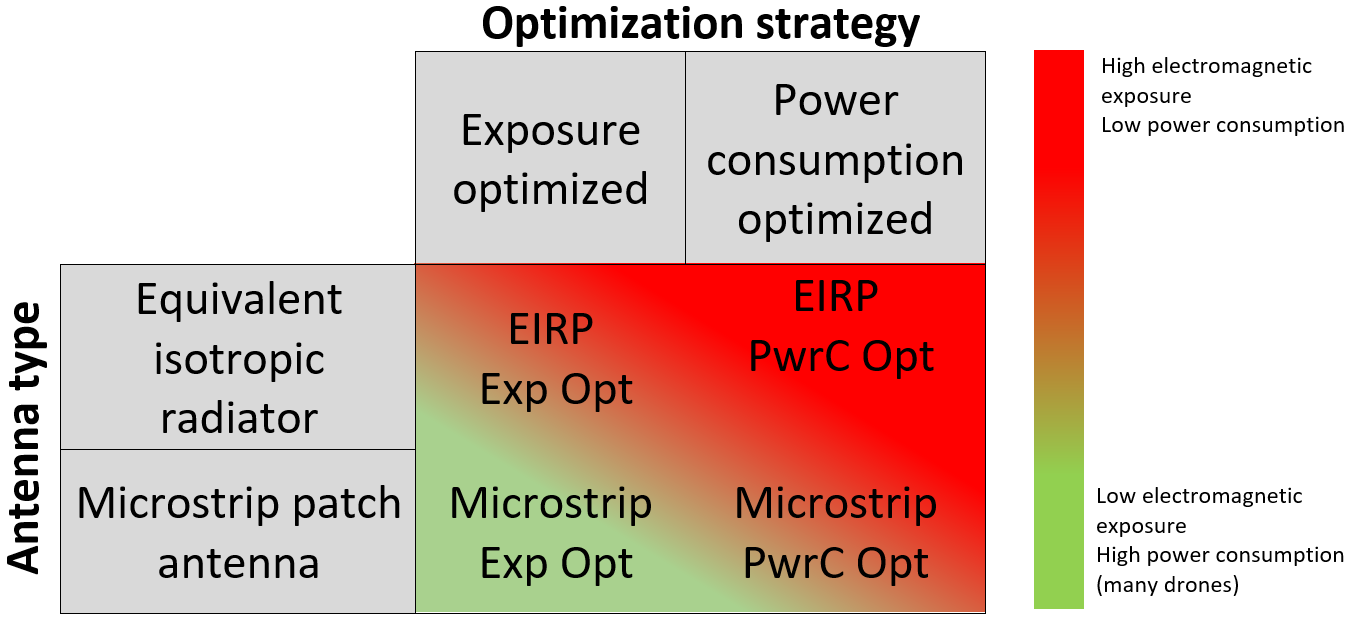
\includegraphics[width=\linewidth]{fourCasesMatrixSol.png}
  \caption{Matrix with the four possible configurations, colour-coded based on the results.}
  \label{fig:resultIllustration}
\end{figure}

Remarkable is that an \gls{EIRP} \gls{Exp Opt} network behaves very similar to a microstrip \gls{PwrC Opt} network as shown 
in figure \ref{fig:resultIllustration}.
This results in the best of both worlds. 
The microstrip patch antenna will generate less electromagnetic radiation by design and
 the power consumption optimization reduces the number of required drones and power. A microstrip patch antenna with an aperture 
 angle of \ang{90} is considered as a good solution but if budget is limited, an antenna with a larger aperture angle 
 would further reduce cost without interfering with the Flemish legislation regarding electromagnetic exposure.

The electromagnetic radiation of an \gls{Exp Opt} network increases with higher flying altitudes.
Around 80 metres, the exposure from the  user's device surpasses the exposure from the serving \gls{UABS}.
On the other hand, a \gls{PwrC Opt} network shows that the lowest exposure is measured around 70 to 80 metres.
Further, the results also show that the number of required drones decreases when the flying height becomes larger; a conclusion that was also made in \cite{J2}.
When also considering the results from \cite{U1} where a flying altitude from 
80 metres is suggested for an optimal access and backhaul connectivity, a flying height 
of 80 metres is also here proposed for the city centre of Ghent.

In short, a \gls{PwrC Opt} network is proposed with a fixed flying height of 80 metres. A microstrip patch 
antenna with a sufficiently large aperture angle is a good starting point. However, different antenna configurations should 
be investigated.

\section*{Dankwoord}
Special thanks to the WAVES research group at Ghent University for providing 
access to their capacity based deployment tool and therefore making this research possible.

\bibliographystyle{ieeetr}
\bibliography{referenties}


\end{document}
